\documentclass[twoside]{book}

% Packages required by doxygen
\usepackage{fixltx2e}
\usepackage{calc}
\usepackage{doxygen}
\usepackage[export]{adjustbox} % also loads graphicx
\usepackage{graphicx}
\usepackage[utf8]{inputenc}
\usepackage{makeidx}
\usepackage{multicol}
\usepackage{multirow}
\PassOptionsToPackage{warn}{textcomp}
\usepackage{textcomp}
\usepackage[nointegrals]{wasysym}
\usepackage[table]{xcolor}

% Font selection
\usepackage[T1]{fontenc}
\usepackage[scaled=.90]{helvet}
\usepackage{courier}
\usepackage{amssymb}
\usepackage{sectsty}
\renewcommand{\familydefault}{\sfdefault}
\allsectionsfont{%
  \fontseries{bc}\selectfont%
  \color{darkgray}%
}
\renewcommand{\DoxyLabelFont}{%
  \fontseries{bc}\selectfont%
  \color{darkgray}%
}
\newcommand{\+}{\discretionary{\mbox{\scriptsize$\hookleftarrow$}}{}{}}

% Page & text layout
\usepackage{geometry}
\geometry{%
  a4paper,%
  top=2.5cm,%
  bottom=2.5cm,%
  left=2.5cm,%
  right=2.5cm%
}
\tolerance=750
\hfuzz=15pt
\hbadness=750
\setlength{\emergencystretch}{15pt}
\setlength{\parindent}{0cm}
\setlength{\parskip}{0.2cm}
\makeatletter
\renewcommand{\paragraph}{%
  \@startsection{paragraph}{4}{0ex}{-1.0ex}{1.0ex}{%
    \normalfont\normalsize\bfseries\SS@parafont%
  }%
}
\renewcommand{\subparagraph}{%
  \@startsection{subparagraph}{5}{0ex}{-1.0ex}{1.0ex}{%
    \normalfont\normalsize\bfseries\SS@subparafont%
  }%
}
\makeatother

% Headers & footers
\usepackage{fancyhdr}
\pagestyle{fancyplain}
\fancyhead[LE]{\fancyplain{}{\bfseries\thepage}}
\fancyhead[CE]{\fancyplain{}{}}
\fancyhead[RE]{\fancyplain{}{\bfseries\leftmark}}
\fancyhead[LO]{\fancyplain{}{\bfseries\rightmark}}
\fancyhead[CO]{\fancyplain{}{}}
\fancyhead[RO]{\fancyplain{}{\bfseries\thepage}}
\fancyfoot[LE]{\fancyplain{}{}}
\fancyfoot[CE]{\fancyplain{}{}}
\fancyfoot[RE]{\fancyplain{}{\bfseries\scriptsize Generated on Mon Jun 20 2016 19\+:38\+:08 for 3\+D\+Placement by Doxygen }}
\fancyfoot[LO]{\fancyplain{}{\bfseries\scriptsize Generated on Mon Jun 20 2016 19\+:38\+:08 for 3\+D\+Placement by Doxygen }}
\fancyfoot[CO]{\fancyplain{}{}}
\fancyfoot[RO]{\fancyplain{}{}}
\renewcommand{\footrulewidth}{0.4pt}
\renewcommand{\chaptermark}[1]{%
  \markboth{#1}{}%
}
\renewcommand{\sectionmark}[1]{%
  \markright{\thesection\ #1}%
}

% Indices & bibliography
\usepackage{natbib}
\usepackage[titles]{tocloft}
\setcounter{tocdepth}{3}
\setcounter{secnumdepth}{5}
\makeindex

% Hyperlinks (required, but should be loaded last)
\usepackage{ifpdf}
\ifpdf
  \usepackage[pdftex,pagebackref=true]{hyperref}
\else
  \usepackage[ps2pdf,pagebackref=true]{hyperref}
\fi
\hypersetup{%
  colorlinks=true,%
  linkcolor=blue,%
  citecolor=blue,%
  unicode%
}

% Custom commands
\newcommand{\clearemptydoublepage}{%
  \newpage{\pagestyle{empty}\cleardoublepage}%
}


%===== C O N T E N T S =====

\begin{document}

% Titlepage & ToC
\hypersetup{pageanchor=false,
             bookmarks=true,
             bookmarksnumbered=true,
             pdfencoding=unicode
            }
\pagenumbering{roman}
\begin{titlepage}
\vspace*{7cm}
\begin{center}%
{\Large 3\+D\+Placement }\\
\vspace*{1cm}
{\large Generated by Doxygen 1.8.9.1}\\
\vspace*{0.5cm}
{\small Mon Jun 20 2016 19:38:08}\\
\end{center}
\end{titlepage}
\clearemptydoublepage
\tableofcontents
\clearemptydoublepage
\pagenumbering{arabic}
\hypersetup{pageanchor=true}

%--- Begin generated contents ---
\chapter{Contribution Notice}
\label{md_README}
\hypertarget{md_README}{}

\begin{DoxyItemize}
\item Please use 4 spaces instead of tabs to indent. You can configure your editor to replace tabs with spaces.
\item Remember to update Makefile after modifying include hierarchy. You can refer to doxygen docs for current include hierarchy.
\item Run {\ttfamily doxygen Doxyfile} in this directory to generate doxygen docs. 
\end{DoxyItemize}
\chapter{Hierarchical Index}
\section{Class Hierarchy}
This inheritance list is sorted roughly, but not completely, alphabetically\+:\begin{DoxyCompactList}
\item \contentsline{section}{Base\+\_\+data}{\pageref{classBase__data}}{}
\begin{DoxyCompactList}
\item \contentsline{section}{T\+Tree\+\_\+data}{\pageref{classTTree__data}}{}
\end{DoxyCompactList}
\item \contentsline{section}{Block}{\pageref{structBlock}}{}
\item \contentsline{section}{Placement\+:\+:Block\+With\+Pos}{\pageref{structPlacement_1_1BlockWithPos}}{}
\item \contentsline{section}{Contour\+List}{\pageref{classContourList}}{}
\item \contentsline{section}{T\+Tree\+:\+:Node}{\pageref{classTTree_1_1Node}}{}
\item \contentsline{section}{Contour\+List\+:\+:Node}{\pageref{structContourList_1_1Node}}{}
\item \contentsline{section}{Placement}{\pageref{classPlacement}}{}
\item \contentsline{section}{Random}{\pageref{classRandom}}{}
\item \contentsline{section}{Rotatable\+Block}{\pageref{structRotatableBlock}}{}
\item \contentsline{section}{S\+A\+\_\+2}{\pageref{classSA__2}}{}
\item \contentsline{section}{T\+Tree\+:\+:subtree\+\_\+t}{\pageref{structTTree_1_1subtree__t}}{}
\item \contentsline{section}{T\+Tree}{\pageref{classTTree}}{}
\end{DoxyCompactList}

\chapter{Class Index}
\section{Class List}
Here are the classes, structs, unions and interfaces with brief descriptions\+:\begin{DoxyCompactList}
\item\contentsline{section}{\hyperlink{structBlock}{Block} \\*Defines a block out of the coordinates }{\pageref{structBlock}}{}
\item\contentsline{section}{\hyperlink{structPlacement_1_1BlockWithPos}{Placement\+::\+Block\+With\+Pos} }{\pageref{structPlacement_1_1BlockWithPos}}{}
\item\contentsline{section}{\hyperlink{classContourList}{Contour\+List} \\*Defines a vertical contour doubly-\/linked list }{\pageref{classContourList}}{}
\item\contentsline{section}{\hyperlink{structContourList_1_1Node}{Contour\+List\+::\+Node} \\*A node of a contour list }{\pageref{structContourList_1_1Node}}{}
\item\contentsline{section}{\hyperlink{classTTree_1_1Node}{T\+Tree\+::\+Node} \\*Internal class. A node of T Tree }{\pageref{classTTree_1_1Node}}{}
\item\contentsline{section}{\hyperlink{classPlacement}{Placement} \\*A compact placement of blocks }{\pageref{classPlacement}}{}
\item\contentsline{section}{\hyperlink{classRandom}{Random} \\*Please to this file instead of generate random numbers by yourself }{\pageref{classRandom}}{}
\item\contentsline{section}{\hyperlink{structRotatableBlock}{Rotatable\+Block} }{\pageref{structRotatableBlock}}{}
\item\contentsline{section}{\hyperlink{classSA}{S\+A} \\*Simulated Annealing }{\pageref{classSA}}{}
\item\contentsline{section}{\hyperlink{structTTree_1_1subtree__t}{T\+Tree\+::subtree\+\_\+t} }{\pageref{structTTree_1_1subtree__t}}{}
\item\contentsline{section}{\hyperlink{classTTree}{T\+Tree} }{\pageref{classTTree}}{}
\end{DoxyCompactList}

\chapter{File Index}
\section{File List}
Here is a list of all files with brief descriptions\+:\begin{DoxyCompactList}
\item\contentsline{section}{\hyperlink{Block_8h}{Block.\+h} }{\pageref{Block_8h}}{}
\item\contentsline{section}{\hyperlink{ContourList_8cpp}{Contour\+List.\+cpp} }{\pageref{ContourList_8cpp}}{}
\item\contentsline{section}{\hyperlink{ContourList_8h}{Contour\+List.\+h} }{\pageref{ContourList_8h}}{}
\item\contentsline{section}{\hyperlink{main_8cpp}{main.\+cpp} }{\pageref{main_8cpp}}{}
\item\contentsline{section}{\hyperlink{Placement_8cpp}{Placement.\+cpp} }{\pageref{Placement_8cpp}}{}
\item\contentsline{section}{\hyperlink{Placement_8h}{Placement.\+h} }{\pageref{Placement_8h}}{}
\item\contentsline{section}{\hyperlink{Random_8cpp}{Random.\+cpp} }{\pageref{Random_8cpp}}{}
\item\contentsline{section}{\hyperlink{Random_8h}{Random.\+h} }{\pageref{Random_8h}}{}
\item\contentsline{section}{\hyperlink{test_8cpp}{test.\+cpp} }{\pageref{test_8cpp}}{}
\item\contentsline{section}{\hyperlink{TTree_8cpp}{T\+Tree.\+cpp} }{\pageref{TTree_8cpp}}{}
\item\contentsline{section}{\hyperlink{TTree_8h}{T\+Tree.\+h} }{\pageref{TTree_8h}}{}
\end{DoxyCompactList}

\chapter{Class Documentation}
\hypertarget{classBase__data}{}\section{Base\+\_\+data Class Reference}
\label{classBase__data}\index{Base\+\_\+data@{Base\+\_\+data}}


Data interface used by S\+A2.  




{\ttfamily \#include $<$Basedata.\+h$>$}



Inheritance diagram for Base\+\_\+data\+:
\nopagebreak
\begin{figure}[H]
\begin{center}
\leavevmode
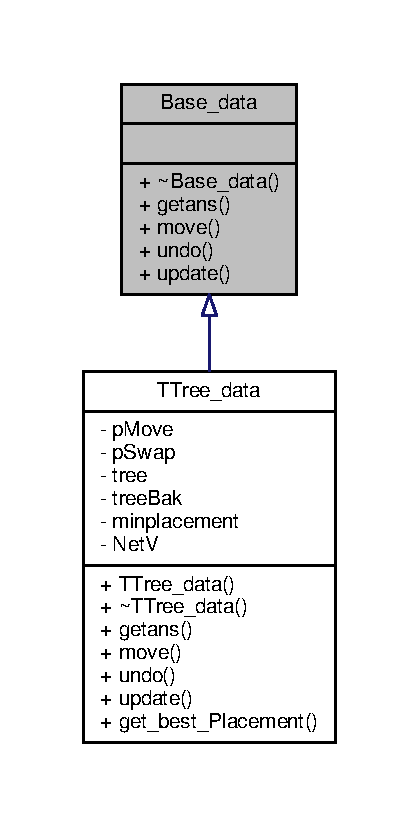
\includegraphics[width=201pt]{classBase__data__inherit__graph}
\end{center}
\end{figure}


Collaboration diagram for Base\+\_\+data\+:
\nopagebreak
\begin{figure}[H]
\begin{center}
\leavevmode
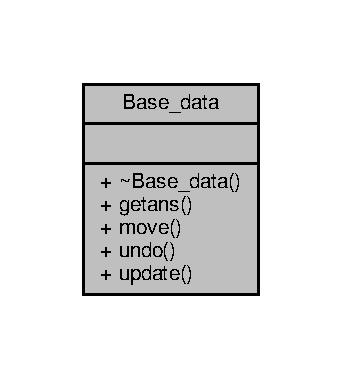
\includegraphics[width=164pt]{classBase__data__coll__graph}
\end{center}
\end{figure}
\subsection*{Public Member Functions}
\begin{DoxyCompactItemize}
\item 
virtual \hyperlink{classBase__data_aeea18956cb25b6bf02f651a923fb830a}{$\sim$\+Base\+\_\+data} ()
\item 
virtual double \hyperlink{classBase__data_a30c68b7fadf62354a5291e63c826a6b1}{getans} ()=0
\item 
virtual void \hyperlink{classBase__data_ae471e1151062f17bf299dc72dcfdd73a}{move} ()=0
\item 
virtual void \hyperlink{classBase__data_ab7486d1e6e1c199b637cb1473daf9a14}{undo} ()=0
\item 
virtual void \hyperlink{classBase__data_a8545b22fc79ece9d036731ecb3db7b5d}{update} ()=0
\end{DoxyCompactItemize}


\subsection{Detailed Description}
Data interface used by S\+A2. 

\subsection{Constructor \& Destructor Documentation}
\hypertarget{classBase__data_aeea18956cb25b6bf02f651a923fb830a}{}\index{Base\+\_\+data@{Base\+\_\+data}!````~Base\+\_\+data@{$\sim$\+Base\+\_\+data}}
\index{````~Base\+\_\+data@{$\sim$\+Base\+\_\+data}!Base\+\_\+data@{Base\+\_\+data}}
\subsubsection[{$\sim$\+Base\+\_\+data}]{\setlength{\rightskip}{0pt plus 5cm}virtual Base\+\_\+data\+::$\sim$\+Base\+\_\+data (
\begin{DoxyParamCaption}
{}
\end{DoxyParamCaption}
)\hspace{0.3cm}{\ttfamily [inline]}, {\ttfamily [virtual]}}\label{classBase__data_aeea18956cb25b6bf02f651a923fb830a}


\subsection{Member Function Documentation}
\hypertarget{classBase__data_a30c68b7fadf62354a5291e63c826a6b1}{}\index{Base\+\_\+data@{Base\+\_\+data}!getans@{getans}}
\index{getans@{getans}!Base\+\_\+data@{Base\+\_\+data}}
\subsubsection[{getans}]{\setlength{\rightskip}{0pt plus 5cm}virtual double Base\+\_\+data\+::getans (
\begin{DoxyParamCaption}
{}
\end{DoxyParamCaption}
)\hspace{0.3cm}{\ttfamily [pure virtual]}}\label{classBase__data_a30c68b7fadf62354a5291e63c826a6b1}


Implemented in \hyperlink{classTTree__data_a2524c0f18f01378fc80fd558e3b7cebb}{T\+Tree\+\_\+data}.

\hypertarget{classBase__data_ae471e1151062f17bf299dc72dcfdd73a}{}\index{Base\+\_\+data@{Base\+\_\+data}!move@{move}}
\index{move@{move}!Base\+\_\+data@{Base\+\_\+data}}
\subsubsection[{move}]{\setlength{\rightskip}{0pt plus 5cm}virtual void Base\+\_\+data\+::move (
\begin{DoxyParamCaption}
{}
\end{DoxyParamCaption}
)\hspace{0.3cm}{\ttfamily [pure virtual]}}\label{classBase__data_ae471e1151062f17bf299dc72dcfdd73a}


Implemented in \hyperlink{classTTree__data_a16a5d735999764d45d38d2327955696e}{T\+Tree\+\_\+data}.

\hypertarget{classBase__data_ab7486d1e6e1c199b637cb1473daf9a14}{}\index{Base\+\_\+data@{Base\+\_\+data}!undo@{undo}}
\index{undo@{undo}!Base\+\_\+data@{Base\+\_\+data}}
\subsubsection[{undo}]{\setlength{\rightskip}{0pt plus 5cm}virtual void Base\+\_\+data\+::undo (
\begin{DoxyParamCaption}
{}
\end{DoxyParamCaption}
)\hspace{0.3cm}{\ttfamily [pure virtual]}}\label{classBase__data_ab7486d1e6e1c199b637cb1473daf9a14}


Implemented in \hyperlink{classTTree__data_ac2f447392cb0cf81db44d4f85d4bfd8a}{T\+Tree\+\_\+data}.

\hypertarget{classBase__data_a8545b22fc79ece9d036731ecb3db7b5d}{}\index{Base\+\_\+data@{Base\+\_\+data}!update@{update}}
\index{update@{update}!Base\+\_\+data@{Base\+\_\+data}}
\subsubsection[{update}]{\setlength{\rightskip}{0pt plus 5cm}virtual void Base\+\_\+data\+::update (
\begin{DoxyParamCaption}
{}
\end{DoxyParamCaption}
)\hspace{0.3cm}{\ttfamily [pure virtual]}}\label{classBase__data_a8545b22fc79ece9d036731ecb3db7b5d}


Implemented in \hyperlink{classTTree__data_a828b99a40bab8933fd3c648ee4f10d85}{T\+Tree\+\_\+data}.



The documentation for this class was generated from the following file\+:\begin{DoxyCompactItemize}
\item 
\hyperlink{Basedata_8h}{Basedata.\+h}\end{DoxyCompactItemize}

\hypertarget{structBlock}{}\section{Block Struct Reference}
\label{structBlock}\index{Block@{Block}}


Defines a block out of the coordinates.  




{\ttfamily \#include $<$Block.\+h$>$}



Collaboration diagram for Block\+:
\nopagebreak
\begin{figure}[H]
\begin{center}
\leavevmode
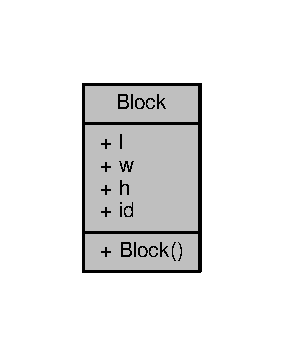
\includegraphics[width=136pt]{structBlock__coll__graph}
\end{center}
\end{figure}
\subsection*{Public Member Functions}
\begin{DoxyCompactItemize}
\item 
\hyperlink{structBlock_a832b4a589a691d3e10cfecc32398ddd0}{Block} (double \+\_\+l, double \+\_\+w, double \+\_\+h, int \+\_\+id=-\/1)
\begin{DoxyCompactList}\small\item\em optional. preserved to link to extra data. \end{DoxyCompactList}\end{DoxyCompactItemize}
\subsection*{Public Attributes}
\begin{DoxyCompactItemize}
\item 
double \hyperlink{structBlock_aad415a5d98d3645561306bf7d5bb22bb}{l}
\item 
double \hyperlink{structBlock_ae072df7850e56bf12d0234773e7eaa46}{w}
\item 
double \hyperlink{structBlock_a27826799e87ce49b8b1b72e7e2384583}{h}
\item 
int \hyperlink{structBlock_a86f38c868a8dab090101db6492078071}{id}
\begin{DoxyCompactList}\small\item\em corresponding to x, y, z axies. \end{DoxyCompactList}\end{DoxyCompactItemize}


\subsection{Detailed Description}
Defines a block out of the coordinates. 

This is determined by input and will not modified in the algorithm. 

\subsection{Constructor \& Destructor Documentation}
\hypertarget{structBlock_a832b4a589a691d3e10cfecc32398ddd0}{}\index{Block@{Block}!Block@{Block}}
\index{Block@{Block}!Block@{Block}}
\subsubsection[{Block}]{\setlength{\rightskip}{0pt plus 5cm}Block\+::\+Block (
\begin{DoxyParamCaption}
\item[{double}]{\+\_\+l, }
\item[{double}]{\+\_\+w, }
\item[{double}]{\+\_\+h, }
\item[{int}]{\+\_\+id = {\ttfamily -\/1}}
\end{DoxyParamCaption}
)\hspace{0.3cm}{\ttfamily [inline]}}\label{structBlock_a832b4a589a691d3e10cfecc32398ddd0}


optional. preserved to link to extra data. 



\subsection{Member Data Documentation}
\hypertarget{structBlock_a27826799e87ce49b8b1b72e7e2384583}{}\index{Block@{Block}!h@{h}}
\index{h@{h}!Block@{Block}}
\subsubsection[{h}]{\setlength{\rightskip}{0pt plus 5cm}double Block\+::h}\label{structBlock_a27826799e87ce49b8b1b72e7e2384583}
\hypertarget{structBlock_a86f38c868a8dab090101db6492078071}{}\index{Block@{Block}!id@{id}}
\index{id@{id}!Block@{Block}}
\subsubsection[{id}]{\setlength{\rightskip}{0pt plus 5cm}int Block\+::id}\label{structBlock_a86f38c868a8dab090101db6492078071}


corresponding to x, y, z axies. 

\hypertarget{structBlock_aad415a5d98d3645561306bf7d5bb22bb}{}\index{Block@{Block}!l@{l}}
\index{l@{l}!Block@{Block}}
\subsubsection[{l}]{\setlength{\rightskip}{0pt plus 5cm}double Block\+::l}\label{structBlock_aad415a5d98d3645561306bf7d5bb22bb}
\hypertarget{structBlock_ae072df7850e56bf12d0234773e7eaa46}{}\index{Block@{Block}!w@{w}}
\index{w@{w}!Block@{Block}}
\subsubsection[{w}]{\setlength{\rightskip}{0pt plus 5cm}double Block\+::w}\label{structBlock_ae072df7850e56bf12d0234773e7eaa46}


The documentation for this struct was generated from the following file\+:\begin{DoxyCompactItemize}
\item 
\hyperlink{Block_8h}{Block.\+h}\end{DoxyCompactItemize}

\hypertarget{structPlacement_1_1BlockWithPos}{}\section{Placement\+:\+:Block\+With\+Pos Struct Reference}
\label{structPlacement_1_1BlockWithPos}\index{Placement\+::\+Block\+With\+Pos@{Placement\+::\+Block\+With\+Pos}}


{\ttfamily \#include $<$Placement.\+h$>$}



Collaboration diagram for Placement\+:\+:Block\+With\+Pos\+:\nopagebreak
\begin{figure}[H]
\begin{center}
\leavevmode
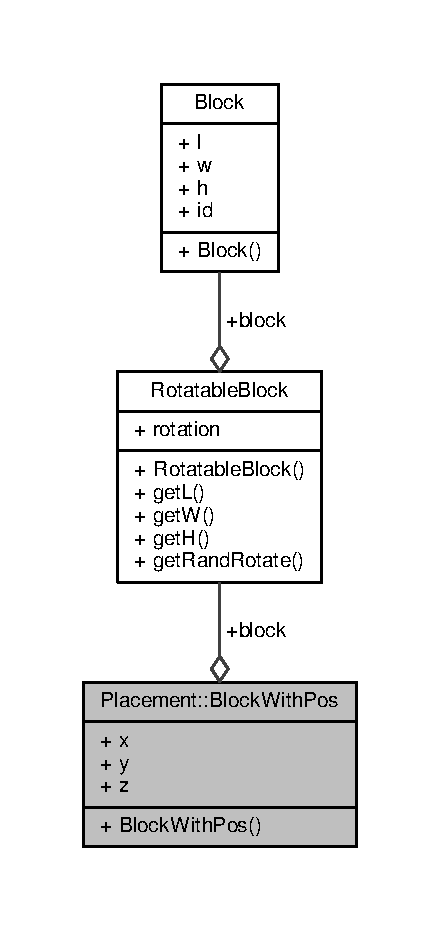
\includegraphics[width=211pt]{structPlacement_1_1BlockWithPos__coll__graph}
\end{center}
\end{figure}
\subsection*{Public Member Functions}
\begin{DoxyCompactItemize}
\item 
\hyperlink{structPlacement_1_1BlockWithPos_afb4a4cc160f62d32983def80899d01ac}{Block\+With\+Pos} (const \hyperlink{structRotatableBlock}{Rotatable\+Block} \&\+\_\+block, double \+\_\+x, double \+\_\+y, double \+\_\+z)
\end{DoxyCompactItemize}
\subsection*{Public Attributes}
\begin{DoxyCompactItemize}
\item 
\hyperlink{structRotatableBlock}{Rotatable\+Block} \hyperlink{structPlacement_1_1BlockWithPos_a152d1b38cdbe97057acf2ecb586c9d4e}{block}
\item 
double \hyperlink{structPlacement_1_1BlockWithPos_a9bead5b77b52b62474f1533c51bc9ff1}{x}
\item 
double \hyperlink{structPlacement_1_1BlockWithPos_acf2edddd35e7a041a454756157f063b1}{y}
\item 
double \hyperlink{structPlacement_1_1BlockWithPos_a31b55f7655dfeebab414dc668eb4d1c2}{z}
\end{DoxyCompactItemize}


\subsection{Constructor \& Destructor Documentation}
\hypertarget{structPlacement_1_1BlockWithPos_afb4a4cc160f62d32983def80899d01ac}{}\index{Placement\+::\+Block\+With\+Pos@{Placement\+::\+Block\+With\+Pos}!Block\+With\+Pos@{Block\+With\+Pos}}
\index{Block\+With\+Pos@{Block\+With\+Pos}!Placement\+::\+Block\+With\+Pos@{Placement\+::\+Block\+With\+Pos}}
\subsubsection[{Block\+With\+Pos}]{\setlength{\rightskip}{0pt plus 5cm}Placement\+::\+Block\+With\+Pos\+::\+Block\+With\+Pos (
\begin{DoxyParamCaption}
\item[{const {\bf Rotatable\+Block} \&}]{\+\_\+block, }
\item[{double}]{\+\_\+x, }
\item[{double}]{\+\_\+y, }
\item[{double}]{\+\_\+z}
\end{DoxyParamCaption}
)\hspace{0.3cm}{\ttfamily [inline]}}\label{structPlacement_1_1BlockWithPos_afb4a4cc160f62d32983def80899d01ac}


\subsection{Member Data Documentation}
\hypertarget{structPlacement_1_1BlockWithPos_a152d1b38cdbe97057acf2ecb586c9d4e}{}\index{Placement\+::\+Block\+With\+Pos@{Placement\+::\+Block\+With\+Pos}!block@{block}}
\index{block@{block}!Placement\+::\+Block\+With\+Pos@{Placement\+::\+Block\+With\+Pos}}
\subsubsection[{block}]{\setlength{\rightskip}{0pt plus 5cm}{\bf Rotatable\+Block} Placement\+::\+Block\+With\+Pos\+::block}\label{structPlacement_1_1BlockWithPos_a152d1b38cdbe97057acf2ecb586c9d4e}
\hypertarget{structPlacement_1_1BlockWithPos_a9bead5b77b52b62474f1533c51bc9ff1}{}\index{Placement\+::\+Block\+With\+Pos@{Placement\+::\+Block\+With\+Pos}!x@{x}}
\index{x@{x}!Placement\+::\+Block\+With\+Pos@{Placement\+::\+Block\+With\+Pos}}
\subsubsection[{x}]{\setlength{\rightskip}{0pt plus 5cm}double Placement\+::\+Block\+With\+Pos\+::x}\label{structPlacement_1_1BlockWithPos_a9bead5b77b52b62474f1533c51bc9ff1}
\hypertarget{structPlacement_1_1BlockWithPos_acf2edddd35e7a041a454756157f063b1}{}\index{Placement\+::\+Block\+With\+Pos@{Placement\+::\+Block\+With\+Pos}!y@{y}}
\index{y@{y}!Placement\+::\+Block\+With\+Pos@{Placement\+::\+Block\+With\+Pos}}
\subsubsection[{y}]{\setlength{\rightskip}{0pt plus 5cm}double Placement\+::\+Block\+With\+Pos\+::y}\label{structPlacement_1_1BlockWithPos_acf2edddd35e7a041a454756157f063b1}
\hypertarget{structPlacement_1_1BlockWithPos_a31b55f7655dfeebab414dc668eb4d1c2}{}\index{Placement\+::\+Block\+With\+Pos@{Placement\+::\+Block\+With\+Pos}!z@{z}}
\index{z@{z}!Placement\+::\+Block\+With\+Pos@{Placement\+::\+Block\+With\+Pos}}
\subsubsection[{z}]{\setlength{\rightskip}{0pt plus 5cm}double Placement\+::\+Block\+With\+Pos\+::z}\label{structPlacement_1_1BlockWithPos_a31b55f7655dfeebab414dc668eb4d1c2}


The documentation for this struct was generated from the following file\+:\begin{DoxyCompactItemize}
\item 
\hyperlink{Placement_8h}{Placement.\+h}\end{DoxyCompactItemize}

\hypertarget{classContourList}{}\section{Contour\+List Class Reference}
\label{classContourList}\index{Contour\+List@{Contour\+List}}


Defines a vertical contour doubly-\/linked list.  




{\ttfamily \#include $<$Contour\+List.\+h$>$}



Collaboration diagram for Contour\+List\+:\nopagebreak
\begin{figure}[H]
\begin{center}
\leavevmode
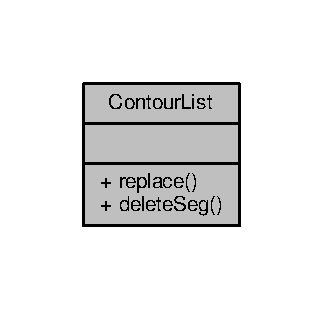
\includegraphics[width=155pt]{classContourList__coll__graph}
\end{center}
\end{figure}
\subsection*{Classes}
\begin{DoxyCompactItemize}
\item 
struct \hyperlink{structContourList_1_1Node}{Node}
\begin{DoxyCompactList}\small\item\em A node of a contour list. \end{DoxyCompactList}\end{DoxyCompactItemize}
\subsection*{Static Public Member Functions}
\begin{DoxyCompactItemize}
\item 
static \hyperlink{structContourList_1_1Node}{Node} $\ast$ \hyperlink{classContourList_a62250bf789d26d3392001287047e8d13}{replace} (\hyperlink{structContourList_1_1Node}{Node} $\ast$p, double \+\_\+z1, double \+\_\+z2)
\begin{DoxyCompactList}\small\item\em Replace a segment of nodes with a node. \end{DoxyCompactList}\item 
static void \hyperlink{classContourList_add57efb2cdaba0626be3138c91f5d43a}{delete\+Seg} (\hyperlink{structContourList_1_1Node}{Node} $\ast$l, \hyperlink{structContourList_1_1Node}{Node} $\ast$p, \hyperlink{structContourList_1_1Node}{Node} $\ast$r)
\begin{DoxyCompactList}\small\item\em Delete a segement of nodes starting from p, next to l, right to r i.\+e. range (l, r) p must in the range. \end{DoxyCompactList}\end{DoxyCompactItemize}


\subsection{Detailed Description}
Defines a vertical contour doubly-\/linked list. 

\subsection{Member Function Documentation}
\hypertarget{classContourList_add57efb2cdaba0626be3138c91f5d43a}{}\index{Contour\+List@{Contour\+List}!delete\+Seg@{delete\+Seg}}
\index{delete\+Seg@{delete\+Seg}!Contour\+List@{Contour\+List}}
\subsubsection[{delete\+Seg}]{\setlength{\rightskip}{0pt plus 5cm}void Contour\+List\+::delete\+Seg (
\begin{DoxyParamCaption}
\item[{{\bf Contour\+List\+::\+Node} $\ast$}]{l, }
\item[{{\bf Contour\+List\+::\+Node} $\ast$}]{p, }
\item[{{\bf Contour\+List\+::\+Node} $\ast$}]{r}
\end{DoxyParamCaption}
)\hspace{0.3cm}{\ttfamily [static]}}\label{classContourList_add57efb2cdaba0626be3138c91f5d43a}


Delete a segement of nodes starting from p, next to l, right to r i.\+e. range (l, r) p must in the range. 

\hypertarget{classContourList_a62250bf789d26d3392001287047e8d13}{}\index{Contour\+List@{Contour\+List}!replace@{replace}}
\index{replace@{replace}!Contour\+List@{Contour\+List}}
\subsubsection[{replace}]{\setlength{\rightskip}{0pt plus 5cm}{\bf Contour\+List\+::\+Node} $\ast$ Contour\+List\+::replace (
\begin{DoxyParamCaption}
\item[{{\bf Contour\+List\+::\+Node} $\ast$}]{p, }
\item[{double}]{\+\_\+z1, }
\item[{double}]{\+\_\+z2}
\end{DoxyParamCaption}
)\hspace{0.3cm}{\ttfamily [static]}}\label{classContourList_a62250bf789d26d3392001287047e8d13}


Replace a segment of nodes with a node. 

\begin{DoxyReturn}{Returns}
\+: the new node 
\end{DoxyReturn}


The documentation for this class was generated from the following files\+:\begin{DoxyCompactItemize}
\item 
\hyperlink{ContourList_8h}{Contour\+List.\+h}\item 
\hyperlink{ContourList_8cpp}{Contour\+List.\+cpp}\end{DoxyCompactItemize}

\hypertarget{classTTree_1_1Node}{}\section{T\+Tree\+:\+:Node Class Reference}
\label{classTTree_1_1Node}\index{T\+Tree\+::\+Node@{T\+Tree\+::\+Node}}


Internal class. A node of T Tree.  




Collaboration diagram for T\+Tree\+:\+:Node\+:
\nopagebreak
\begin{figure}[H]
\begin{center}
\leavevmode
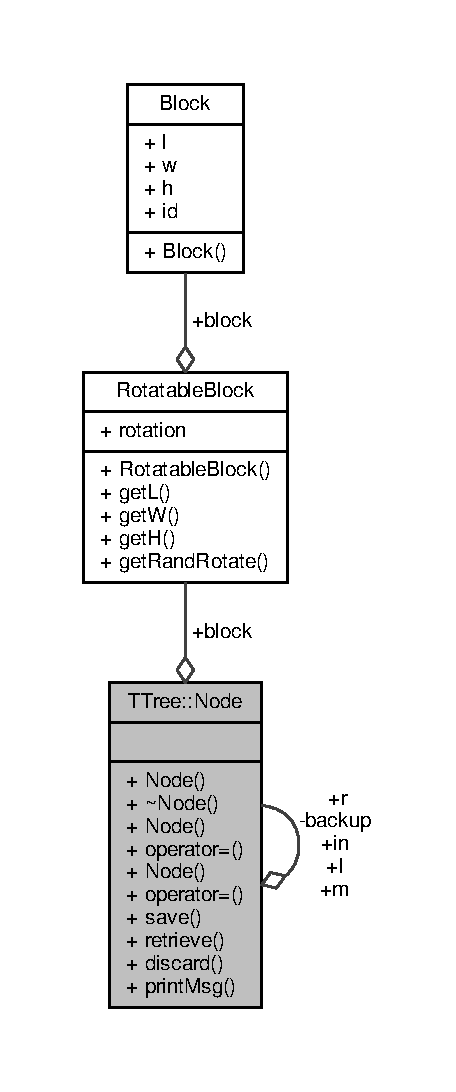
\includegraphics[width=219pt]{classTTree_1_1Node__coll__graph}
\end{center}
\end{figure}
\subsection*{Public Member Functions}
\begin{DoxyCompactItemize}
\item 
\hyperlink{classTTree_1_1Node_a73f229145664a7b5ce0c41746ba4e881}{Node} (const \hyperlink{structRotatableBlock}{Rotatable\+Block} \&\+\_\+block, \hyperlink{classTTree_1_1Node}{Node} $\ast$\+\_\+l=N\+U\+L\+L, \hyperlink{classTTree_1_1Node}{Node} $\ast$\+\_\+m=N\+U\+L\+L, \hyperlink{classTTree_1_1Node}{Node} $\ast$\+\_\+r=N\+U\+L\+L, \hyperlink{classTTree_1_1Node}{Node} $\ast$$\ast$\+\_\+in=N\+U\+L\+L)
\begin{DoxyCompactList}\small\item\em points to pointer point in the node. e.\+g. = \&(parent-\/$>$l) or \&root. \end{DoxyCompactList}\item 
\hyperlink{classTTree_1_1Node_a464e50288304ef7e9257a182125a474a}{$\sim$\+Node} ()
\item 
\hyperlink{classTTree_1_1Node_a6b9ce78ca08f3648379cf135d6796092}{Node} (const \hyperlink{classTTree_1_1Node}{Node} \&)=delete
\item 
\hyperlink{classTTree_1_1Node}{Node} \& \hyperlink{classTTree_1_1Node_a20ffdb80255bcabcdff42201b961869e}{operator=} (const \hyperlink{classTTree_1_1Node}{Node} \&)=delete
\item 
\hyperlink{classTTree_1_1Node_a78c5f48ae1323abc4b9186f1b7e89dd1}{Node} (\hyperlink{classTTree_1_1Node}{Node} \&\&)
\item 
\hyperlink{classTTree_1_1Node}{Node} \& \hyperlink{classTTree_1_1Node_aa3c96d0cacc8d285aee7290a257077b1}{operator=} (\hyperlink{classTTree_1_1Node}{Node} \&\&)
\item 
void \hyperlink{classTTree_1_1Node_a12a499962f965e7e226e2af0222747a3}{save} ()
\begin{DoxyCompactList}\small\item\em save to backup if backup is empty \end{DoxyCompactList}\item 
void \hyperlink{classTTree_1_1Node_a0a254a0c8103d02053475dd8c523fdc1}{retrieve} ()
\begin{DoxyCompactList}\small\item\em retrieve from backup and clean backup \end{DoxyCompactList}\item 
void \hyperlink{classTTree_1_1Node_afb1009d2a47179a4774e42ee5140af36}{discard} ()
\begin{DoxyCompactList}\small\item\em discard backup \end{DoxyCompactList}\item 
void \hyperlink{classTTree_1_1Node_a6d989c4974f820a288dcf18cad3e8ed1}{print\+Msg} () const 
\begin{DoxyCompactList}\small\item\em Print debug message. \end{DoxyCompactList}\end{DoxyCompactItemize}
\subsection*{Public Attributes}
\begin{DoxyCompactItemize}
\item 
\hyperlink{structRotatableBlock}{Rotatable\+Block} \hyperlink{classTTree_1_1Node_a100664635a89fa354373102768bd22be}{block}
\item 
\hyperlink{classTTree_1_1Node}{Node} $\ast$ \hyperlink{classTTree_1_1Node_a78f1bf067928d0e0106e1187364cc69e}{l}
\item 
\hyperlink{classTTree_1_1Node}{Node} $\ast$ \hyperlink{classTTree_1_1Node_a3f47f1068b4631b1d9eddea0300c6bee}{m}
\item 
\hyperlink{classTTree_1_1Node}{Node} $\ast$ \hyperlink{classTTree_1_1Node_adb67ed846e6787b3ff26bbcee11ee4b6}{r}
\item 
\hyperlink{classTTree_1_1Node}{Node} $\ast$$\ast$ \hyperlink{classTTree_1_1Node_ab126c67191b7e91a1eccc18a3eeadf0b}{in}
\begin{DoxyCompactList}\small\item\em children \end{DoxyCompactList}\end{DoxyCompactItemize}
\subsection*{Private Attributes}
\begin{DoxyCompactItemize}
\item 
\hyperlink{classTTree_1_1Node}{Node} $\ast$ \hyperlink{classTTree_1_1Node_aa37644a8130b8ea9bd3d3a7d1fcf360b}{backup}
\end{DoxyCompactItemize}


\subsection{Detailed Description}
Internal class. A node of T Tree. 

\subsection{Constructor \& Destructor Documentation}
\hypertarget{classTTree_1_1Node_a73f229145664a7b5ce0c41746ba4e881}{}\index{T\+Tree\+::\+Node@{T\+Tree\+::\+Node}!Node@{Node}}
\index{Node@{Node}!T\+Tree\+::\+Node@{T\+Tree\+::\+Node}}
\subsubsection[{Node}]{\setlength{\rightskip}{0pt plus 5cm}T\+Tree\+::\+Node\+::\+Node (
\begin{DoxyParamCaption}
\item[{const {\bf Rotatable\+Block} \&}]{\+\_\+block, }
\item[{{\bf Node} $\ast$}]{\+\_\+l = {\ttfamily NULL}, }
\item[{{\bf Node} $\ast$}]{\+\_\+m = {\ttfamily NULL}, }
\item[{{\bf Node} $\ast$}]{\+\_\+r = {\ttfamily NULL}, }
\item[{{\bf Node} $\ast$$\ast$}]{\+\_\+in = {\ttfamily NULL}}
\end{DoxyParamCaption}
)\hspace{0.3cm}{\ttfamily [inline]}}\label{classTTree_1_1Node_a73f229145664a7b5ce0c41746ba4e881}


points to pointer point in the node. e.\+g. = \&(parent-\/$>$l) or \&root. 

\hypertarget{classTTree_1_1Node_a464e50288304ef7e9257a182125a474a}{}\index{T\+Tree\+::\+Node@{T\+Tree\+::\+Node}!````~Node@{$\sim$\+Node}}
\index{````~Node@{$\sim$\+Node}!T\+Tree\+::\+Node@{T\+Tree\+::\+Node}}
\subsubsection[{$\sim$\+Node}]{\setlength{\rightskip}{0pt plus 5cm}T\+Tree\+::\+Node\+::$\sim$\+Node (
\begin{DoxyParamCaption}
{}
\end{DoxyParamCaption}
)}\label{classTTree_1_1Node_a464e50288304ef7e9257a182125a474a}
\hypertarget{classTTree_1_1Node_a6b9ce78ca08f3648379cf135d6796092}{}\index{T\+Tree\+::\+Node@{T\+Tree\+::\+Node}!Node@{Node}}
\index{Node@{Node}!T\+Tree\+::\+Node@{T\+Tree\+::\+Node}}
\subsubsection[{Node}]{\setlength{\rightskip}{0pt plus 5cm}T\+Tree\+::\+Node\+::\+Node (
\begin{DoxyParamCaption}
\item[{const {\bf Node} \&}]{}
\end{DoxyParamCaption}
)\hspace{0.3cm}{\ttfamily [delete]}}\label{classTTree_1_1Node_a6b9ce78ca08f3648379cf135d6796092}
\hypertarget{classTTree_1_1Node_a78c5f48ae1323abc4b9186f1b7e89dd1}{}\index{T\+Tree\+::\+Node@{T\+Tree\+::\+Node}!Node@{Node}}
\index{Node@{Node}!T\+Tree\+::\+Node@{T\+Tree\+::\+Node}}
\subsubsection[{Node}]{\setlength{\rightskip}{0pt plus 5cm}T\+Tree\+::\+Node\+::\+Node (
\begin{DoxyParamCaption}
\item[{{\bf Node} \&\&}]{rhs}
\end{DoxyParamCaption}
)}\label{classTTree_1_1Node_a78c5f48ae1323abc4b9186f1b7e89dd1}


\subsection{Member Function Documentation}
\hypertarget{classTTree_1_1Node_afb1009d2a47179a4774e42ee5140af36}{}\index{T\+Tree\+::\+Node@{T\+Tree\+::\+Node}!discard@{discard}}
\index{discard@{discard}!T\+Tree\+::\+Node@{T\+Tree\+::\+Node}}
\subsubsection[{discard}]{\setlength{\rightskip}{0pt plus 5cm}void T\+Tree\+::\+Node\+::discard (
\begin{DoxyParamCaption}
{}
\end{DoxyParamCaption}
)}\label{classTTree_1_1Node_afb1009d2a47179a4774e42ee5140af36}


discard backup 

\hypertarget{classTTree_1_1Node_a20ffdb80255bcabcdff42201b961869e}{}\index{T\+Tree\+::\+Node@{T\+Tree\+::\+Node}!operator=@{operator=}}
\index{operator=@{operator=}!T\+Tree\+::\+Node@{T\+Tree\+::\+Node}}
\subsubsection[{operator=}]{\setlength{\rightskip}{0pt plus 5cm}{\bf Node}\& T\+Tree\+::\+Node\+::operator= (
\begin{DoxyParamCaption}
\item[{const {\bf Node} \&}]{}
\end{DoxyParamCaption}
)\hspace{0.3cm}{\ttfamily [delete]}}\label{classTTree_1_1Node_a20ffdb80255bcabcdff42201b961869e}
\hypertarget{classTTree_1_1Node_aa3c96d0cacc8d285aee7290a257077b1}{}\index{T\+Tree\+::\+Node@{T\+Tree\+::\+Node}!operator=@{operator=}}
\index{operator=@{operator=}!T\+Tree\+::\+Node@{T\+Tree\+::\+Node}}
\subsubsection[{operator=}]{\setlength{\rightskip}{0pt plus 5cm}{\bf T\+Tree\+::\+Node} \& T\+Tree\+::\+Node\+::operator= (
\begin{DoxyParamCaption}
\item[{{\bf T\+Tree\+::\+Node} \&\&}]{rhs}
\end{DoxyParamCaption}
)}\label{classTTree_1_1Node_aa3c96d0cacc8d285aee7290a257077b1}
\hypertarget{classTTree_1_1Node_a6d989c4974f820a288dcf18cad3e8ed1}{}\index{T\+Tree\+::\+Node@{T\+Tree\+::\+Node}!print\+Msg@{print\+Msg}}
\index{print\+Msg@{print\+Msg}!T\+Tree\+::\+Node@{T\+Tree\+::\+Node}}
\subsubsection[{print\+Msg}]{\setlength{\rightskip}{0pt plus 5cm}void T\+Tree\+::\+Node\+::print\+Msg (
\begin{DoxyParamCaption}
{}
\end{DoxyParamCaption}
) const}\label{classTTree_1_1Node_a6d989c4974f820a288dcf18cad3e8ed1}


Print debug message. 

\hypertarget{classTTree_1_1Node_a0a254a0c8103d02053475dd8c523fdc1}{}\index{T\+Tree\+::\+Node@{T\+Tree\+::\+Node}!retrieve@{retrieve}}
\index{retrieve@{retrieve}!T\+Tree\+::\+Node@{T\+Tree\+::\+Node}}
\subsubsection[{retrieve}]{\setlength{\rightskip}{0pt plus 5cm}void T\+Tree\+::\+Node\+::retrieve (
\begin{DoxyParamCaption}
{}
\end{DoxyParamCaption}
)}\label{classTTree_1_1Node_a0a254a0c8103d02053475dd8c523fdc1}


retrieve from backup and clean backup 

\hypertarget{classTTree_1_1Node_a12a499962f965e7e226e2af0222747a3}{}\index{T\+Tree\+::\+Node@{T\+Tree\+::\+Node}!save@{save}}
\index{save@{save}!T\+Tree\+::\+Node@{T\+Tree\+::\+Node}}
\subsubsection[{save}]{\setlength{\rightskip}{0pt plus 5cm}void T\+Tree\+::\+Node\+::save (
\begin{DoxyParamCaption}
{}
\end{DoxyParamCaption}
)}\label{classTTree_1_1Node_a12a499962f965e7e226e2af0222747a3}


save to backup if backup is empty 



\subsection{Member Data Documentation}
\hypertarget{classTTree_1_1Node_aa37644a8130b8ea9bd3d3a7d1fcf360b}{}\index{T\+Tree\+::\+Node@{T\+Tree\+::\+Node}!backup@{backup}}
\index{backup@{backup}!T\+Tree\+::\+Node@{T\+Tree\+::\+Node}}
\subsubsection[{backup}]{\setlength{\rightskip}{0pt plus 5cm}{\bf Node}$\ast$ T\+Tree\+::\+Node\+::backup\hspace{0.3cm}{\ttfamily [private]}}\label{classTTree_1_1Node_aa37644a8130b8ea9bd3d3a7d1fcf360b}
\hypertarget{classTTree_1_1Node_a100664635a89fa354373102768bd22be}{}\index{T\+Tree\+::\+Node@{T\+Tree\+::\+Node}!block@{block}}
\index{block@{block}!T\+Tree\+::\+Node@{T\+Tree\+::\+Node}}
\subsubsection[{block}]{\setlength{\rightskip}{0pt plus 5cm}{\bf Rotatable\+Block} T\+Tree\+::\+Node\+::block}\label{classTTree_1_1Node_a100664635a89fa354373102768bd22be}
\hypertarget{classTTree_1_1Node_ab126c67191b7e91a1eccc18a3eeadf0b}{}\index{T\+Tree\+::\+Node@{T\+Tree\+::\+Node}!in@{in}}
\index{in@{in}!T\+Tree\+::\+Node@{T\+Tree\+::\+Node}}
\subsubsection[{in}]{\setlength{\rightskip}{0pt plus 5cm}{\bf Node}$\ast$$\ast$ T\+Tree\+::\+Node\+::in}\label{classTTree_1_1Node_ab126c67191b7e91a1eccc18a3eeadf0b}


children 

\hypertarget{classTTree_1_1Node_a78f1bf067928d0e0106e1187364cc69e}{}\index{T\+Tree\+::\+Node@{T\+Tree\+::\+Node}!l@{l}}
\index{l@{l}!T\+Tree\+::\+Node@{T\+Tree\+::\+Node}}
\subsubsection[{l}]{\setlength{\rightskip}{0pt plus 5cm}{\bf Node}$\ast$ T\+Tree\+::\+Node\+::l}\label{classTTree_1_1Node_a78f1bf067928d0e0106e1187364cc69e}
\hypertarget{classTTree_1_1Node_a3f47f1068b4631b1d9eddea0300c6bee}{}\index{T\+Tree\+::\+Node@{T\+Tree\+::\+Node}!m@{m}}
\index{m@{m}!T\+Tree\+::\+Node@{T\+Tree\+::\+Node}}
\subsubsection[{m}]{\setlength{\rightskip}{0pt plus 5cm}{\bf Node} $\ast$ T\+Tree\+::\+Node\+::m}\label{classTTree_1_1Node_a3f47f1068b4631b1d9eddea0300c6bee}
\hypertarget{classTTree_1_1Node_adb67ed846e6787b3ff26bbcee11ee4b6}{}\index{T\+Tree\+::\+Node@{T\+Tree\+::\+Node}!r@{r}}
\index{r@{r}!T\+Tree\+::\+Node@{T\+Tree\+::\+Node}}
\subsubsection[{r}]{\setlength{\rightskip}{0pt plus 5cm}{\bf Node} $\ast$ T\+Tree\+::\+Node\+::r}\label{classTTree_1_1Node_adb67ed846e6787b3ff26bbcee11ee4b6}


The documentation for this class was generated from the following files\+:\begin{DoxyCompactItemize}
\item 
\hyperlink{TTree_8h}{T\+Tree.\+h}\item 
\hyperlink{TTree_8cpp}{T\+Tree.\+cpp}\end{DoxyCompactItemize}

\hypertarget{structContourList_1_1Node}{}\section{Contour\+List\+:\+:Node Struct Reference}
\label{structContourList_1_1Node}\index{Contour\+List\+::\+Node@{Contour\+List\+::\+Node}}


A node of a contour list.  




{\ttfamily \#include $<$Contour\+List.\+h$>$}



Collaboration diagram for Contour\+List\+:\+:Node\+:\nopagebreak
\begin{figure}[H]
\begin{center}
\leavevmode
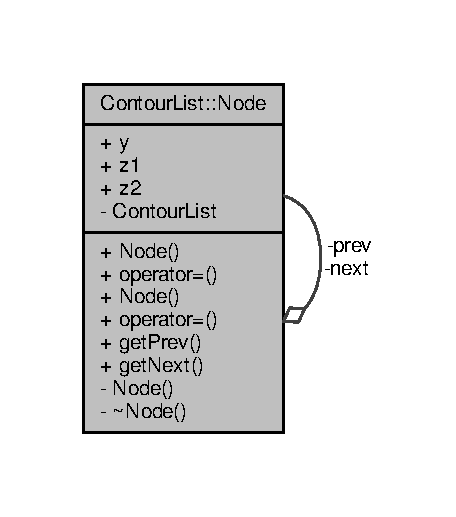
\includegraphics[width=222pt]{structContourList_1_1Node__coll__graph}
\end{center}
\end{figure}
\subsection*{Public Member Functions}
\begin{DoxyCompactItemize}
\item 
\hyperlink{structContourList_1_1Node_ac4e773feed1974871bd67d8d9575d3b9}{Node} (double \+\_\+y, double \+\_\+z1, double \+\_\+z2)
\begin{DoxyCompactList}\small\item\em prev-\/$>$z2 == z1, z2 == next-\/$>$z1 \end{DoxyCompactList}\item 
\hyperlink{structContourList_1_1Node_aa5a6173b45499956934fea3f0f988937}{Node} (const \hyperlink{structContourList_1_1Node}{Node} \&)=delete
\item 
\hyperlink{structContourList_1_1Node}{Node} \& \hyperlink{structContourList_1_1Node_a034f1203c181859eff8925b7f3549f37}{operator=} (const \hyperlink{structContourList_1_1Node}{Node} \&)=delete
\end{DoxyCompactItemize}
\subsection*{Public Attributes}
\begin{DoxyCompactItemize}
\item 
double \hyperlink{structContourList_1_1Node_ac371d90797c06c6b6a6de40e21d17110}{y}
\item 
double \hyperlink{structContourList_1_1Node_acf3193319486884386610f80a4681014}{z1}
\item 
double \hyperlink{structContourList_1_1Node_a5274d7d4c01c5205fb6dec2dd0065e11}{z2}
\item 
\hyperlink{structContourList_1_1Node}{Node} $\ast$ \hyperlink{structContourList_1_1Node_af08c22cbddfee4f0c0f6896c7284ed27}{prev}
\begin{DoxyCompactList}\small\item\em z1 $<$ z2 \end{DoxyCompactList}\item 
\hyperlink{structContourList_1_1Node}{Node} $\ast$ \hyperlink{structContourList_1_1Node_ab93d87ce30e069a1154bce37acf1964d}{next}
\end{DoxyCompactItemize}


\subsection{Detailed Description}
A node of a contour list. 

\subsection{Constructor \& Destructor Documentation}
\hypertarget{structContourList_1_1Node_ac4e773feed1974871bd67d8d9575d3b9}{}\index{Contour\+List\+::\+Node@{Contour\+List\+::\+Node}!Node@{Node}}
\index{Node@{Node}!Contour\+List\+::\+Node@{Contour\+List\+::\+Node}}
\subsubsection[{Node}]{\setlength{\rightskip}{0pt plus 5cm}Contour\+List\+::\+Node\+::\+Node (
\begin{DoxyParamCaption}
\item[{double}]{\+\_\+y, }
\item[{double}]{\+\_\+z1, }
\item[{double}]{\+\_\+z2}
\end{DoxyParamCaption}
)\hspace{0.3cm}{\ttfamily [inline]}}\label{structContourList_1_1Node_ac4e773feed1974871bd67d8d9575d3b9}


prev-\/$>$z2 == z1, z2 == next-\/$>$z1 

\hypertarget{structContourList_1_1Node_aa5a6173b45499956934fea3f0f988937}{}\index{Contour\+List\+::\+Node@{Contour\+List\+::\+Node}!Node@{Node}}
\index{Node@{Node}!Contour\+List\+::\+Node@{Contour\+List\+::\+Node}}
\subsubsection[{Node}]{\setlength{\rightskip}{0pt plus 5cm}Contour\+List\+::\+Node\+::\+Node (
\begin{DoxyParamCaption}
\item[{const {\bf Node} \&}]{}
\end{DoxyParamCaption}
)\hspace{0.3cm}{\ttfamily [delete]}}\label{structContourList_1_1Node_aa5a6173b45499956934fea3f0f988937}


\subsection{Member Function Documentation}
\hypertarget{structContourList_1_1Node_a034f1203c181859eff8925b7f3549f37}{}\index{Contour\+List\+::\+Node@{Contour\+List\+::\+Node}!operator=@{operator=}}
\index{operator=@{operator=}!Contour\+List\+::\+Node@{Contour\+List\+::\+Node}}
\subsubsection[{operator=}]{\setlength{\rightskip}{0pt plus 5cm}{\bf Node}\& Contour\+List\+::\+Node\+::operator= (
\begin{DoxyParamCaption}
\item[{const {\bf Node} \&}]{}
\end{DoxyParamCaption}
)\hspace{0.3cm}{\ttfamily [delete]}}\label{structContourList_1_1Node_a034f1203c181859eff8925b7f3549f37}


\subsection{Member Data Documentation}
\hypertarget{structContourList_1_1Node_ab93d87ce30e069a1154bce37acf1964d}{}\index{Contour\+List\+::\+Node@{Contour\+List\+::\+Node}!next@{next}}
\index{next@{next}!Contour\+List\+::\+Node@{Contour\+List\+::\+Node}}
\subsubsection[{next}]{\setlength{\rightskip}{0pt plus 5cm}{\bf Node} $\ast$ Contour\+List\+::\+Node\+::next}\label{structContourList_1_1Node_ab93d87ce30e069a1154bce37acf1964d}
\hypertarget{structContourList_1_1Node_af08c22cbddfee4f0c0f6896c7284ed27}{}\index{Contour\+List\+::\+Node@{Contour\+List\+::\+Node}!prev@{prev}}
\index{prev@{prev}!Contour\+List\+::\+Node@{Contour\+List\+::\+Node}}
\subsubsection[{prev}]{\setlength{\rightskip}{0pt plus 5cm}{\bf Node}$\ast$ Contour\+List\+::\+Node\+::prev}\label{structContourList_1_1Node_af08c22cbddfee4f0c0f6896c7284ed27}


z1 $<$ z2 

\hypertarget{structContourList_1_1Node_ac371d90797c06c6b6a6de40e21d17110}{}\index{Contour\+List\+::\+Node@{Contour\+List\+::\+Node}!y@{y}}
\index{y@{y}!Contour\+List\+::\+Node@{Contour\+List\+::\+Node}}
\subsubsection[{y}]{\setlength{\rightskip}{0pt plus 5cm}double Contour\+List\+::\+Node\+::y}\label{structContourList_1_1Node_ac371d90797c06c6b6a6de40e21d17110}
\hypertarget{structContourList_1_1Node_acf3193319486884386610f80a4681014}{}\index{Contour\+List\+::\+Node@{Contour\+List\+::\+Node}!z1@{z1}}
\index{z1@{z1}!Contour\+List\+::\+Node@{Contour\+List\+::\+Node}}
\subsubsection[{z1}]{\setlength{\rightskip}{0pt plus 5cm}double Contour\+List\+::\+Node\+::z1}\label{structContourList_1_1Node_acf3193319486884386610f80a4681014}
\hypertarget{structContourList_1_1Node_a5274d7d4c01c5205fb6dec2dd0065e11}{}\index{Contour\+List\+::\+Node@{Contour\+List\+::\+Node}!z2@{z2}}
\index{z2@{z2}!Contour\+List\+::\+Node@{Contour\+List\+::\+Node}}
\subsubsection[{z2}]{\setlength{\rightskip}{0pt plus 5cm}double Contour\+List\+::\+Node\+::z2}\label{structContourList_1_1Node_a5274d7d4c01c5205fb6dec2dd0065e11}


The documentation for this struct was generated from the following file\+:\begin{DoxyCompactItemize}
\item 
\hyperlink{ContourList_8h}{Contour\+List.\+h}\end{DoxyCompactItemize}

\hypertarget{classPlacement}{}\section{Placement Class Reference}
\label{classPlacement}\index{Placement@{Placement}}


A compact placement of blocks.  




{\ttfamily \#include $<$Placement.\+h$>$}



Collaboration diagram for Placement\+:
\nopagebreak
\begin{figure}[H]
\begin{center}
\leavevmode
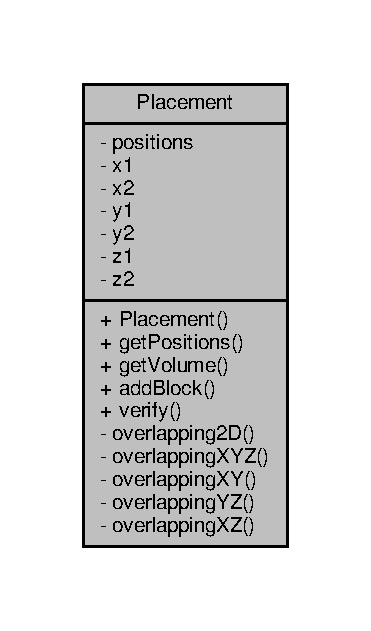
\includegraphics[width=178pt]{classPlacement__coll__graph}
\end{center}
\end{figure}
\subsection*{Classes}
\begin{DoxyCompactItemize}
\item 
struct \hyperlink{structPlacement_1_1BlockWithPos}{Block\+With\+Pos}
\end{DoxyCompactItemize}
\subsection*{Public Member Functions}
\begin{DoxyCompactItemize}
\item 
\hyperlink{classPlacement_aa0020a3dd0bedb34998968adfacf8a4e}{Placement} ()
\item 
const std\+::vector$<$ \hyperlink{structPlacement_1_1BlockWithPos}{Block\+With\+Pos} $>$ \& \hyperlink{classPlacement_a8d2aff015fbf652bbccae2db6c7dd7d9}{get\+Positions} () const 
\begin{DoxyCompactList}\small\item\em Get all blocks\textquotesingle{} positions. \end{DoxyCompactList}\item 
double \hyperlink{classPlacement_a686b1f2aa26ae12285a5759d1b6e5f67}{get\+Volume} () const 
\begin{DoxyCompactList}\small\item\em Get the volume of the bounding box. \end{DoxyCompactList}\item 
double \hyperlink{classPlacement_a479626954e228086398665507bed9beb}{get\+Net\+Volume} () const 
\begin{DoxyCompactList}\small\item\em Get total volume of every blocks. \end{DoxyCompactList}\item 
void \hyperlink{classPlacement_a21dc44cf496d771e5c2ac17a24ac1703}{add\+Block} (const \hyperlink{structRotatableBlock}{Rotatable\+Block} \&\+\_\+block, double \+\_\+y, double \+\_\+z)
\begin{DoxyCompactList}\small\item\em Add one block into this placement. \end{DoxyCompactList}\item 
void \hyperlink{classPlacement_a7e54624dff8703581efc6be7d1af991e}{verify} () const 
\begin{DoxyCompactList}\small\item\em Verify some correctness. \end{DoxyCompactList}\end{DoxyCompactItemize}
\subsection*{Static Private Member Functions}
\begin{DoxyCompactItemize}
\item 
static bool \hyperlink{classPlacement_a9d95d0c91c23c7c8d627a81ed03ffa13}{overlapping2\+D} (double \hyperlink{classPlacement_a4c17ed499418886700bf8e4d4ee45047}{y1}, double \hyperlink{classPlacement_a3e9d90f2d85b6641d2fd7d74d2600394}{z1}, double w1, double h1, double \hyperlink{classPlacement_ae7b89409ab130ba3d7c268faf7175b40}{y2}, double \hyperlink{classPlacement_aed710205286315a2a14f8cc2ceacd267}{z2}, double w2, double h2)
\begin{DoxyCompactList}\small\item\em Check whether two squres are overlapping with each other in 2\+D plane (parameters for Y\+Z plane) \end{DoxyCompactList}\item 
static bool \hyperlink{classPlacement_aedd3513c4fc7a9cccd83144c65c83c00}{overlapping\+X\+Y\+Z} (const \hyperlink{structPlacement_1_1BlockWithPos}{Block\+With\+Pos} \&b1, const \hyperlink{structPlacement_1_1BlockWithPos}{Block\+With\+Pos} \&b2)
\begin{DoxyCompactList}\small\item\em Check whether two \hyperlink{structPlacement_1_1BlockWithPos}{Placement\+::\+Block\+With\+Pos} are overlapping with each other. \end{DoxyCompactList}\item 
static bool \hyperlink{classPlacement_ab87e46b2e8e64fd0be0c07b74651cd82}{overlapping\+X\+Y} (const \hyperlink{structPlacement_1_1BlockWithPos}{Block\+With\+Pos} \&b1, const \hyperlink{structPlacement_1_1BlockWithPos}{Block\+With\+Pos} \&b2)
\item 
static bool \hyperlink{classPlacement_a2f0b907f20632d98c1169e7c3ad427db}{overlapping\+Y\+Z} (const \hyperlink{structPlacement_1_1BlockWithPos}{Block\+With\+Pos} \&b1, const \hyperlink{structPlacement_1_1BlockWithPos}{Block\+With\+Pos} \&b2)
\item 
static bool \hyperlink{classPlacement_af6823b9b781ae186e922774bb4623b17}{overlapping\+X\+Z} (const \hyperlink{structPlacement_1_1BlockWithPos}{Block\+With\+Pos} \&b1, const \hyperlink{structPlacement_1_1BlockWithPos}{Block\+With\+Pos} \&b2)
\end{DoxyCompactItemize}
\subsection*{Private Attributes}
\begin{DoxyCompactItemize}
\item 
std\+::vector$<$ \hyperlink{structPlacement_1_1BlockWithPos}{Block\+With\+Pos} $>$ \hyperlink{classPlacement_a5c4c9527336f2c2c18e2c6234aad8878}{positions}
\item 
double \hyperlink{classPlacement_a7061408d3dac137528697314b5825daf}{x1}
\begin{DoxyCompactList}\small\item\em Six boundary. \end{DoxyCompactList}\item 
double \hyperlink{classPlacement_acb44c4ead672e30af3b6cf3758db090c}{x2}
\item 
double \hyperlink{classPlacement_a4c17ed499418886700bf8e4d4ee45047}{y1}
\item 
double \hyperlink{classPlacement_ae7b89409ab130ba3d7c268faf7175b40}{y2}
\item 
double \hyperlink{classPlacement_a3e9d90f2d85b6641d2fd7d74d2600394}{z1}
\item 
double \hyperlink{classPlacement_aed710205286315a2a14f8cc2ceacd267}{z2}
\item 
double \hyperlink{classPlacement_afe51f89ddfdb2d27b68449d96f50e24d}{net\+Volume}
\begin{DoxyCompactList}\small\item\em Total volume of every blocks. \end{DoxyCompactList}\end{DoxyCompactItemize}
\subsection*{Static Private Attributes}
\begin{DoxyCompactItemize}
\item 
static constexpr const double \hyperlink{classPlacement_a8af99bcb7758493e48ac8270023f96d7}{eps} = 1e-\/7
\begin{DoxyCompactList}\small\item\em Error tolerance. \end{DoxyCompactList}\end{DoxyCompactItemize}


\subsection{Detailed Description}
A compact placement of blocks. 

Difference $<$ 1e-\/7 will be considered as error 

\subsection{Constructor \& Destructor Documentation}
\hypertarget{classPlacement_aa0020a3dd0bedb34998968adfacf8a4e}{}\index{Placement@{Placement}!Placement@{Placement}}
\index{Placement@{Placement}!Placement@{Placement}}
\subsubsection[{Placement}]{\setlength{\rightskip}{0pt plus 5cm}Placement\+::\+Placement (
\begin{DoxyParamCaption}
{}
\end{DoxyParamCaption}
)\hspace{0.3cm}{\ttfamily [inline]}}\label{classPlacement_aa0020a3dd0bedb34998968adfacf8a4e}


\subsection{Member Function Documentation}
\hypertarget{classPlacement_a21dc44cf496d771e5c2ac17a24ac1703}{}\index{Placement@{Placement}!add\+Block@{add\+Block}}
\index{add\+Block@{add\+Block}!Placement@{Placement}}
\subsubsection[{add\+Block}]{\setlength{\rightskip}{0pt plus 5cm}void Placement\+::add\+Block (
\begin{DoxyParamCaption}
\item[{const {\bf Rotatable\+Block} \&}]{\+\_\+block, }
\item[{double}]{\+\_\+y, }
\item[{double}]{\+\_\+z}
\end{DoxyParamCaption}
)}\label{classPlacement_a21dc44cf496d771e5c2ac17a24ac1703}


Add one block into this placement. 

\hypertarget{classPlacement_a479626954e228086398665507bed9beb}{}\index{Placement@{Placement}!get\+Net\+Volume@{get\+Net\+Volume}}
\index{get\+Net\+Volume@{get\+Net\+Volume}!Placement@{Placement}}
\subsubsection[{get\+Net\+Volume}]{\setlength{\rightskip}{0pt plus 5cm}double Placement\+::get\+Net\+Volume (
\begin{DoxyParamCaption}
{}
\end{DoxyParamCaption}
) const\hspace{0.3cm}{\ttfamily [inline]}}\label{classPlacement_a479626954e228086398665507bed9beb}


Get total volume of every blocks. 

\hypertarget{classPlacement_a8d2aff015fbf652bbccae2db6c7dd7d9}{}\index{Placement@{Placement}!get\+Positions@{get\+Positions}}
\index{get\+Positions@{get\+Positions}!Placement@{Placement}}
\subsubsection[{get\+Positions}]{\setlength{\rightskip}{0pt plus 5cm}const std\+::vector$<${\bf Block\+With\+Pos}$>$\& Placement\+::get\+Positions (
\begin{DoxyParamCaption}
{}
\end{DoxyParamCaption}
) const\hspace{0.3cm}{\ttfamily [inline]}}\label{classPlacement_a8d2aff015fbf652bbccae2db6c7dd7d9}


Get all blocks\textquotesingle{} positions. 

\hypertarget{classPlacement_a686b1f2aa26ae12285a5759d1b6e5f67}{}\index{Placement@{Placement}!get\+Volume@{get\+Volume}}
\index{get\+Volume@{get\+Volume}!Placement@{Placement}}
\subsubsection[{get\+Volume}]{\setlength{\rightskip}{0pt plus 5cm}double Placement\+::get\+Volume (
\begin{DoxyParamCaption}
{}
\end{DoxyParamCaption}
) const\hspace{0.3cm}{\ttfamily [inline]}}\label{classPlacement_a686b1f2aa26ae12285a5759d1b6e5f67}


Get the volume of the bounding box. 

\hypertarget{classPlacement_a9d95d0c91c23c7c8d627a81ed03ffa13}{}\index{Placement@{Placement}!overlapping2\+D@{overlapping2\+D}}
\index{overlapping2\+D@{overlapping2\+D}!Placement@{Placement}}
\subsubsection[{overlapping2\+D}]{\setlength{\rightskip}{0pt plus 5cm}bool Placement\+::overlapping2\+D (
\begin{DoxyParamCaption}
\item[{double}]{y1, }
\item[{double}]{z1, }
\item[{double}]{w1, }
\item[{double}]{h1, }
\item[{double}]{y2, }
\item[{double}]{z2, }
\item[{double}]{w2, }
\item[{double}]{h2}
\end{DoxyParamCaption}
)\hspace{0.3cm}{\ttfamily [inline]}, {\ttfamily [static]}, {\ttfamily [private]}}\label{classPlacement_a9d95d0c91c23c7c8d627a81ed03ffa13}


Check whether two squres are overlapping with each other in 2\+D plane (parameters for Y\+Z plane) 

\hypertarget{classPlacement_ab87e46b2e8e64fd0be0c07b74651cd82}{}\index{Placement@{Placement}!overlapping\+X\+Y@{overlapping\+X\+Y}}
\index{overlapping\+X\+Y@{overlapping\+X\+Y}!Placement@{Placement}}
\subsubsection[{overlapping\+X\+Y}]{\setlength{\rightskip}{0pt plus 5cm}bool Placement\+::overlapping\+X\+Y (
\begin{DoxyParamCaption}
\item[{const {\bf Block\+With\+Pos} \&}]{b1, }
\item[{const {\bf Block\+With\+Pos} \&}]{b2}
\end{DoxyParamCaption}
)\hspace{0.3cm}{\ttfamily [inline]}, {\ttfamily [static]}, {\ttfamily [private]}}\label{classPlacement_ab87e46b2e8e64fd0be0c07b74651cd82}
\hypertarget{classPlacement_aedd3513c4fc7a9cccd83144c65c83c00}{}\index{Placement@{Placement}!overlapping\+X\+Y\+Z@{overlapping\+X\+Y\+Z}}
\index{overlapping\+X\+Y\+Z@{overlapping\+X\+Y\+Z}!Placement@{Placement}}
\subsubsection[{overlapping\+X\+Y\+Z}]{\setlength{\rightskip}{0pt plus 5cm}bool Placement\+::overlapping\+X\+Y\+Z (
\begin{DoxyParamCaption}
\item[{const {\bf Block\+With\+Pos} \&}]{b1, }
\item[{const {\bf Block\+With\+Pos} \&}]{b2}
\end{DoxyParamCaption}
)\hspace{0.3cm}{\ttfamily [inline]}, {\ttfamily [static]}, {\ttfamily [private]}}\label{classPlacement_aedd3513c4fc7a9cccd83144c65c83c00}


Check whether two \hyperlink{structPlacement_1_1BlockWithPos}{Placement\+::\+Block\+With\+Pos} are overlapping with each other. 

\hypertarget{classPlacement_af6823b9b781ae186e922774bb4623b17}{}\index{Placement@{Placement}!overlapping\+X\+Z@{overlapping\+X\+Z}}
\index{overlapping\+X\+Z@{overlapping\+X\+Z}!Placement@{Placement}}
\subsubsection[{overlapping\+X\+Z}]{\setlength{\rightskip}{0pt plus 5cm}bool Placement\+::overlapping\+X\+Z (
\begin{DoxyParamCaption}
\item[{const {\bf Block\+With\+Pos} \&}]{b1, }
\item[{const {\bf Block\+With\+Pos} \&}]{b2}
\end{DoxyParamCaption}
)\hspace{0.3cm}{\ttfamily [inline]}, {\ttfamily [static]}, {\ttfamily [private]}}\label{classPlacement_af6823b9b781ae186e922774bb4623b17}
\hypertarget{classPlacement_a2f0b907f20632d98c1169e7c3ad427db}{}\index{Placement@{Placement}!overlapping\+Y\+Z@{overlapping\+Y\+Z}}
\index{overlapping\+Y\+Z@{overlapping\+Y\+Z}!Placement@{Placement}}
\subsubsection[{overlapping\+Y\+Z}]{\setlength{\rightskip}{0pt plus 5cm}bool Placement\+::overlapping\+Y\+Z (
\begin{DoxyParamCaption}
\item[{const {\bf Block\+With\+Pos} \&}]{b1, }
\item[{const {\bf Block\+With\+Pos} \&}]{b2}
\end{DoxyParamCaption}
)\hspace{0.3cm}{\ttfamily [inline]}, {\ttfamily [static]}, {\ttfamily [private]}}\label{classPlacement_a2f0b907f20632d98c1169e7c3ad427db}
\hypertarget{classPlacement_a7e54624dff8703581efc6be7d1af991e}{}\index{Placement@{Placement}!verify@{verify}}
\index{verify@{verify}!Placement@{Placement}}
\subsubsection[{verify}]{\setlength{\rightskip}{0pt plus 5cm}void Placement\+::verify (
\begin{DoxyParamCaption}
{}
\end{DoxyParamCaption}
) const}\label{classPlacement_a7e54624dff8703581efc6be7d1af991e}


Verify some correctness. 



\subsection{Member Data Documentation}
\hypertarget{classPlacement_a8af99bcb7758493e48ac8270023f96d7}{}\index{Placement@{Placement}!eps@{eps}}
\index{eps@{eps}!Placement@{Placement}}
\subsubsection[{eps}]{\setlength{\rightskip}{0pt plus 5cm}constexpr const double Placement\+::eps = 1e-\/7\hspace{0.3cm}{\ttfamily [static]}, {\ttfamily [private]}}\label{classPlacement_a8af99bcb7758493e48ac8270023f96d7}


Error tolerance. 

\hypertarget{classPlacement_afe51f89ddfdb2d27b68449d96f50e24d}{}\index{Placement@{Placement}!net\+Volume@{net\+Volume}}
\index{net\+Volume@{net\+Volume}!Placement@{Placement}}
\subsubsection[{net\+Volume}]{\setlength{\rightskip}{0pt plus 5cm}double Placement\+::net\+Volume\hspace{0.3cm}{\ttfamily [private]}}\label{classPlacement_afe51f89ddfdb2d27b68449d96f50e24d}


Total volume of every blocks. 

\hypertarget{classPlacement_a5c4c9527336f2c2c18e2c6234aad8878}{}\index{Placement@{Placement}!positions@{positions}}
\index{positions@{positions}!Placement@{Placement}}
\subsubsection[{positions}]{\setlength{\rightskip}{0pt plus 5cm}std\+::vector$<${\bf Block\+With\+Pos}$>$ Placement\+::positions\hspace{0.3cm}{\ttfamily [private]}}\label{classPlacement_a5c4c9527336f2c2c18e2c6234aad8878}
\hypertarget{classPlacement_a7061408d3dac137528697314b5825daf}{}\index{Placement@{Placement}!x1@{x1}}
\index{x1@{x1}!Placement@{Placement}}
\subsubsection[{x1}]{\setlength{\rightskip}{0pt plus 5cm}double Placement\+::x1\hspace{0.3cm}{\ttfamily [private]}}\label{classPlacement_a7061408d3dac137528697314b5825daf}


Six boundary. 

\hypertarget{classPlacement_acb44c4ead672e30af3b6cf3758db090c}{}\index{Placement@{Placement}!x2@{x2}}
\index{x2@{x2}!Placement@{Placement}}
\subsubsection[{x2}]{\setlength{\rightskip}{0pt plus 5cm}double Placement\+::x2\hspace{0.3cm}{\ttfamily [private]}}\label{classPlacement_acb44c4ead672e30af3b6cf3758db090c}
\hypertarget{classPlacement_a4c17ed499418886700bf8e4d4ee45047}{}\index{Placement@{Placement}!y1@{y1}}
\index{y1@{y1}!Placement@{Placement}}
\subsubsection[{y1}]{\setlength{\rightskip}{0pt plus 5cm}double Placement\+::y1\hspace{0.3cm}{\ttfamily [private]}}\label{classPlacement_a4c17ed499418886700bf8e4d4ee45047}
\hypertarget{classPlacement_ae7b89409ab130ba3d7c268faf7175b40}{}\index{Placement@{Placement}!y2@{y2}}
\index{y2@{y2}!Placement@{Placement}}
\subsubsection[{y2}]{\setlength{\rightskip}{0pt plus 5cm}double Placement\+::y2\hspace{0.3cm}{\ttfamily [private]}}\label{classPlacement_ae7b89409ab130ba3d7c268faf7175b40}
\hypertarget{classPlacement_a3e9d90f2d85b6641d2fd7d74d2600394}{}\index{Placement@{Placement}!z1@{z1}}
\index{z1@{z1}!Placement@{Placement}}
\subsubsection[{z1}]{\setlength{\rightskip}{0pt plus 5cm}double Placement\+::z1\hspace{0.3cm}{\ttfamily [private]}}\label{classPlacement_a3e9d90f2d85b6641d2fd7d74d2600394}
\hypertarget{classPlacement_aed710205286315a2a14f8cc2ceacd267}{}\index{Placement@{Placement}!z2@{z2}}
\index{z2@{z2}!Placement@{Placement}}
\subsubsection[{z2}]{\setlength{\rightskip}{0pt plus 5cm}double Placement\+::z2\hspace{0.3cm}{\ttfamily [private]}}\label{classPlacement_aed710205286315a2a14f8cc2ceacd267}


The documentation for this class was generated from the following files\+:\begin{DoxyCompactItemize}
\item 
\hyperlink{Placement_8h}{Placement.\+h}\item 
\hyperlink{Placement_8cpp}{Placement.\+cpp}\end{DoxyCompactItemize}

\hypertarget{classRandom}{}\section{Random Class Reference}
\label{classRandom}\index{Random@{Random}}


Please to this file instead of generate random numbers by yourself. It provide a consistent control of the seed.  




{\ttfamily \#include $<$Random.\+h$>$}



Collaboration diagram for Random\+:\nopagebreak
\begin{figure}[H]
\begin{center}
\leavevmode
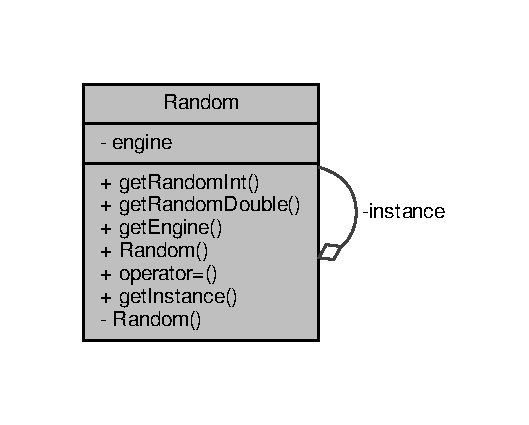
\includegraphics[width=254pt]{classRandom__coll__graph}
\end{center}
\end{figure}
\subsection*{Public Types}
\begin{DoxyCompactItemize}
\item 
typedef std\+::default\+\_\+random\+\_\+engine \hyperlink{classRandom_ab1090b767f3e771eb8f846079869d1b4}{engine\+\_\+t}
\begin{DoxyCompactList}\small\item\em You can change this to other engines. \end{DoxyCompactList}\end{DoxyCompactItemize}
\subsection*{Public Member Functions}
\begin{DoxyCompactItemize}
\item 
int \hyperlink{classRandom_a7365696fe6cb07dc6c686bfde4fbf4ae}{get\+Random\+Int} (int lo, int hi)
\begin{DoxyCompactList}\small\item\em Generate random integer in \mbox{[}lo,hi\mbox{]}. \end{DoxyCompactList}\item 
double \hyperlink{classRandom_a721d558ed4bf72c63ceec816c5819129}{get\+Random\+Double} (double lo, double hi)
\begin{DoxyCompactList}\small\item\em Generate random real in \mbox{[}lo, hi\mbox{]}. \end{DoxyCompactList}\item 
\hyperlink{classRandom_ab1090b767f3e771eb8f846079869d1b4}{engine\+\_\+t} \& \hyperlink{classRandom_aa4b65c7cd8e0ada6c0dca5937236dda0}{get\+Engine} ()
\begin{DoxyCompactList}\small\item\em Get random engine. \end{DoxyCompactList}\item 
\hyperlink{classRandom_a9bfadeaa4adc5ac44142d000b1c99441}{Random} (const \hyperlink{classRandom}{Random} \&)=delete
\item 
\hyperlink{classRandom}{Random} \& \hyperlink{classRandom_acc7a4d85a416a090cde22c9273e01f1e}{operator=} (const \hyperlink{classRandom}{Random} \&)=delete
\end{DoxyCompactItemize}
\subsection*{Static Public Member Functions}
\begin{DoxyCompactItemize}
\item 
static \hyperlink{classRandom}{Random} \& \hyperlink{classRandom_a2aa30d2f678fc76f75efc60356c6ea4d}{get\+Instance} ()
\end{DoxyCompactItemize}
\subsection*{Private Member Functions}
\begin{DoxyCompactItemize}
\item 
\hyperlink{classRandom_acb76b49c3903a3c4fb67fd216341f08d}{Random} ()
\end{DoxyCompactItemize}
\subsection*{Private Attributes}
\begin{DoxyCompactItemize}
\item 
\hyperlink{classRandom_ab1090b767f3e771eb8f846079869d1b4}{engine\+\_\+t} \hyperlink{classRandom_a273901a5b482668a1a0204b8691317e1}{engine}
\end{DoxyCompactItemize}
\subsection*{Static Private Attributes}
\begin{DoxyCompactItemize}
\item 
static \hyperlink{classRandom}{Random} $\ast$ \hyperlink{classRandom_a841a26400e4205f27cfb1ab4acaccb46}{instance} = N\+U\+L\+L
\end{DoxyCompactItemize}


\subsection{Detailed Description}
Please to this file instead of generate random numbers by yourself. It provide a consistent control of the seed. 

\hyperlink{classRandom}{Random} number generator. Define N\+D\+E\+B\+U\+G to enable generating seed accroding to time. 

\subsection{Member Typedef Documentation}
\hypertarget{classRandom_ab1090b767f3e771eb8f846079869d1b4}{}\index{Random@{Random}!engine\+\_\+t@{engine\+\_\+t}}
\index{engine\+\_\+t@{engine\+\_\+t}!Random@{Random}}
\subsubsection[{engine\+\_\+t}]{\setlength{\rightskip}{0pt plus 5cm}typedef std\+::default\+\_\+random\+\_\+engine {\bf Random\+::engine\+\_\+t}}\label{classRandom_ab1090b767f3e771eb8f846079869d1b4}


You can change this to other engines. 



\subsection{Constructor \& Destructor Documentation}
\hypertarget{classRandom_a9bfadeaa4adc5ac44142d000b1c99441}{}\index{Random@{Random}!Random@{Random}}
\index{Random@{Random}!Random@{Random}}
\subsubsection[{Random}]{\setlength{\rightskip}{0pt plus 5cm}Random\+::\+Random (
\begin{DoxyParamCaption}
\item[{const {\bf Random} \&}]{}
\end{DoxyParamCaption}
)\hspace{0.3cm}{\ttfamily [delete]}}\label{classRandom_a9bfadeaa4adc5ac44142d000b1c99441}
\hypertarget{classRandom_acb76b49c3903a3c4fb67fd216341f08d}{}\index{Random@{Random}!Random@{Random}}
\index{Random@{Random}!Random@{Random}}
\subsubsection[{Random}]{\setlength{\rightskip}{0pt plus 5cm}Random\+::\+Random (
\begin{DoxyParamCaption}
{}
\end{DoxyParamCaption}
)\hspace{0.3cm}{\ttfamily [private]}}\label{classRandom_acb76b49c3903a3c4fb67fd216341f08d}


\subsection{Member Function Documentation}
\hypertarget{classRandom_aa4b65c7cd8e0ada6c0dca5937236dda0}{}\index{Random@{Random}!get\+Engine@{get\+Engine}}
\index{get\+Engine@{get\+Engine}!Random@{Random}}
\subsubsection[{get\+Engine}]{\setlength{\rightskip}{0pt plus 5cm}{\bf engine\+\_\+t}\& Random\+::get\+Engine (
\begin{DoxyParamCaption}
{}
\end{DoxyParamCaption}
)\hspace{0.3cm}{\ttfamily [inline]}}\label{classRandom_aa4b65c7cd8e0ada6c0dca5937236dda0}


Get random engine. 

\hypertarget{classRandom_a2aa30d2f678fc76f75efc60356c6ea4d}{}\index{Random@{Random}!get\+Instance@{get\+Instance}}
\index{get\+Instance@{get\+Instance}!Random@{Random}}
\subsubsection[{get\+Instance}]{\setlength{\rightskip}{0pt plus 5cm}{\bf Random} \& Random\+::get\+Instance (
\begin{DoxyParamCaption}
{}
\end{DoxyParamCaption}
)\hspace{0.3cm}{\ttfamily [inline]}, {\ttfamily [static]}}\label{classRandom_a2aa30d2f678fc76f75efc60356c6ea4d}
\hypertarget{classRandom_a721d558ed4bf72c63ceec816c5819129}{}\index{Random@{Random}!get\+Random\+Double@{get\+Random\+Double}}
\index{get\+Random\+Double@{get\+Random\+Double}!Random@{Random}}
\subsubsection[{get\+Random\+Double}]{\setlength{\rightskip}{0pt plus 5cm}double Random\+::get\+Random\+Double (
\begin{DoxyParamCaption}
\item[{double}]{lo, }
\item[{double}]{hi}
\end{DoxyParamCaption}
)\hspace{0.3cm}{\ttfamily [inline]}}\label{classRandom_a721d558ed4bf72c63ceec816c5819129}


Generate random real in \mbox{[}lo, hi\mbox{]}. 

\hypertarget{classRandom_a7365696fe6cb07dc6c686bfde4fbf4ae}{}\index{Random@{Random}!get\+Random\+Int@{get\+Random\+Int}}
\index{get\+Random\+Int@{get\+Random\+Int}!Random@{Random}}
\subsubsection[{get\+Random\+Int}]{\setlength{\rightskip}{0pt plus 5cm}int Random\+::get\+Random\+Int (
\begin{DoxyParamCaption}
\item[{int}]{lo, }
\item[{int}]{hi}
\end{DoxyParamCaption}
)\hspace{0.3cm}{\ttfamily [inline]}}\label{classRandom_a7365696fe6cb07dc6c686bfde4fbf4ae}


Generate random integer in \mbox{[}lo,hi\mbox{]}. 

\hypertarget{classRandom_acc7a4d85a416a090cde22c9273e01f1e}{}\index{Random@{Random}!operator=@{operator=}}
\index{operator=@{operator=}!Random@{Random}}
\subsubsection[{operator=}]{\setlength{\rightskip}{0pt plus 5cm}{\bf Random}\& Random\+::operator= (
\begin{DoxyParamCaption}
\item[{const {\bf Random} \&}]{}
\end{DoxyParamCaption}
)\hspace{0.3cm}{\ttfamily [delete]}}\label{classRandom_acc7a4d85a416a090cde22c9273e01f1e}


\subsection{Member Data Documentation}
\hypertarget{classRandom_a273901a5b482668a1a0204b8691317e1}{}\index{Random@{Random}!engine@{engine}}
\index{engine@{engine}!Random@{Random}}
\subsubsection[{engine}]{\setlength{\rightskip}{0pt plus 5cm}{\bf engine\+\_\+t} Random\+::engine\hspace{0.3cm}{\ttfamily [private]}}\label{classRandom_a273901a5b482668a1a0204b8691317e1}
\hypertarget{classRandom_a841a26400e4205f27cfb1ab4acaccb46}{}\index{Random@{Random}!instance@{instance}}
\index{instance@{instance}!Random@{Random}}
\subsubsection[{instance}]{\setlength{\rightskip}{0pt plus 5cm}{\bf Random} $\ast$ Random\+::instance = N\+U\+L\+L\hspace{0.3cm}{\ttfamily [static]}, {\ttfamily [private]}}\label{classRandom_a841a26400e4205f27cfb1ab4acaccb46}


The documentation for this class was generated from the following files\+:\begin{DoxyCompactItemize}
\item 
\hyperlink{Random_8h}{Random.\+h}\item 
\hyperlink{Random_8cpp}{Random.\+cpp}\end{DoxyCompactItemize}

\hypertarget{structRotatableBlock}{}\section{Rotatable\+Block Struct Reference}
\label{structRotatableBlock}\index{Rotatable\+Block@{Rotatable\+Block}}


{\ttfamily \#include $<$Block.\+h$>$}



Collaboration diagram for Rotatable\+Block\+:\nopagebreak
\begin{figure}[H]
\begin{center}
\leavevmode
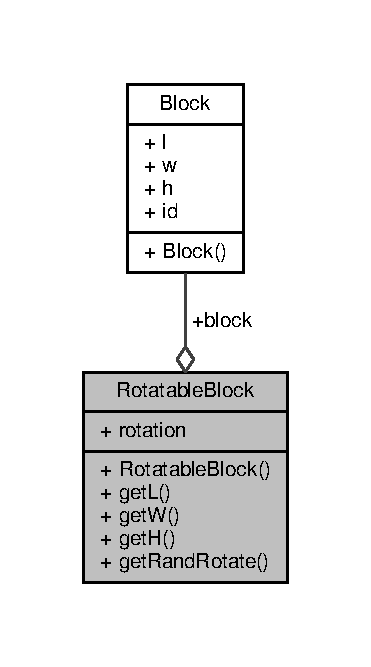
\includegraphics[width=178pt]{structRotatableBlock__coll__graph}
\end{center}
\end{figure}
\subsection*{Public Types}
\begin{DoxyCompactItemize}
\item 
enum \hyperlink{structRotatableBlock_ac076f0b2a72673cd4a5da5ea53b2e465}{R\+O\+T\+A\+T\+E\+\_\+\+N\+A\+M\+E} \{ \\*
\hyperlink{structRotatableBlock_ac076f0b2a72673cd4a5da5ea53b2e465a4e5874dc7e7f4a793efd2b3abecb34c9}{X\+Y\+Z} = 0x012, 
\hyperlink{structRotatableBlock_ac076f0b2a72673cd4a5da5ea53b2e465a8accfa9f236c3d421cf1863035093346}{X\+Z\+Y} = 0x021, 
\hyperlink{structRotatableBlock_ac076f0b2a72673cd4a5da5ea53b2e465ad22b8f1162e159ff4a3137db9c1e34d0}{Y\+X\+Z} = 0x102, 
\hyperlink{structRotatableBlock_ac076f0b2a72673cd4a5da5ea53b2e465a930b4b7cd8e1df5745dc7a6a4bf2355e}{Y\+Z\+X} = 0x120, 
\\*
\hyperlink{structRotatableBlock_ac076f0b2a72673cd4a5da5ea53b2e465a0cd2dbb032ea58008adafa343d3e8111}{Z\+X\+Y} = 0x201, 
\hyperlink{structRotatableBlock_ac076f0b2a72673cd4a5da5ea53b2e465abae8fc51a17af85462aa1e971e379c17}{Z\+Y\+X} = 0x210
 \}
\begin{DoxyCompactList}\small\item\em Y\+Z\+X means w\textquotesingle{}=l, h\textquotesingle{}=w, l\textquotesingle{}=h. (l\textquotesingle{},w\textquotesingle{},h\textquotesingle{}) is current one. \end{DoxyCompactList}\end{DoxyCompactItemize}
\subsection*{Public Member Functions}
\begin{DoxyCompactItemize}
\item 
\hyperlink{structRotatableBlock_ac9c0dd6af399b054a0011332b0b7fa77}{Rotatable\+Block} (const \hyperlink{structBlock}{Block} $\ast$\+\_\+block, \hyperlink{structRotatableBlock_ac076f0b2a72673cd4a5da5ea53b2e465}{R\+O\+T\+A\+T\+E\+\_\+\+N\+A\+M\+E} \+\_\+rotation)
\item 
double \hyperlink{structRotatableBlock_a0ed9c1f491d20ef51f1a655bf9ebbb2f}{get\+L} () const 
\item 
double \hyperlink{structRotatableBlock_a7516433d41793095435f3e99ef88edae}{get\+W} () const 
\item 
double \hyperlink{structRotatableBlock_ac4f1a519af134049d68d9ee103c2aa89}{get\+H} () const 
\end{DoxyCompactItemize}
\subsection*{Static Public Member Functions}
\begin{DoxyCompactItemize}
\item 
static \hyperlink{structRotatableBlock_ac076f0b2a72673cd4a5da5ea53b2e465}{R\+O\+T\+A\+T\+E\+\_\+\+N\+A\+M\+E} \hyperlink{structRotatableBlock_a15b7b0840be5cd6f10e4acd89131cb2b}{get\+Rand\+Rotate} ()
\end{DoxyCompactItemize}
\subsection*{Public Attributes}
\begin{DoxyCompactItemize}
\item 
const \hyperlink{structBlock}{Block} $\ast$ \hyperlink{structRotatableBlock_a7ad9b648924d8c37caa80f44841be4c7}{block}
\item 
\hyperlink{structRotatableBlock_ac076f0b2a72673cd4a5da5ea53b2e465}{R\+O\+T\+A\+T\+E\+\_\+\+N\+A\+M\+E} \hyperlink{structRotatableBlock_a6aa97c762ffc8ad401459003a63e6cc0}{rotation}
\end{DoxyCompactItemize}


\subsection{Member Enumeration Documentation}
\hypertarget{structRotatableBlock_ac076f0b2a72673cd4a5da5ea53b2e465}{}\index{Rotatable\+Block@{Rotatable\+Block}!R\+O\+T\+A\+T\+E\+\_\+\+N\+A\+M\+E@{R\+O\+T\+A\+T\+E\+\_\+\+N\+A\+M\+E}}
\index{R\+O\+T\+A\+T\+E\+\_\+\+N\+A\+M\+E@{R\+O\+T\+A\+T\+E\+\_\+\+N\+A\+M\+E}!Rotatable\+Block@{Rotatable\+Block}}
\subsubsection[{R\+O\+T\+A\+T\+E\+\_\+\+N\+A\+M\+E}]{\setlength{\rightskip}{0pt plus 5cm}enum {\bf Rotatable\+Block\+::\+R\+O\+T\+A\+T\+E\+\_\+\+N\+A\+M\+E}}\label{structRotatableBlock_ac076f0b2a72673cd4a5da5ea53b2e465}


Y\+Z\+X means w\textquotesingle{}=l, h\textquotesingle{}=w, l\textquotesingle{}=h. (l\textquotesingle{},w\textquotesingle{},h\textquotesingle{}) is current one. 

\begin{Desc}
\item[Enumerator]\par
\begin{description}
\index{X\+Y\+Z@{X\+Y\+Z}!Rotatable\+Block@{Rotatable\+Block}}\index{Rotatable\+Block@{Rotatable\+Block}!X\+Y\+Z@{X\+Y\+Z}}\item[{\em 
\hypertarget{structRotatableBlock_ac076f0b2a72673cd4a5da5ea53b2e465a4e5874dc7e7f4a793efd2b3abecb34c9}{}X\+Y\+Z\label{structRotatableBlock_ac076f0b2a72673cd4a5da5ea53b2e465a4e5874dc7e7f4a793efd2b3abecb34c9}
}]\index{X\+Z\+Y@{X\+Z\+Y}!Rotatable\+Block@{Rotatable\+Block}}\index{Rotatable\+Block@{Rotatable\+Block}!X\+Z\+Y@{X\+Z\+Y}}\item[{\em 
\hypertarget{structRotatableBlock_ac076f0b2a72673cd4a5da5ea53b2e465a8accfa9f236c3d421cf1863035093346}{}X\+Z\+Y\label{structRotatableBlock_ac076f0b2a72673cd4a5da5ea53b2e465a8accfa9f236c3d421cf1863035093346}
}]\index{Y\+X\+Z@{Y\+X\+Z}!Rotatable\+Block@{Rotatable\+Block}}\index{Rotatable\+Block@{Rotatable\+Block}!Y\+X\+Z@{Y\+X\+Z}}\item[{\em 
\hypertarget{structRotatableBlock_ac076f0b2a72673cd4a5da5ea53b2e465ad22b8f1162e159ff4a3137db9c1e34d0}{}Y\+X\+Z\label{structRotatableBlock_ac076f0b2a72673cd4a5da5ea53b2e465ad22b8f1162e159ff4a3137db9c1e34d0}
}]\index{Y\+Z\+X@{Y\+Z\+X}!Rotatable\+Block@{Rotatable\+Block}}\index{Rotatable\+Block@{Rotatable\+Block}!Y\+Z\+X@{Y\+Z\+X}}\item[{\em 
\hypertarget{structRotatableBlock_ac076f0b2a72673cd4a5da5ea53b2e465a930b4b7cd8e1df5745dc7a6a4bf2355e}{}Y\+Z\+X\label{structRotatableBlock_ac076f0b2a72673cd4a5da5ea53b2e465a930b4b7cd8e1df5745dc7a6a4bf2355e}
}]\index{Z\+X\+Y@{Z\+X\+Y}!Rotatable\+Block@{Rotatable\+Block}}\index{Rotatable\+Block@{Rotatable\+Block}!Z\+X\+Y@{Z\+X\+Y}}\item[{\em 
\hypertarget{structRotatableBlock_ac076f0b2a72673cd4a5da5ea53b2e465a0cd2dbb032ea58008adafa343d3e8111}{}Z\+X\+Y\label{structRotatableBlock_ac076f0b2a72673cd4a5da5ea53b2e465a0cd2dbb032ea58008adafa343d3e8111}
}]\index{Z\+Y\+X@{Z\+Y\+X}!Rotatable\+Block@{Rotatable\+Block}}\index{Rotatable\+Block@{Rotatable\+Block}!Z\+Y\+X@{Z\+Y\+X}}\item[{\em 
\hypertarget{structRotatableBlock_ac076f0b2a72673cd4a5da5ea53b2e465abae8fc51a17af85462aa1e971e379c17}{}Z\+Y\+X\label{structRotatableBlock_ac076f0b2a72673cd4a5da5ea53b2e465abae8fc51a17af85462aa1e971e379c17}
}]\end{description}
\end{Desc}


\subsection{Constructor \& Destructor Documentation}
\hypertarget{structRotatableBlock_ac9c0dd6af399b054a0011332b0b7fa77}{}\index{Rotatable\+Block@{Rotatable\+Block}!Rotatable\+Block@{Rotatable\+Block}}
\index{Rotatable\+Block@{Rotatable\+Block}!Rotatable\+Block@{Rotatable\+Block}}
\subsubsection[{Rotatable\+Block}]{\setlength{\rightskip}{0pt plus 5cm}Rotatable\+Block\+::\+Rotatable\+Block (
\begin{DoxyParamCaption}
\item[{const {\bf Block} $\ast$}]{\+\_\+block, }
\item[{{\bf R\+O\+T\+A\+T\+E\+\_\+\+N\+A\+M\+E}}]{\+\_\+rotation}
\end{DoxyParamCaption}
)\hspace{0.3cm}{\ttfamily [inline]}}\label{structRotatableBlock_ac9c0dd6af399b054a0011332b0b7fa77}


\subsection{Member Function Documentation}
\hypertarget{structRotatableBlock_ac4f1a519af134049d68d9ee103c2aa89}{}\index{Rotatable\+Block@{Rotatable\+Block}!get\+H@{get\+H}}
\index{get\+H@{get\+H}!Rotatable\+Block@{Rotatable\+Block}}
\subsubsection[{get\+H}]{\setlength{\rightskip}{0pt plus 5cm}double Rotatable\+Block\+::get\+H (
\begin{DoxyParamCaption}
{}
\end{DoxyParamCaption}
) const\hspace{0.3cm}{\ttfamily [inline]}}\label{structRotatableBlock_ac4f1a519af134049d68d9ee103c2aa89}
\hypertarget{structRotatableBlock_a0ed9c1f491d20ef51f1a655bf9ebbb2f}{}\index{Rotatable\+Block@{Rotatable\+Block}!get\+L@{get\+L}}
\index{get\+L@{get\+L}!Rotatable\+Block@{Rotatable\+Block}}
\subsubsection[{get\+L}]{\setlength{\rightskip}{0pt plus 5cm}double Rotatable\+Block\+::get\+L (
\begin{DoxyParamCaption}
{}
\end{DoxyParamCaption}
) const\hspace{0.3cm}{\ttfamily [inline]}}\label{structRotatableBlock_a0ed9c1f491d20ef51f1a655bf9ebbb2f}
\hypertarget{structRotatableBlock_a15b7b0840be5cd6f10e4acd89131cb2b}{}\index{Rotatable\+Block@{Rotatable\+Block}!get\+Rand\+Rotate@{get\+Rand\+Rotate}}
\index{get\+Rand\+Rotate@{get\+Rand\+Rotate}!Rotatable\+Block@{Rotatable\+Block}}
\subsubsection[{get\+Rand\+Rotate}]{\setlength{\rightskip}{0pt plus 5cm}{\bf Rotatable\+Block\+::\+R\+O\+T\+A\+T\+E\+\_\+\+N\+A\+M\+E} Rotatable\+Block\+::get\+Rand\+Rotate (
\begin{DoxyParamCaption}
{}
\end{DoxyParamCaption}
)\hspace{0.3cm}{\ttfamily [inline]}, {\ttfamily [static]}}\label{structRotatableBlock_a15b7b0840be5cd6f10e4acd89131cb2b}
\hypertarget{structRotatableBlock_a7516433d41793095435f3e99ef88edae}{}\index{Rotatable\+Block@{Rotatable\+Block}!get\+W@{get\+W}}
\index{get\+W@{get\+W}!Rotatable\+Block@{Rotatable\+Block}}
\subsubsection[{get\+W}]{\setlength{\rightskip}{0pt plus 5cm}double Rotatable\+Block\+::get\+W (
\begin{DoxyParamCaption}
{}
\end{DoxyParamCaption}
) const\hspace{0.3cm}{\ttfamily [inline]}}\label{structRotatableBlock_a7516433d41793095435f3e99ef88edae}


\subsection{Member Data Documentation}
\hypertarget{structRotatableBlock_a7ad9b648924d8c37caa80f44841be4c7}{}\index{Rotatable\+Block@{Rotatable\+Block}!block@{block}}
\index{block@{block}!Rotatable\+Block@{Rotatable\+Block}}
\subsubsection[{block}]{\setlength{\rightskip}{0pt plus 5cm}const {\bf Block}$\ast$ Rotatable\+Block\+::block}\label{structRotatableBlock_a7ad9b648924d8c37caa80f44841be4c7}
\hypertarget{structRotatableBlock_a6aa97c762ffc8ad401459003a63e6cc0}{}\index{Rotatable\+Block@{Rotatable\+Block}!rotation@{rotation}}
\index{rotation@{rotation}!Rotatable\+Block@{Rotatable\+Block}}
\subsubsection[{rotation}]{\setlength{\rightskip}{0pt plus 5cm}{\bf R\+O\+T\+A\+T\+E\+\_\+\+N\+A\+M\+E} Rotatable\+Block\+::rotation}\label{structRotatableBlock_a6aa97c762ffc8ad401459003a63e6cc0}


The documentation for this struct was generated from the following file\+:\begin{DoxyCompactItemize}
\item 
\hyperlink{Block_8h}{Block.\+h}\end{DoxyCompactItemize}

\hypertarget{classSA__2}{}\section{S\+A\+\_\+2 Class Reference}
\label{classSA__2}\index{S\+A\+\_\+2@{S\+A\+\_\+2}}


Simulated Annealing.  




{\ttfamily \#include $<$S\+A2.\+h$>$}



Collaboration diagram for S\+A\+\_\+2\+:
\nopagebreak
\begin{figure}[H]
\begin{center}
\leavevmode
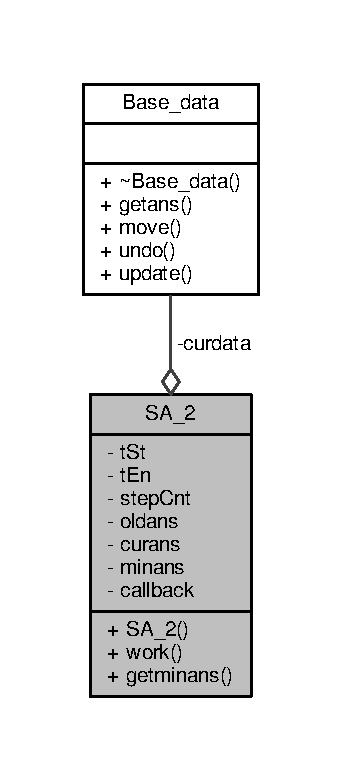
\includegraphics[width=164pt]{classSA__2__coll__graph}
\end{center}
\end{figure}
\subsection*{Public Types}
\begin{DoxyCompactItemize}
\item 
typedef void($\ast$ \hyperlink{classSA__2_a1c708dff32ff0526b5b5926e38e77dee}{callback\+\_\+t}) (int step, double temperature, double accept\+Wasted\+Rate, double min\+Wasted\+Rate)
\end{DoxyCompactItemize}
\subsection*{Public Member Functions}
\begin{DoxyCompactItemize}
\item 
\hyperlink{classSA__2_a14d69737deeebd1d413517bf013cd16f}{S\+A\+\_\+2} (double \+\_\+t\+St, double \+\_\+t\+En, int \+\_\+step\+Cnt, \hyperlink{classBase__data}{Base\+\_\+data} $\ast$, \hyperlink{classSA__2_a1c708dff32ff0526b5b5926e38e77dee}{callback\+\_\+t} \+\_\+callback=N\+U\+L\+L)
\item 
\hyperlink{classBase__data}{Base\+\_\+data} $\ast$ \hyperlink{classSA__2_a991bd4a7842fcaae442e0916445e45ae}{work} ()
\begin{DoxyCompactList}\small\item\em Main work loop. \end{DoxyCompactList}\item 
double \hyperlink{classSA__2_adbe6c7eb3f5c15b5ff72490de3be25c4}{getminans} ()
\end{DoxyCompactItemize}
\subsection*{Private Attributes}
\begin{DoxyCompactItemize}
\item 
double \hyperlink{classSA__2_a826b4a07815b519edd1821b07a0ed1f6}{t\+St}
\item 
double \hyperlink{classSA__2_a11eb83d386c783b62689b95a1d61f81b}{t\+En}
\item 
int \hyperlink{classSA__2_a9e6e985f337007134f5b82b18fc2a809}{step\+Cnt}
\item 
\hyperlink{classBase__data}{Base\+\_\+data} $\ast$ \hyperlink{classSA__2_ac333f4a2da95b01b271ba7ae422b6744}{curdata}
\item 
double \hyperlink{classSA__2_aea8cf021e1378fd37136fdff5c11b111}{oldans}
\item 
double \hyperlink{classSA__2_a40815916496d990e8bb324c52b33cc2f}{curans}
\item 
double \hyperlink{classSA__2_a93a9b121b39a9a88eac0ebdcc2d4c4e0}{minans}
\item 
\hyperlink{classSA__2_a1c708dff32ff0526b5b5926e38e77dee}{callback\+\_\+t} \hyperlink{classSA__2_a211a847edaaaf0e95f49b50d7355cc28}{callback}
\end{DoxyCompactItemize}


\subsection{Detailed Description}
Simulated Annealing. 

\subsection{Member Typedef Documentation}
\hypertarget{classSA__2_a1c708dff32ff0526b5b5926e38e77dee}{}\index{S\+A\+\_\+2@{S\+A\+\_\+2}!callback\+\_\+t@{callback\+\_\+t}}
\index{callback\+\_\+t@{callback\+\_\+t}!S\+A\+\_\+2@{S\+A\+\_\+2}}
\subsubsection[{callback\+\_\+t}]{\setlength{\rightskip}{0pt plus 5cm}typedef void($\ast$ S\+A\+\_\+2\+::callback\+\_\+t) (int step, double temperature, double accept\+Wasted\+Rate, double min\+Wasted\+Rate)}\label{classSA__2_a1c708dff32ff0526b5b5926e38e77dee}


\subsection{Constructor \& Destructor Documentation}
\hypertarget{classSA__2_a14d69737deeebd1d413517bf013cd16f}{}\index{S\+A\+\_\+2@{S\+A\+\_\+2}!S\+A\+\_\+2@{S\+A\+\_\+2}}
\index{S\+A\+\_\+2@{S\+A\+\_\+2}!S\+A\+\_\+2@{S\+A\+\_\+2}}
\subsubsection[{S\+A\+\_\+2}]{\setlength{\rightskip}{0pt plus 5cm}S\+A\+\_\+2\+::\+S\+A\+\_\+2 (
\begin{DoxyParamCaption}
\item[{double}]{\+\_\+t\+St, }
\item[{double}]{\+\_\+t\+En, }
\item[{int}]{\+\_\+step\+Cnt, }
\item[{{\bf Base\+\_\+data} $\ast$}]{\+\_\+data, }
\item[{{\bf callback\+\_\+t}}]{\+\_\+callback = {\ttfamily NULL}}
\end{DoxyParamCaption}
)}\label{classSA__2_a14d69737deeebd1d413517bf013cd16f}

\begin{DoxyParams}{Parameters}
{\em \+\_\+t\+En} & starting temperature \\
\hline
{\em \+\_\+step\+Cnt} & ending temperature (Temperature falls exponentially) \\
\hline
{\em \+\_\+data} & how many steps? \\
\hline
{\em \+\_\+callback} & The data stucture to storage the data callback to report parameters in each step \\
\hline
\end{DoxyParams}


\subsection{Member Function Documentation}
\hypertarget{classSA__2_adbe6c7eb3f5c15b5ff72490de3be25c4}{}\index{S\+A\+\_\+2@{S\+A\+\_\+2}!getminans@{getminans}}
\index{getminans@{getminans}!S\+A\+\_\+2@{S\+A\+\_\+2}}
\subsubsection[{getminans}]{\setlength{\rightskip}{0pt plus 5cm}double S\+A\+\_\+2\+::getminans (
\begin{DoxyParamCaption}
{}
\end{DoxyParamCaption}
)\hspace{0.3cm}{\ttfamily [inline]}}\label{classSA__2_adbe6c7eb3f5c15b5ff72490de3be25c4}
\hypertarget{classSA__2_a991bd4a7842fcaae442e0916445e45ae}{}\index{S\+A\+\_\+2@{S\+A\+\_\+2}!work@{work}}
\index{work@{work}!S\+A\+\_\+2@{S\+A\+\_\+2}}
\subsubsection[{work}]{\setlength{\rightskip}{0pt plus 5cm}{\bf Base\+\_\+data} $\ast$ S\+A\+\_\+2\+::work (
\begin{DoxyParamCaption}
{}
\end{DoxyParamCaption}
)}\label{classSA__2_a991bd4a7842fcaae442e0916445e45ae}


Main work loop. 

\begin{DoxyReturn}{Returns}
\+: final result 
\end{DoxyReturn}


\subsection{Member Data Documentation}
\hypertarget{classSA__2_a211a847edaaaf0e95f49b50d7355cc28}{}\index{S\+A\+\_\+2@{S\+A\+\_\+2}!callback@{callback}}
\index{callback@{callback}!S\+A\+\_\+2@{S\+A\+\_\+2}}
\subsubsection[{callback}]{\setlength{\rightskip}{0pt plus 5cm}{\bf callback\+\_\+t} S\+A\+\_\+2\+::callback\hspace{0.3cm}{\ttfamily [private]}}\label{classSA__2_a211a847edaaaf0e95f49b50d7355cc28}
\hypertarget{classSA__2_a40815916496d990e8bb324c52b33cc2f}{}\index{S\+A\+\_\+2@{S\+A\+\_\+2}!curans@{curans}}
\index{curans@{curans}!S\+A\+\_\+2@{S\+A\+\_\+2}}
\subsubsection[{curans}]{\setlength{\rightskip}{0pt plus 5cm}double S\+A\+\_\+2\+::curans\hspace{0.3cm}{\ttfamily [private]}}\label{classSA__2_a40815916496d990e8bb324c52b33cc2f}
\hypertarget{classSA__2_ac333f4a2da95b01b271ba7ae422b6744}{}\index{S\+A\+\_\+2@{S\+A\+\_\+2}!curdata@{curdata}}
\index{curdata@{curdata}!S\+A\+\_\+2@{S\+A\+\_\+2}}
\subsubsection[{curdata}]{\setlength{\rightskip}{0pt plus 5cm}{\bf Base\+\_\+data}$\ast$ S\+A\+\_\+2\+::curdata\hspace{0.3cm}{\ttfamily [private]}}\label{classSA__2_ac333f4a2da95b01b271ba7ae422b6744}
\hypertarget{classSA__2_a93a9b121b39a9a88eac0ebdcc2d4c4e0}{}\index{S\+A\+\_\+2@{S\+A\+\_\+2}!minans@{minans}}
\index{minans@{minans}!S\+A\+\_\+2@{S\+A\+\_\+2}}
\subsubsection[{minans}]{\setlength{\rightskip}{0pt plus 5cm}double S\+A\+\_\+2\+::minans\hspace{0.3cm}{\ttfamily [private]}}\label{classSA__2_a93a9b121b39a9a88eac0ebdcc2d4c4e0}
\hypertarget{classSA__2_aea8cf021e1378fd37136fdff5c11b111}{}\index{S\+A\+\_\+2@{S\+A\+\_\+2}!oldans@{oldans}}
\index{oldans@{oldans}!S\+A\+\_\+2@{S\+A\+\_\+2}}
\subsubsection[{oldans}]{\setlength{\rightskip}{0pt plus 5cm}double S\+A\+\_\+2\+::oldans\hspace{0.3cm}{\ttfamily [private]}}\label{classSA__2_aea8cf021e1378fd37136fdff5c11b111}
\hypertarget{classSA__2_a9e6e985f337007134f5b82b18fc2a809}{}\index{S\+A\+\_\+2@{S\+A\+\_\+2}!step\+Cnt@{step\+Cnt}}
\index{step\+Cnt@{step\+Cnt}!S\+A\+\_\+2@{S\+A\+\_\+2}}
\subsubsection[{step\+Cnt}]{\setlength{\rightskip}{0pt plus 5cm}int S\+A\+\_\+2\+::step\+Cnt\hspace{0.3cm}{\ttfamily [private]}}\label{classSA__2_a9e6e985f337007134f5b82b18fc2a809}
\hypertarget{classSA__2_a11eb83d386c783b62689b95a1d61f81b}{}\index{S\+A\+\_\+2@{S\+A\+\_\+2}!t\+En@{t\+En}}
\index{t\+En@{t\+En}!S\+A\+\_\+2@{S\+A\+\_\+2}}
\subsubsection[{t\+En}]{\setlength{\rightskip}{0pt plus 5cm}double S\+A\+\_\+2\+::t\+En\hspace{0.3cm}{\ttfamily [private]}}\label{classSA__2_a11eb83d386c783b62689b95a1d61f81b}
\hypertarget{classSA__2_a826b4a07815b519edd1821b07a0ed1f6}{}\index{S\+A\+\_\+2@{S\+A\+\_\+2}!t\+St@{t\+St}}
\index{t\+St@{t\+St}!S\+A\+\_\+2@{S\+A\+\_\+2}}
\subsubsection[{t\+St}]{\setlength{\rightskip}{0pt plus 5cm}double S\+A\+\_\+2\+::t\+St\hspace{0.3cm}{\ttfamily [private]}}\label{classSA__2_a826b4a07815b519edd1821b07a0ed1f6}


The documentation for this class was generated from the following files\+:\begin{DoxyCompactItemize}
\item 
\hyperlink{SA2_8h}{S\+A2.\+h}\item 
\hyperlink{SA2_8cpp}{S\+A2.\+cpp}\end{DoxyCompactItemize}

\hypertarget{structTTree_1_1subtree__t}{}\section{T\+Tree\+:\+:subtree\+\_\+t Struct Reference}
\label{structTTree_1_1subtree__t}\index{T\+Tree\+::subtree\+\_\+t@{T\+Tree\+::subtree\+\_\+t}}


Collaboration diagram for T\+Tree\+:\+:subtree\+\_\+t\+:
\nopagebreak
\begin{figure}[H]
\begin{center}
\leavevmode
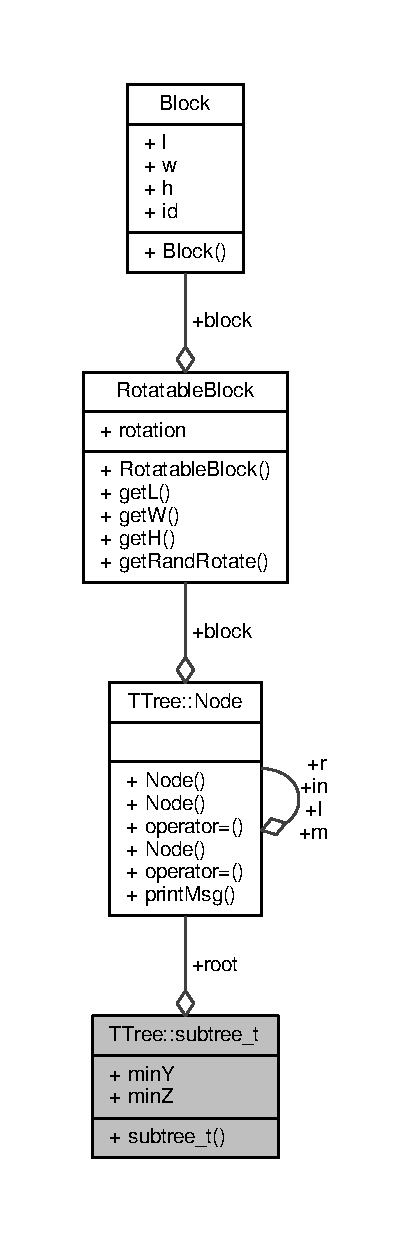
\includegraphics[height=550pt]{structTTree_1_1subtree__t__coll__graph}
\end{center}
\end{figure}
\subsection*{Public Member Functions}
\begin{DoxyCompactItemize}
\item 
\hyperlink{structTTree_1_1subtree__t_a39ba129f04bbc5c14f61e4055c575f34}{subtree\+\_\+t} (const \hyperlink{classTTree_1_1Node}{Node} $\ast$\+\_\+root, double \+\_\+min\+Y, double \+\_\+min\+Z)
\end{DoxyCompactItemize}
\subsection*{Public Attributes}
\begin{DoxyCompactItemize}
\item 
const \hyperlink{classTTree_1_1Node}{Node} $\ast$ \hyperlink{structTTree_1_1subtree__t_ab6ebbbb8aed78f23fbe1c5e59a290704}{root}
\item 
double \hyperlink{structTTree_1_1subtree__t_af9ebff6ea2db9188e99eb65fe7f3cc61}{min\+Y}
\item 
double \hyperlink{structTTree_1_1subtree__t_a3bcb871c4eeeaf275469ab86431381fa}{min\+Z}
\end{DoxyCompactItemize}


\subsection{Constructor \& Destructor Documentation}
\hypertarget{structTTree_1_1subtree__t_a39ba129f04bbc5c14f61e4055c575f34}{}\index{T\+Tree\+::subtree\+\_\+t@{T\+Tree\+::subtree\+\_\+t}!subtree\+\_\+t@{subtree\+\_\+t}}
\index{subtree\+\_\+t@{subtree\+\_\+t}!T\+Tree\+::subtree\+\_\+t@{T\+Tree\+::subtree\+\_\+t}}
\subsubsection[{subtree\+\_\+t}]{\setlength{\rightskip}{0pt plus 5cm}T\+Tree\+::subtree\+\_\+t\+::subtree\+\_\+t (
\begin{DoxyParamCaption}
\item[{const {\bf Node} $\ast$}]{\+\_\+root, }
\item[{double}]{\+\_\+min\+Y, }
\item[{double}]{\+\_\+min\+Z}
\end{DoxyParamCaption}
)\hspace{0.3cm}{\ttfamily [inline]}}\label{structTTree_1_1subtree__t_a39ba129f04bbc5c14f61e4055c575f34}


\subsection{Member Data Documentation}
\hypertarget{structTTree_1_1subtree__t_af9ebff6ea2db9188e99eb65fe7f3cc61}{}\index{T\+Tree\+::subtree\+\_\+t@{T\+Tree\+::subtree\+\_\+t}!min\+Y@{min\+Y}}
\index{min\+Y@{min\+Y}!T\+Tree\+::subtree\+\_\+t@{T\+Tree\+::subtree\+\_\+t}}
\subsubsection[{min\+Y}]{\setlength{\rightskip}{0pt plus 5cm}double T\+Tree\+::subtree\+\_\+t\+::min\+Y}\label{structTTree_1_1subtree__t_af9ebff6ea2db9188e99eb65fe7f3cc61}
\hypertarget{structTTree_1_1subtree__t_a3bcb871c4eeeaf275469ab86431381fa}{}\index{T\+Tree\+::subtree\+\_\+t@{T\+Tree\+::subtree\+\_\+t}!min\+Z@{min\+Z}}
\index{min\+Z@{min\+Z}!T\+Tree\+::subtree\+\_\+t@{T\+Tree\+::subtree\+\_\+t}}
\subsubsection[{min\+Z}]{\setlength{\rightskip}{0pt plus 5cm}double T\+Tree\+::subtree\+\_\+t\+::min\+Z}\label{structTTree_1_1subtree__t_a3bcb871c4eeeaf275469ab86431381fa}
\hypertarget{structTTree_1_1subtree__t_ab6ebbbb8aed78f23fbe1c5e59a290704}{}\index{T\+Tree\+::subtree\+\_\+t@{T\+Tree\+::subtree\+\_\+t}!root@{root}}
\index{root@{root}!T\+Tree\+::subtree\+\_\+t@{T\+Tree\+::subtree\+\_\+t}}
\subsubsection[{root}]{\setlength{\rightskip}{0pt plus 5cm}const {\bf Node}$\ast$ T\+Tree\+::subtree\+\_\+t\+::root}\label{structTTree_1_1subtree__t_ab6ebbbb8aed78f23fbe1c5e59a290704}


The documentation for this struct was generated from the following file\+:\begin{DoxyCompactItemize}
\item 
\hyperlink{TTree_8h}{T\+Tree.\+h}\end{DoxyCompactItemize}

\hypertarget{classTTree}{}\section{T\+Tree Class Reference}
\label{classTTree}\index{T\+Tree@{T\+Tree}}


{\ttfamily \#include $<$T\+Tree.\+h$>$}



Collaboration diagram for T\+Tree\+:
\nopagebreak
\begin{figure}[H]
\begin{center}
\leavevmode
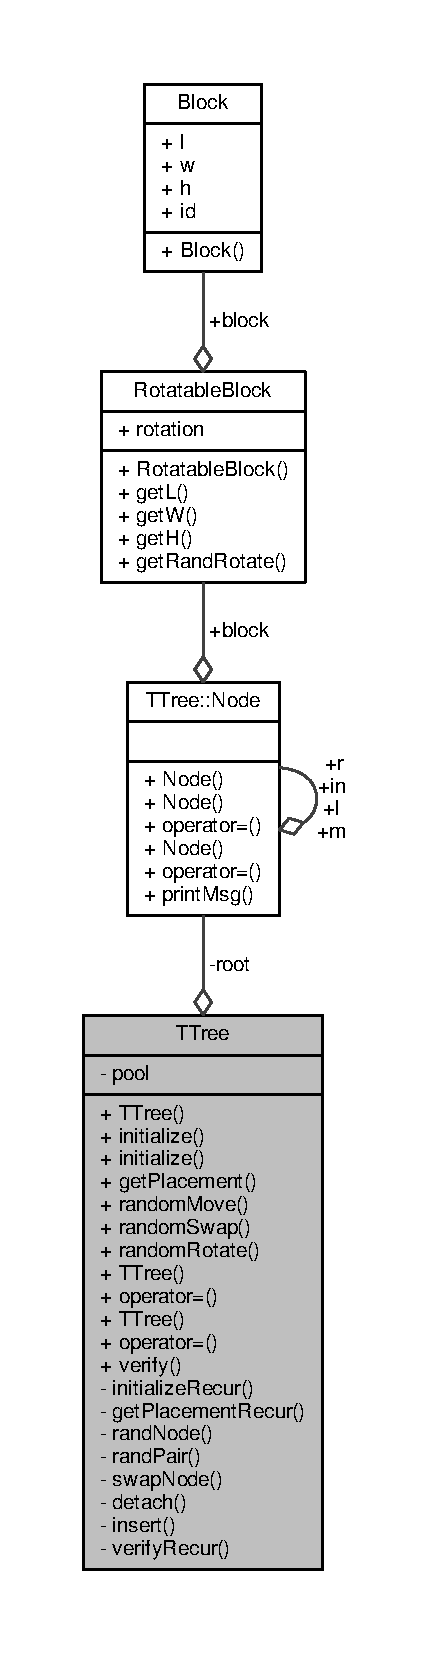
\includegraphics[height=550pt]{classTTree__coll__graph}
\end{center}
\end{figure}
\subsection*{Classes}
\begin{DoxyCompactItemize}
\item 
class \hyperlink{classTTree_1_1Node}{Node}
\begin{DoxyCompactList}\small\item\em Internal class. A node of T Tree. \end{DoxyCompactList}\item 
struct \hyperlink{structTTree_1_1subtree__t}{subtree\+\_\+t}
\end{DoxyCompactItemize}
\subsection*{Public Member Functions}
\begin{DoxyCompactItemize}
\item 
\hyperlink{classTTree_a86fa5aaf9e0e661ab3711fc70c99070e}{T\+Tree} ()
\item 
void \hyperlink{classTTree_a7be152bf003a3b7a41a0d2f2b8a60dcb}{initialize} (const std\+::vector$<$ \hyperlink{structBlock}{Block} $>$ \&blocks)
\begin{DoxyCompactList}\small\item\em Randomly initialize a tree with given blocks. \end{DoxyCompactList}\item 
void \hyperlink{classTTree_a39407b0d5bb0419d5930a264f909d240}{initialize} (std\+::vector$<$ const \hyperlink{structBlock}{Block} $\ast$ $>$ blocks)
\begin{DoxyCompactList}\small\item\em Randomly initialize a tree with given const blocks pointers. \end{DoxyCompactList}\item 
\hyperlink{classPlacement}{Placement} \hyperlink{classTTree_a7e34e70567be7961d4a5683010746aae}{get\+Placement} () const 
\begin{DoxyCompactList}\small\item\em Build a placement accroding to this tree. \end{DoxyCompactList}\item 
void \hyperlink{classTTree_a0b4e068faf77b43c5cb00a4e61a1c130}{random\+Move} ()
\begin{DoxyCompactList}\small\item\em Randomly move one node to another position. \end{DoxyCompactList}\item 
void \hyperlink{classTTree_aa5aab663511558247357bd9031f7f523}{random\+Swap} ()
\begin{DoxyCompactList}\small\item\em Randomly swap two nodes. \end{DoxyCompactList}\item 
void \hyperlink{classTTree_a72310af81f796797a623145656028bfc}{random\+Rotate} ()
\begin{DoxyCompactList}\small\item\em Randomly rotate one node\textquotesingle{}s block. \end{DoxyCompactList}\item 
void \hyperlink{classTTree_a14286d0dba4bda295b7a73ebefbf1bcf}{undo} ()
\begin{DoxyCompactList}\small\item\em Undo last operation. \end{DoxyCompactList}\item 
\hyperlink{classTTree_ad7fb8543e084eea4a24571f3cb979555}{T\+Tree} (const \hyperlink{classTTree}{T\+Tree} \&)=delete
\item 
\hyperlink{classTTree}{T\+Tree} \& \hyperlink{classTTree_a3c4da2361311ac5903822a2151865ae6}{operator=} (const \hyperlink{classTTree}{T\+Tree} \&)=delete
\item 
\hyperlink{classTTree_acfa1c1f035255298fd22be8810d5d672}{T\+Tree} (\hyperlink{classTTree}{T\+Tree} \&\&)=default
\item 
\hyperlink{classTTree}{T\+Tree} \& \hyperlink{classTTree_a8751a54d1c80d2f822d84a98e5c96293}{operator=} (\hyperlink{classTTree}{T\+Tree} \&\&)=default
\item 
void \hyperlink{classTTree_a561ca642fa6104a2275c30974b57e221}{verify} () const 
\begin{DoxyCompactList}\small\item\em Verify the some correctness of the tree. \end{DoxyCompactList}\end{DoxyCompactItemize}
\subsection*{Private Member Functions}
\begin{DoxyCompactItemize}
\item 
void \hyperlink{classTTree_aa4a9d2b247a7f9c33d1834fd23de7cca}{initialize\+Recur} (\hyperlink{classTTree_1_1Node}{Node} $\ast$\&p, size\+\_\+t id, const std\+::vector$<$ const \hyperlink{structBlock}{Block} $\ast$ $>$ \&blocks)
\begin{DoxyCompactList}\small\item\em Used by \hyperlink{classTTree_a7be152bf003a3b7a41a0d2f2b8a60dcb}{T\+Tree\+::initialize}. \end{DoxyCompactList}\item 
\hyperlink{structContourList_1_1Node}{Contour\+List\+::\+Node} $\ast$ \hyperlink{classTTree_a99a5f5452d13f1a3e4b74f8275224beb}{get\+Placement\+Recur} (const \hyperlink{classTTree_1_1Node}{Node} $\ast$p, \hyperlink{structContourList_1_1Node}{Contour\+List\+::\+Node} $\ast$q, double z, \hyperlink{classPlacement}{Placement} \&placement, std\+::list$<$ \hyperlink{structTTree_1_1subtree__t}{subtree\+\_\+t} $>$ \&subtrees) const 
\begin{DoxyCompactList}\small\item\em Used by \hyperlink{classTTree_a7e34e70567be7961d4a5683010746aae}{T\+Tree\+::get\+Placement}. \end{DoxyCompactList}\item 
\hyperlink{classTTree_1_1Node}{Node} $\ast$ \hyperlink{classTTree_acd9ed57c09bb59a5fcf618b8e215d584}{rand\+Node} ()
\begin{DoxyCompactList}\small\item\em Randomly choose a node. \end{DoxyCompactList}\item 
void \hyperlink{classTTree_aa756d0b900bc757b8095993d86fa5bd9}{rand\+Pair} (\hyperlink{classTTree_1_1Node}{Node} $\ast$\&p, \hyperlink{classTTree_1_1Node}{Node} $\ast$\&q)
\begin{DoxyCompactList}\small\item\em Randomly choose a pair of different nodes. \end{DoxyCompactList}\item 
void \hyperlink{classTTree_adbb05d027840467cdce8b9489bc49225}{swap\+Node} (\hyperlink{classTTree_1_1Node}{Node} $\ast$p, \hyperlink{classTTree_1_1Node}{Node} $\ast$q)
\begin{DoxyCompactList}\small\item\em Swap content of two node but not affecting the tree structure. \end{DoxyCompactList}\item 
\hyperlink{classTTree_1_1Node}{Node} $\ast$ \hyperlink{classTTree_ab9b74f48afd54c16fd1dc3b598019f7f}{detach} (\hyperlink{classTTree_1_1Node}{Node} $\ast$p)
\begin{DoxyCompactList}\small\item\em Detach a node from the tree. \end{DoxyCompactList}\item 
void \hyperlink{classTTree_a0bc18fd4039dc1ae0a53d2b68741a92b}{insert} (\hyperlink{classTTree_1_1Node}{Node} $\ast$parent, \hyperlink{classTTree_1_1Node}{Node} $\ast$child)
\begin{DoxyCompactList}\small\item\em Randomly insert node {\ttfamily child} as child of node {\ttfamily parent} \end{DoxyCompactList}\item 
void \hyperlink{classTTree_ab50938f36651a0cb2077ae84de2576a7}{verify\+Recur} (\hyperlink{classTTree_1_1Node}{Node} $\ast$const \&p, std\+::set$<$ const \hyperlink{structBlock}{Block} $\ast$ $>$ \&blocks) const 
\begin{DoxyCompactList}\small\item\em Used by Tree\+::verify. \end{DoxyCompactList}\end{DoxyCompactItemize}
\subsection*{Private Attributes}
\begin{DoxyCompactItemize}
\item 
\hyperlink{classTTree_1_1Node}{Node} $\ast$ \hyperlink{classTTree_a76972bd24a6d2f940fe1645d008a4a04}{root}
\item 
std\+::vector$<$ \hyperlink{classTTree_1_1Node}{Node} $>$ \hyperlink{classTTree_a58f7a793347834e9caee3d87c7202966}{pool}
\begin{DoxyCompactList}\small\item\em \hyperlink{classTTree_1_1Node}{Node} pool. This helps map an id to a node. \end{DoxyCompactList}\item 
std\+::vector$<$ \hyperlink{classTTree_1_1Node}{Node} $\ast$ $>$ \hyperlink{classTTree_a384e0ade54dfcb4688d646e3674e964a}{undo\+List}
\begin{DoxyCompactList}\small\item\em Nodes that need to undo. \end{DoxyCompactList}\end{DoxyCompactItemize}


\subsection{Constructor \& Destructor Documentation}
\hypertarget{classTTree_a86fa5aaf9e0e661ab3711fc70c99070e}{}\index{T\+Tree@{T\+Tree}!T\+Tree@{T\+Tree}}
\index{T\+Tree@{T\+Tree}!T\+Tree@{T\+Tree}}
\subsubsection[{T\+Tree}]{\setlength{\rightskip}{0pt plus 5cm}T\+Tree\+::\+T\+Tree (
\begin{DoxyParamCaption}
{}
\end{DoxyParamCaption}
)\hspace{0.3cm}{\ttfamily [inline]}}\label{classTTree_a86fa5aaf9e0e661ab3711fc70c99070e}
\hypertarget{classTTree_ad7fb8543e084eea4a24571f3cb979555}{}\index{T\+Tree@{T\+Tree}!T\+Tree@{T\+Tree}}
\index{T\+Tree@{T\+Tree}!T\+Tree@{T\+Tree}}
\subsubsection[{T\+Tree}]{\setlength{\rightskip}{0pt plus 5cm}T\+Tree\+::\+T\+Tree (
\begin{DoxyParamCaption}
\item[{const {\bf T\+Tree} \&}]{}
\end{DoxyParamCaption}
)\hspace{0.3cm}{\ttfamily [delete]}}\label{classTTree_ad7fb8543e084eea4a24571f3cb979555}
\hypertarget{classTTree_acfa1c1f035255298fd22be8810d5d672}{}\index{T\+Tree@{T\+Tree}!T\+Tree@{T\+Tree}}
\index{T\+Tree@{T\+Tree}!T\+Tree@{T\+Tree}}
\subsubsection[{T\+Tree}]{\setlength{\rightskip}{0pt plus 5cm}T\+Tree\+::\+T\+Tree (
\begin{DoxyParamCaption}
\item[{{\bf T\+Tree} \&\&}]{}
\end{DoxyParamCaption}
)\hspace{0.3cm}{\ttfamily [default]}}\label{classTTree_acfa1c1f035255298fd22be8810d5d672}


\subsection{Member Function Documentation}
\hypertarget{classTTree_ab9b74f48afd54c16fd1dc3b598019f7f}{}\index{T\+Tree@{T\+Tree}!detach@{detach}}
\index{detach@{detach}!T\+Tree@{T\+Tree}}
\subsubsection[{detach}]{\setlength{\rightskip}{0pt plus 5cm}{\bf T\+Tree\+::\+Node} $\ast$ T\+Tree\+::detach (
\begin{DoxyParamCaption}
\item[{{\bf T\+Tree\+::\+Node} $\ast$}]{p}
\end{DoxyParamCaption}
)\hspace{0.3cm}{\ttfamily [private]}}\label{classTTree_ab9b74f48afd54c16fd1dc3b598019f7f}


Detach a node from the tree. 

This is a random procedure. \begin{DoxyReturn}{Returns}
The node 
\end{DoxyReturn}
\hypertarget{classTTree_a7e34e70567be7961d4a5683010746aae}{}\index{T\+Tree@{T\+Tree}!get\+Placement@{get\+Placement}}
\index{get\+Placement@{get\+Placement}!T\+Tree@{T\+Tree}}
\subsubsection[{get\+Placement}]{\setlength{\rightskip}{0pt plus 5cm}{\bf Placement} T\+Tree\+::get\+Placement (
\begin{DoxyParamCaption}
{}
\end{DoxyParamCaption}
) const}\label{classTTree_a7e34e70567be7961d4a5683010746aae}


Build a placement accroding to this tree. 

O(n). n is the number of the nodes. \hypertarget{classTTree_a99a5f5452d13f1a3e4b74f8275224beb}{}\index{T\+Tree@{T\+Tree}!get\+Placement\+Recur@{get\+Placement\+Recur}}
\index{get\+Placement\+Recur@{get\+Placement\+Recur}!T\+Tree@{T\+Tree}}
\subsubsection[{get\+Placement\+Recur}]{\setlength{\rightskip}{0pt plus 5cm}{\bf Contour\+List\+::\+Node} $\ast$ T\+Tree\+::get\+Placement\+Recur (
\begin{DoxyParamCaption}
\item[{const {\bf Node} $\ast$}]{p, }
\item[{{\bf Contour\+List\+::\+Node} $\ast$}]{q, }
\item[{double}]{z, }
\item[{{\bf Placement} \&}]{placement, }
\item[{std\+::list$<$ {\bf subtree\+\_\+t} $>$ \&}]{subtrees}
\end{DoxyParamCaption}
) const\hspace{0.3cm}{\ttfamily [private]}}\label{classTTree_a99a5f5452d13f1a3e4b74f8275224beb}


Used by \hyperlink{classTTree_a7e34e70567be7961d4a5683010746aae}{T\+Tree\+::get\+Placement}. 

\begin{DoxyReturn}{Returns}
The node replaced q 
\end{DoxyReturn}
\hypertarget{classTTree_a7be152bf003a3b7a41a0d2f2b8a60dcb}{}\index{T\+Tree@{T\+Tree}!initialize@{initialize}}
\index{initialize@{initialize}!T\+Tree@{T\+Tree}}
\subsubsection[{initialize}]{\setlength{\rightskip}{0pt plus 5cm}void T\+Tree\+::initialize (
\begin{DoxyParamCaption}
\item[{const std\+::vector$<$ {\bf Block} $>$ \&}]{blocks}
\end{DoxyParamCaption}
)}\label{classTTree_a7be152bf003a3b7a41a0d2f2b8a60dcb}


Randomly initialize a tree with given blocks. 

\hypertarget{classTTree_a39407b0d5bb0419d5930a264f909d240}{}\index{T\+Tree@{T\+Tree}!initialize@{initialize}}
\index{initialize@{initialize}!T\+Tree@{T\+Tree}}
\subsubsection[{initialize}]{\setlength{\rightskip}{0pt plus 5cm}void T\+Tree\+::initialize (
\begin{DoxyParamCaption}
\item[{std\+::vector$<$ const {\bf Block} $\ast$ $>$}]{blocks}
\end{DoxyParamCaption}
)}\label{classTTree_a39407b0d5bb0419d5930a264f909d240}


Randomly initialize a tree with given const blocks pointers. 


\begin{DoxyParams}{Parameters}
{\em blocks} & The given blocks. Shouldn\textquotesingle{}t be const \& \\
\hline
\end{DoxyParams}
\hypertarget{classTTree_aa4a9d2b247a7f9c33d1834fd23de7cca}{}\index{T\+Tree@{T\+Tree}!initialize\+Recur@{initialize\+Recur}}
\index{initialize\+Recur@{initialize\+Recur}!T\+Tree@{T\+Tree}}
\subsubsection[{initialize\+Recur}]{\setlength{\rightskip}{0pt plus 5cm}void T\+Tree\+::initialize\+Recur (
\begin{DoxyParamCaption}
\item[{{\bf Node} $\ast$\&}]{p, }
\item[{size\+\_\+t}]{id, }
\item[{const std\+::vector$<$ const {\bf Block} $\ast$ $>$ \&}]{blocks}
\end{DoxyParamCaption}
)\hspace{0.3cm}{\ttfamily [private]}}\label{classTTree_aa4a9d2b247a7f9c33d1834fd23de7cca}


Used by \hyperlink{classTTree_a7be152bf003a3b7a41a0d2f2b8a60dcb}{T\+Tree\+::initialize}. 

\hypertarget{classTTree_a0bc18fd4039dc1ae0a53d2b68741a92b}{}\index{T\+Tree@{T\+Tree}!insert@{insert}}
\index{insert@{insert}!T\+Tree@{T\+Tree}}
\subsubsection[{insert}]{\setlength{\rightskip}{0pt plus 5cm}void T\+Tree\+::insert (
\begin{DoxyParamCaption}
\item[{{\bf Node} $\ast$}]{parent, }
\item[{{\bf Node} $\ast$}]{child}
\end{DoxyParamCaption}
)\hspace{0.3cm}{\ttfamily [private]}}\label{classTTree_a0bc18fd4039dc1ae0a53d2b68741a92b}


Randomly insert node {\ttfamily child} as child of node {\ttfamily parent} 

\hypertarget{classTTree_a3c4da2361311ac5903822a2151865ae6}{}\index{T\+Tree@{T\+Tree}!operator=@{operator=}}
\index{operator=@{operator=}!T\+Tree@{T\+Tree}}
\subsubsection[{operator=}]{\setlength{\rightskip}{0pt plus 5cm}{\bf T\+Tree}\& T\+Tree\+::operator= (
\begin{DoxyParamCaption}
\item[{const {\bf T\+Tree} \&}]{}
\end{DoxyParamCaption}
)\hspace{0.3cm}{\ttfamily [delete]}}\label{classTTree_a3c4da2361311ac5903822a2151865ae6}
\hypertarget{classTTree_a8751a54d1c80d2f822d84a98e5c96293}{}\index{T\+Tree@{T\+Tree}!operator=@{operator=}}
\index{operator=@{operator=}!T\+Tree@{T\+Tree}}
\subsubsection[{operator=}]{\setlength{\rightskip}{0pt plus 5cm}{\bf T\+Tree}\& T\+Tree\+::operator= (
\begin{DoxyParamCaption}
\item[{{\bf T\+Tree} \&\&}]{}
\end{DoxyParamCaption}
)\hspace{0.3cm}{\ttfamily [default]}}\label{classTTree_a8751a54d1c80d2f822d84a98e5c96293}
\hypertarget{classTTree_acd9ed57c09bb59a5fcf618b8e215d584}{}\index{T\+Tree@{T\+Tree}!rand\+Node@{rand\+Node}}
\index{rand\+Node@{rand\+Node}!T\+Tree@{T\+Tree}}
\subsubsection[{rand\+Node}]{\setlength{\rightskip}{0pt plus 5cm}{\bf T\+Tree\+::\+Node} $\ast$ T\+Tree\+::rand\+Node (
\begin{DoxyParamCaption}
{}
\end{DoxyParamCaption}
)\hspace{0.3cm}{\ttfamily [inline]}, {\ttfamily [private]}}\label{classTTree_acd9ed57c09bb59a5fcf618b8e215d584}


Randomly choose a node. 

\hypertarget{classTTree_a0b4e068faf77b43c5cb00a4e61a1c130}{}\index{T\+Tree@{T\+Tree}!random\+Move@{random\+Move}}
\index{random\+Move@{random\+Move}!T\+Tree@{T\+Tree}}
\subsubsection[{random\+Move}]{\setlength{\rightskip}{0pt plus 5cm}void T\+Tree\+::random\+Move (
\begin{DoxyParamCaption}
{}
\end{DoxyParamCaption}
)}\label{classTTree_a0b4e068faf77b43c5cb00a4e61a1c130}


Randomly move one node to another position. 

Requires at least 3 nodes in the tree. O(h). h is the height of the tree. \hypertarget{classTTree_a72310af81f796797a623145656028bfc}{}\index{T\+Tree@{T\+Tree}!random\+Rotate@{random\+Rotate}}
\index{random\+Rotate@{random\+Rotate}!T\+Tree@{T\+Tree}}
\subsubsection[{random\+Rotate}]{\setlength{\rightskip}{0pt plus 5cm}void T\+Tree\+::random\+Rotate (
\begin{DoxyParamCaption}
{}
\end{DoxyParamCaption}
)}\label{classTTree_a72310af81f796797a623145656028bfc}


Randomly rotate one node\textquotesingle{}s block. 

O(1). \hypertarget{classTTree_aa5aab663511558247357bd9031f7f523}{}\index{T\+Tree@{T\+Tree}!random\+Swap@{random\+Swap}}
\index{random\+Swap@{random\+Swap}!T\+Tree@{T\+Tree}}
\subsubsection[{random\+Swap}]{\setlength{\rightskip}{0pt plus 5cm}void T\+Tree\+::random\+Swap (
\begin{DoxyParamCaption}
{}
\end{DoxyParamCaption}
)}\label{classTTree_aa5aab663511558247357bd9031f7f523}


Randomly swap two nodes. 

Requires at least 2 nodes in the tree. O(1). \hypertarget{classTTree_aa756d0b900bc757b8095993d86fa5bd9}{}\index{T\+Tree@{T\+Tree}!rand\+Pair@{rand\+Pair}}
\index{rand\+Pair@{rand\+Pair}!T\+Tree@{T\+Tree}}
\subsubsection[{rand\+Pair}]{\setlength{\rightskip}{0pt plus 5cm}void T\+Tree\+::rand\+Pair (
\begin{DoxyParamCaption}
\item[{{\bf Node} $\ast$\&}]{p, }
\item[{{\bf Node} $\ast$\&}]{q}
\end{DoxyParamCaption}
)\hspace{0.3cm}{\ttfamily [inline]}, {\ttfamily [private]}}\label{classTTree_aa756d0b900bc757b8095993d86fa5bd9}


Randomly choose a pair of different nodes. 

\hypertarget{classTTree_adbb05d027840467cdce8b9489bc49225}{}\index{T\+Tree@{T\+Tree}!swap\+Node@{swap\+Node}}
\index{swap\+Node@{swap\+Node}!T\+Tree@{T\+Tree}}
\subsubsection[{swap\+Node}]{\setlength{\rightskip}{0pt plus 5cm}void T\+Tree\+::swap\+Node (
\begin{DoxyParamCaption}
\item[{{\bf T\+Tree\+::\+Node} $\ast$}]{p, }
\item[{{\bf T\+Tree\+::\+Node} $\ast$}]{q}
\end{DoxyParamCaption}
)\hspace{0.3cm}{\ttfamily [private]}}\label{classTTree_adbb05d027840467cdce8b9489bc49225}


Swap content of two node but not affecting the tree structure. 

\hypertarget{classTTree_a14286d0dba4bda295b7a73ebefbf1bcf}{}\index{T\+Tree@{T\+Tree}!undo@{undo}}
\index{undo@{undo}!T\+Tree@{T\+Tree}}
\subsubsection[{undo}]{\setlength{\rightskip}{0pt plus 5cm}void T\+Tree\+::undo (
\begin{DoxyParamCaption}
{}
\end{DoxyParamCaption}
)}\label{classTTree_a14286d0dba4bda295b7a73ebefbf1bcf}


Undo last operation. 

\hypertarget{classTTree_a561ca642fa6104a2275c30974b57e221}{}\index{T\+Tree@{T\+Tree}!verify@{verify}}
\index{verify@{verify}!T\+Tree@{T\+Tree}}
\subsubsection[{verify}]{\setlength{\rightskip}{0pt plus 5cm}void T\+Tree\+::verify (
\begin{DoxyParamCaption}
{}
\end{DoxyParamCaption}
) const}\label{classTTree_a561ca642fa6104a2275c30974b57e221}


Verify the some correctness of the tree. 

Uses assert. \hypertarget{classTTree_ab50938f36651a0cb2077ae84de2576a7}{}\index{T\+Tree@{T\+Tree}!verify\+Recur@{verify\+Recur}}
\index{verify\+Recur@{verify\+Recur}!T\+Tree@{T\+Tree}}
\subsubsection[{verify\+Recur}]{\setlength{\rightskip}{0pt plus 5cm}void T\+Tree\+::verify\+Recur (
\begin{DoxyParamCaption}
\item[{{\bf Node} $\ast$const \&}]{p, }
\item[{std\+::set$<$ const {\bf Block} $\ast$ $>$ \&}]{blocks}
\end{DoxyParamCaption}
) const\hspace{0.3cm}{\ttfamily [private]}}\label{classTTree_ab50938f36651a0cb2077ae84de2576a7}


Used by Tree\+::verify. 


\begin{DoxyParams}{Parameters}
{\em p} & Should be $\ast$ const \&, instead of const $\ast$ const \&. Type conversion will change the address \\
\hline
\end{DoxyParams}


\subsection{Member Data Documentation}
\hypertarget{classTTree_a58f7a793347834e9caee3d87c7202966}{}\index{T\+Tree@{T\+Tree}!pool@{pool}}
\index{pool@{pool}!T\+Tree@{T\+Tree}}
\subsubsection[{pool}]{\setlength{\rightskip}{0pt plus 5cm}std\+::vector$<${\bf Node}$>$ T\+Tree\+::pool\hspace{0.3cm}{\ttfamily [private]}}\label{classTTree_a58f7a793347834e9caee3d87c7202966}


\hyperlink{classTTree_1_1Node}{Node} pool. This helps map an id to a node. 

\hypertarget{classTTree_a76972bd24a6d2f940fe1645d008a4a04}{}\index{T\+Tree@{T\+Tree}!root@{root}}
\index{root@{root}!T\+Tree@{T\+Tree}}
\subsubsection[{root}]{\setlength{\rightskip}{0pt plus 5cm}{\bf Node}$\ast$ T\+Tree\+::root\hspace{0.3cm}{\ttfamily [private]}}\label{classTTree_a76972bd24a6d2f940fe1645d008a4a04}
\hypertarget{classTTree_a384e0ade54dfcb4688d646e3674e964a}{}\index{T\+Tree@{T\+Tree}!undo\+List@{undo\+List}}
\index{undo\+List@{undo\+List}!T\+Tree@{T\+Tree}}
\subsubsection[{undo\+List}]{\setlength{\rightskip}{0pt plus 5cm}std\+::vector$<${\bf Node}$\ast$$>$ T\+Tree\+::undo\+List\hspace{0.3cm}{\ttfamily [private]}}\label{classTTree_a384e0ade54dfcb4688d646e3674e964a}


Nodes that need to undo. 



The documentation for this class was generated from the following files\+:\begin{DoxyCompactItemize}
\item 
\hyperlink{TTree_8h}{T\+Tree.\+h}\item 
\hyperlink{TTree_8cpp}{T\+Tree.\+cpp}\end{DoxyCompactItemize}

\hypertarget{classTTree__data}{}\section{T\+Tree\+\_\+data Class Reference}
\label{classTTree__data}\index{T\+Tree\+\_\+data@{T\+Tree\+\_\+data}}


{\ttfamily \#include $<$T\+Treedata.\+h$>$}



Inheritance diagram for T\+Tree\+\_\+data\+:
\nopagebreak
\begin{figure}[H]
\begin{center}
\leavevmode
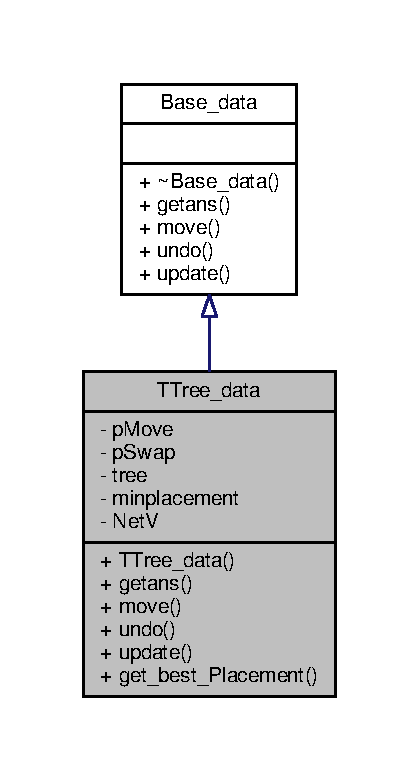
\includegraphics[width=201pt]{classTTree__data__inherit__graph}
\end{center}
\end{figure}


Collaboration diagram for T\+Tree\+\_\+data\+:
\nopagebreak
\begin{figure}[H]
\begin{center}
\leavevmode
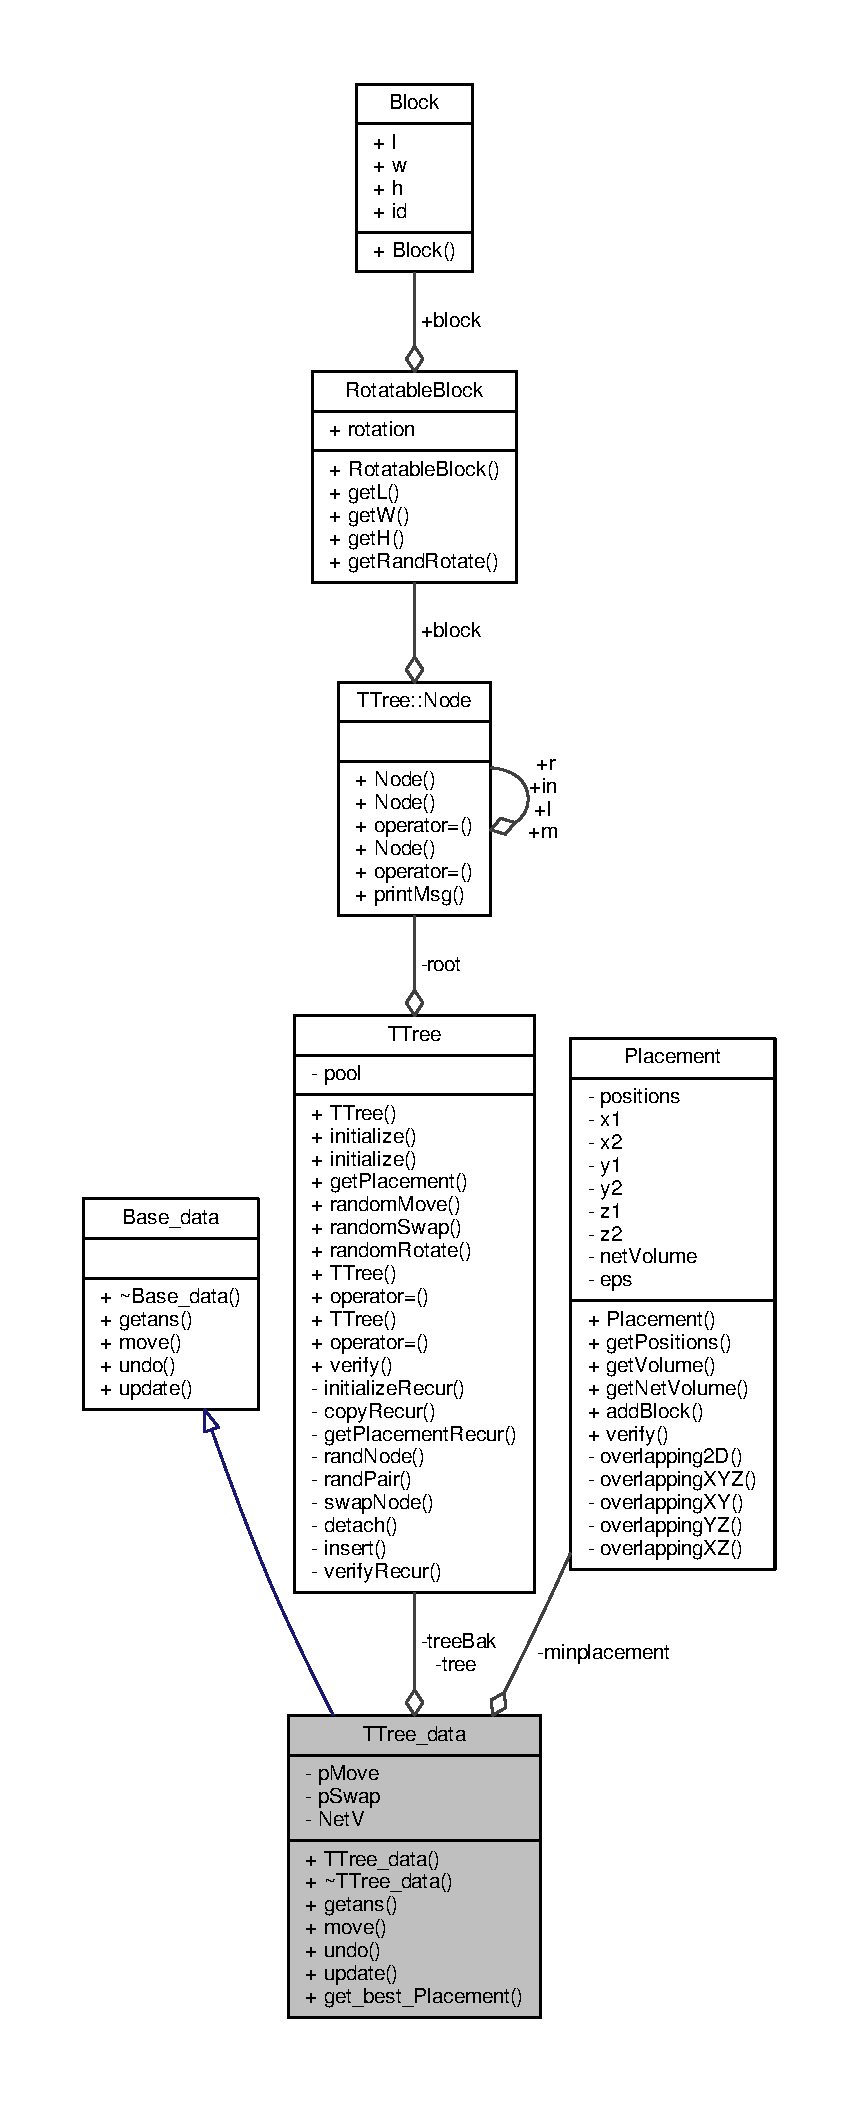
\includegraphics[height=550pt]{classTTree__data__coll__graph}
\end{center}
\end{figure}
\subsection*{Public Member Functions}
\begin{DoxyCompactItemize}
\item 
\hyperlink{classTTree__data_a5c15fc4f6ad8453e6de07e3defd1faeb}{T\+Tree\+\_\+data} (double \+\_\+p\+Move, double \+\_\+p\+Swap, \hyperlink{classTTree}{T\+Tree} $\ast$\+\_\+tree)
\item 
double \hyperlink{classTTree__data_a2524c0f18f01378fc80fd558e3b7cebb}{getans} ()
\item 
void \hyperlink{classTTree__data_a16a5d735999764d45d38d2327955696e}{move} ()
\item 
void \hyperlink{classTTree__data_ac2f447392cb0cf81db44d4f85d4bfd8a}{undo} ()
\item 
void \hyperlink{classTTree__data_a828b99a40bab8933fd3c648ee4f10d85}{update} ()
\item 
\hyperlink{classPlacement}{Placement} \hyperlink{classTTree__data_a4043bb9cd9f3d3b2509653d567c11fa8}{get\+\_\+best\+\_\+\+Placement} ()
\end{DoxyCompactItemize}
\subsection*{Private Attributes}
\begin{DoxyCompactItemize}
\item 
double \hyperlink{classTTree__data_a45c965402cccc4fd9a4cfcffd3fb991f}{p\+Move}
\item 
double \hyperlink{classTTree__data_a14ad1213b452c13d7385fbf6f74e1fcf}{p\+Swap}
\item 
\hyperlink{classTTree}{T\+Tree} $\ast$ \hyperlink{classTTree__data_adb6a018eb7424a0205ff478287dffab5}{tree}
\item 
\hyperlink{classPlacement}{Placement} \hyperlink{classTTree__data_af901c9da93c6d1558565c919019e2aa8}{minplacement}
\item 
double \hyperlink{classTTree__data_ab63ddf6e7ecf680762cc3af591986d73}{Net\+V}
\end{DoxyCompactItemize}


\subsection{Constructor \& Destructor Documentation}
\hypertarget{classTTree__data_a5c15fc4f6ad8453e6de07e3defd1faeb}{}\index{T\+Tree\+\_\+data@{T\+Tree\+\_\+data}!T\+Tree\+\_\+data@{T\+Tree\+\_\+data}}
\index{T\+Tree\+\_\+data@{T\+Tree\+\_\+data}!T\+Tree\+\_\+data@{T\+Tree\+\_\+data}}
\subsubsection[{T\+Tree\+\_\+data}]{\setlength{\rightskip}{0pt plus 5cm}T\+Tree\+\_\+data\+::\+T\+Tree\+\_\+data (
\begin{DoxyParamCaption}
\item[{double}]{\+\_\+p\+Move, }
\item[{double}]{\+\_\+p\+Swap, }
\item[{{\bf T\+Tree} $\ast$}]{\+\_\+tree}
\end{DoxyParamCaption}
)}\label{classTTree__data_a5c15fc4f6ad8453e6de07e3defd1faeb}


\subsection{Member Function Documentation}
\hypertarget{classTTree__data_a4043bb9cd9f3d3b2509653d567c11fa8}{}\index{T\+Tree\+\_\+data@{T\+Tree\+\_\+data}!get\+\_\+best\+\_\+\+Placement@{get\+\_\+best\+\_\+\+Placement}}
\index{get\+\_\+best\+\_\+\+Placement@{get\+\_\+best\+\_\+\+Placement}!T\+Tree\+\_\+data@{T\+Tree\+\_\+data}}
\subsubsection[{get\+\_\+best\+\_\+\+Placement}]{\setlength{\rightskip}{0pt plus 5cm}{\bf Placement} T\+Tree\+\_\+data\+::get\+\_\+best\+\_\+\+Placement (
\begin{DoxyParamCaption}
{}
\end{DoxyParamCaption}
)\hspace{0.3cm}{\ttfamily [inline]}}\label{classTTree__data_a4043bb9cd9f3d3b2509653d567c11fa8}
\hypertarget{classTTree__data_a2524c0f18f01378fc80fd558e3b7cebb}{}\index{T\+Tree\+\_\+data@{T\+Tree\+\_\+data}!getans@{getans}}
\index{getans@{getans}!T\+Tree\+\_\+data@{T\+Tree\+\_\+data}}
\subsubsection[{getans}]{\setlength{\rightskip}{0pt plus 5cm}double T\+Tree\+\_\+data\+::getans (
\begin{DoxyParamCaption}
{}
\end{DoxyParamCaption}
)\hspace{0.3cm}{\ttfamily [inline]}, {\ttfamily [virtual]}}\label{classTTree__data_a2524c0f18f01378fc80fd558e3b7cebb}


Implements \hyperlink{classBase__data_a30c68b7fadf62354a5291e63c826a6b1}{Base\+\_\+data}.

\hypertarget{classTTree__data_a16a5d735999764d45d38d2327955696e}{}\index{T\+Tree\+\_\+data@{T\+Tree\+\_\+data}!move@{move}}
\index{move@{move}!T\+Tree\+\_\+data@{T\+Tree\+\_\+data}}
\subsubsection[{move}]{\setlength{\rightskip}{0pt plus 5cm}void T\+Tree\+\_\+data\+::move (
\begin{DoxyParamCaption}
{}
\end{DoxyParamCaption}
)\hspace{0.3cm}{\ttfamily [virtual]}}\label{classTTree__data_a16a5d735999764d45d38d2327955696e}


Implements \hyperlink{classBase__data_ae471e1151062f17bf299dc72dcfdd73a}{Base\+\_\+data}.

\hypertarget{classTTree__data_ac2f447392cb0cf81db44d4f85d4bfd8a}{}\index{T\+Tree\+\_\+data@{T\+Tree\+\_\+data}!undo@{undo}}
\index{undo@{undo}!T\+Tree\+\_\+data@{T\+Tree\+\_\+data}}
\subsubsection[{undo}]{\setlength{\rightskip}{0pt plus 5cm}void T\+Tree\+\_\+data\+::undo (
\begin{DoxyParamCaption}
{}
\end{DoxyParamCaption}
)\hspace{0.3cm}{\ttfamily [inline]}, {\ttfamily [virtual]}}\label{classTTree__data_ac2f447392cb0cf81db44d4f85d4bfd8a}


Implements \hyperlink{classBase__data_ab7486d1e6e1c199b637cb1473daf9a14}{Base\+\_\+data}.

\hypertarget{classTTree__data_a828b99a40bab8933fd3c648ee4f10d85}{}\index{T\+Tree\+\_\+data@{T\+Tree\+\_\+data}!update@{update}}
\index{update@{update}!T\+Tree\+\_\+data@{T\+Tree\+\_\+data}}
\subsubsection[{update}]{\setlength{\rightskip}{0pt plus 5cm}void T\+Tree\+\_\+data\+::update (
\begin{DoxyParamCaption}
{}
\end{DoxyParamCaption}
)\hspace{0.3cm}{\ttfamily [inline]}, {\ttfamily [virtual]}}\label{classTTree__data_a828b99a40bab8933fd3c648ee4f10d85}


Implements \hyperlink{classBase__data_a8545b22fc79ece9d036731ecb3db7b5d}{Base\+\_\+data}.



\subsection{Member Data Documentation}
\hypertarget{classTTree__data_af901c9da93c6d1558565c919019e2aa8}{}\index{T\+Tree\+\_\+data@{T\+Tree\+\_\+data}!minplacement@{minplacement}}
\index{minplacement@{minplacement}!T\+Tree\+\_\+data@{T\+Tree\+\_\+data}}
\subsubsection[{minplacement}]{\setlength{\rightskip}{0pt plus 5cm}{\bf Placement} T\+Tree\+\_\+data\+::minplacement\hspace{0.3cm}{\ttfamily [private]}}\label{classTTree__data_af901c9da93c6d1558565c919019e2aa8}
\hypertarget{classTTree__data_ab63ddf6e7ecf680762cc3af591986d73}{}\index{T\+Tree\+\_\+data@{T\+Tree\+\_\+data}!Net\+V@{Net\+V}}
\index{Net\+V@{Net\+V}!T\+Tree\+\_\+data@{T\+Tree\+\_\+data}}
\subsubsection[{Net\+V}]{\setlength{\rightskip}{0pt plus 5cm}double T\+Tree\+\_\+data\+::\+Net\+V\hspace{0.3cm}{\ttfamily [private]}}\label{classTTree__data_ab63ddf6e7ecf680762cc3af591986d73}
\hypertarget{classTTree__data_a45c965402cccc4fd9a4cfcffd3fb991f}{}\index{T\+Tree\+\_\+data@{T\+Tree\+\_\+data}!p\+Move@{p\+Move}}
\index{p\+Move@{p\+Move}!T\+Tree\+\_\+data@{T\+Tree\+\_\+data}}
\subsubsection[{p\+Move}]{\setlength{\rightskip}{0pt plus 5cm}double T\+Tree\+\_\+data\+::p\+Move\hspace{0.3cm}{\ttfamily [private]}}\label{classTTree__data_a45c965402cccc4fd9a4cfcffd3fb991f}
\hypertarget{classTTree__data_a14ad1213b452c13d7385fbf6f74e1fcf}{}\index{T\+Tree\+\_\+data@{T\+Tree\+\_\+data}!p\+Swap@{p\+Swap}}
\index{p\+Swap@{p\+Swap}!T\+Tree\+\_\+data@{T\+Tree\+\_\+data}}
\subsubsection[{p\+Swap}]{\setlength{\rightskip}{0pt plus 5cm}double T\+Tree\+\_\+data\+::p\+Swap\hspace{0.3cm}{\ttfamily [private]}}\label{classTTree__data_a14ad1213b452c13d7385fbf6f74e1fcf}
\hypertarget{classTTree__data_adb6a018eb7424a0205ff478287dffab5}{}\index{T\+Tree\+\_\+data@{T\+Tree\+\_\+data}!tree@{tree}}
\index{tree@{tree}!T\+Tree\+\_\+data@{T\+Tree\+\_\+data}}
\subsubsection[{tree}]{\setlength{\rightskip}{0pt plus 5cm}{\bf T\+Tree}$\ast$ T\+Tree\+\_\+data\+::tree\hspace{0.3cm}{\ttfamily [private]}}\label{classTTree__data_adb6a018eb7424a0205ff478287dffab5}


The documentation for this class was generated from the following files\+:\begin{DoxyCompactItemize}
\item 
\hyperlink{TTreedata_8h}{T\+Treedata.\+h}\item 
\hyperlink{TTreedata_8cpp}{T\+Treedata.\+cpp}\end{DoxyCompactItemize}

\chapter{File Documentation}
\hypertarget{Basedata_8h}{}\section{Basedata.\+h File Reference}
\label{Basedata_8h}\index{Basedata.\+h@{Basedata.\+h}}
This graph shows which files directly or indirectly include this file\+:
\nopagebreak
\begin{figure}[H]
\begin{center}
\leavevmode
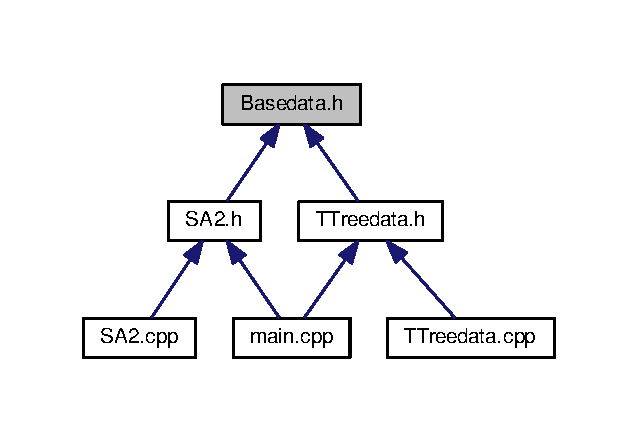
\includegraphics[width=306pt]{Basedata_8h__dep__incl}
\end{center}
\end{figure}
\subsection*{Classes}
\begin{DoxyCompactItemize}
\item 
class \hyperlink{classBase__data}{Base\+\_\+data}
\begin{DoxyCompactList}\small\item\em Data interface used by S\+A2. \end{DoxyCompactList}\end{DoxyCompactItemize}

\hypertarget{Block_8h}{}\section{Block.\+h File Reference}
\label{Block_8h}\index{Block.\+h@{Block.\+h}}
{\ttfamily \#include $<$cassert$>$}\\*
{\ttfamily \#include $<$cstdlib$>$}\\*
{\ttfamily \#include $<$iostream$>$}\\*
{\ttfamily \#include \char`\"{}Random.\+h\char`\"{}}\\*
Include dependency graph for Block.\+h\+:
\nopagebreak
\begin{figure}[H]
\begin{center}
\leavevmode
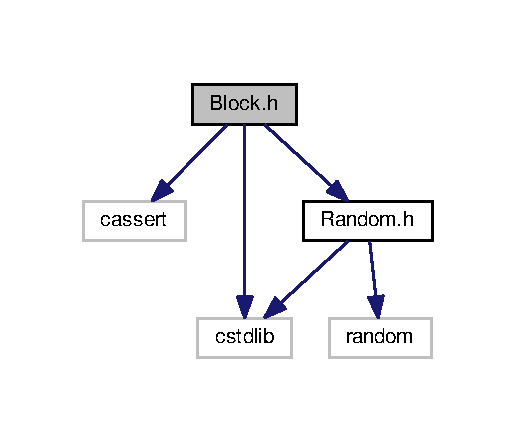
\includegraphics[width=320pt]{Block_8h__incl}
\end{center}
\end{figure}
This graph shows which files directly or indirectly include this file\+:
\nopagebreak
\begin{figure}[H]
\begin{center}
\leavevmode
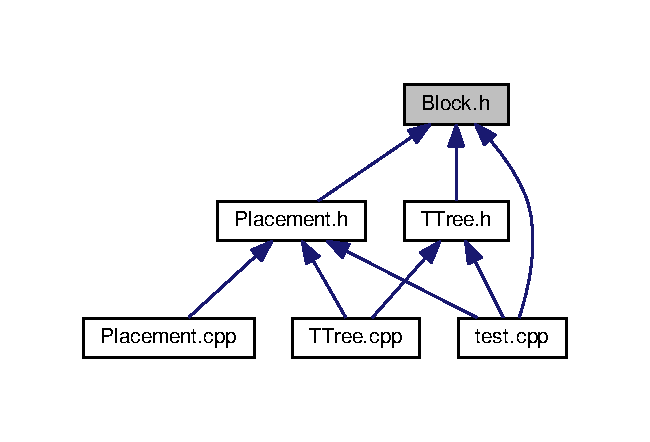
\includegraphics[width=350pt]{Block_8h__dep__incl}
\end{center}
\end{figure}
\subsection*{Classes}
\begin{DoxyCompactItemize}
\item 
struct \hyperlink{structBlock}{Block}
\begin{DoxyCompactList}\small\item\em Defines a block out of the coordinates. \end{DoxyCompactList}\item 
struct \hyperlink{structRotatableBlock}{Rotatable\+Block}
\end{DoxyCompactItemize}

\hypertarget{ContourList_8cpp}{}\section{Contour\+List.\+cpp File Reference}
\label{ContourList_8cpp}\index{Contour\+List.\+cpp@{Contour\+List.\+cpp}}
{\ttfamily \#include $<$cmath$>$}\\*
{\ttfamily \#include $<$cassert$>$}\\*
{\ttfamily \#include $<$algorithm$>$}\\*
{\ttfamily \#include \char`\"{}Contour\+List.\+h\char`\"{}}\\*
Include dependency graph for Contour\+List.\+cpp\+:
\nopagebreak
\begin{figure}[H]
\begin{center}
\leavevmode
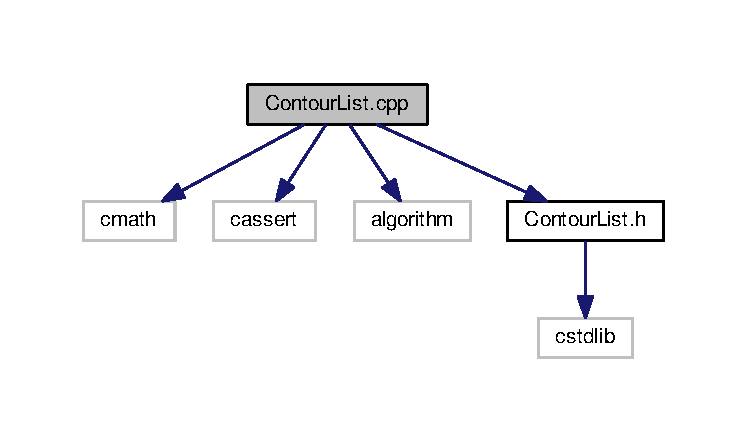
\includegraphics[width=350pt]{ContourList_8cpp__incl}
\end{center}
\end{figure}

\hypertarget{ContourList_8h}{}\section{Contour\+List.\+h File Reference}
\label{ContourList_8h}\index{Contour\+List.\+h@{Contour\+List.\+h}}
{\ttfamily \#include $<$cstdlib$>$}\\*
Include dependency graph for Contour\+List.\+h\+:
\nopagebreak
\begin{figure}[H]
\begin{center}
\leavevmode
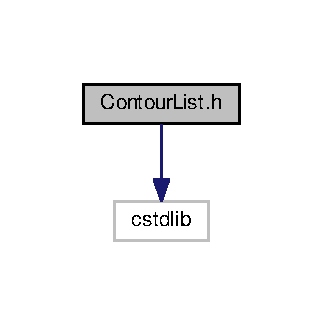
\includegraphics[width=155pt]{ContourList_8h__incl}
\end{center}
\end{figure}
This graph shows which files directly or indirectly include this file\+:
\nopagebreak
\begin{figure}[H]
\begin{center}
\leavevmode
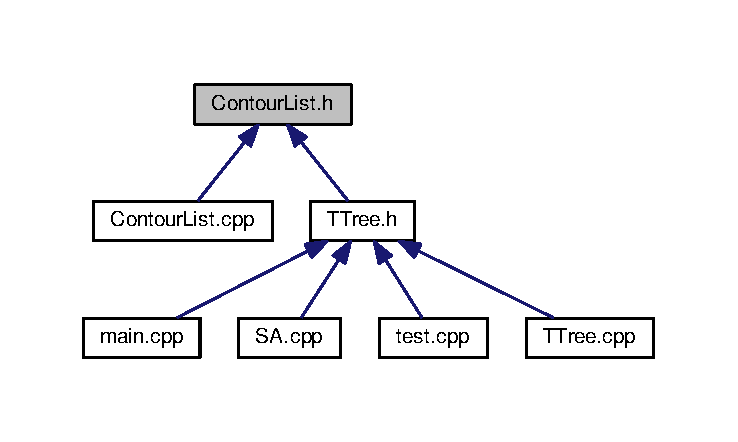
\includegraphics[width=277pt]{ContourList_8h__dep__incl}
\end{center}
\end{figure}
\subsection*{Classes}
\begin{DoxyCompactItemize}
\item 
class \hyperlink{classContourList}{Contour\+List}
\begin{DoxyCompactList}\small\item\em Defines a vertical contour doubly-\/linked list. used by \hyperlink{classTTree}{T\+Tree}. static class. \end{DoxyCompactList}\item 
struct \hyperlink{structContourList_1_1Node}{Contour\+List\+::\+Node}
\begin{DoxyCompactList}\small\item\em A node of a contour list. \end{DoxyCompactList}\end{DoxyCompactItemize}

\hypertarget{gen_8cpp}{}\section{gen.\+cpp File Reference}
\label{gen_8cpp}\index{gen.\+cpp@{gen.\+cpp}}
{\ttfamily \#include $<$ctime$>$}\\*
{\ttfamily \#include $<$cstdlib$>$}\\*
{\ttfamily \#include $<$iostream$>$}\\*
Include dependency graph for gen.\+cpp\+:
\nopagebreak
\begin{figure}[H]
\begin{center}
\leavevmode
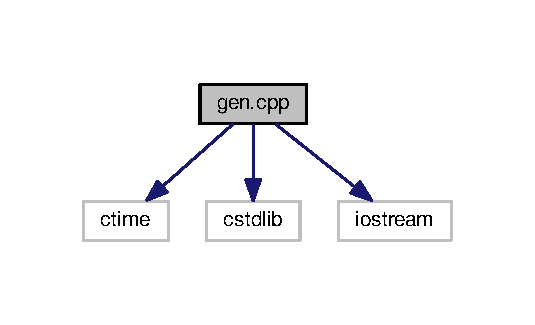
\includegraphics[width=257pt]{gen_8cpp__incl}
\end{center}
\end{figure}
\subsection*{Functions}
\begin{DoxyCompactItemize}
\item 
double \hyperlink{gen_8cpp_a60bca9fc56d141b9ec796c29b1abf0cc}{rand\+Double} (double l, double r)
\begin{DoxyCompactList}\small\item\em This program randomly generates the input It generates n blocks, where n is from the command line argument. \end{DoxyCompactList}\item 
int \hyperlink{gen_8cpp_a3c04138a5bfe5d72780bb7e82a18e627}{main} (int argc, char $\ast$$\ast$argv)
\end{DoxyCompactItemize}


\subsection{Function Documentation}
\hypertarget{gen_8cpp_a3c04138a5bfe5d72780bb7e82a18e627}{}\index{gen.\+cpp@{gen.\+cpp}!main@{main}}
\index{main@{main}!gen.\+cpp@{gen.\+cpp}}
\subsubsection[{main}]{\setlength{\rightskip}{0pt plus 5cm}int main (
\begin{DoxyParamCaption}
\item[{int}]{argc, }
\item[{char $\ast$$\ast$}]{argv}
\end{DoxyParamCaption}
)}\label{gen_8cpp_a3c04138a5bfe5d72780bb7e82a18e627}
\hypertarget{gen_8cpp_a60bca9fc56d141b9ec796c29b1abf0cc}{}\index{gen.\+cpp@{gen.\+cpp}!rand\+Double@{rand\+Double}}
\index{rand\+Double@{rand\+Double}!gen.\+cpp@{gen.\+cpp}}
\subsubsection[{rand\+Double}]{\setlength{\rightskip}{0pt plus 5cm}double rand\+Double (
\begin{DoxyParamCaption}
\item[{double}]{l, }
\item[{double}]{r}
\end{DoxyParamCaption}
)\hspace{0.3cm}{\ttfamily [inline]}}\label{gen_8cpp_a60bca9fc56d141b9ec796c29b1abf0cc}


This program randomly generates the input It generates n blocks, where n is from the command line argument. 

It outputs to stdout with the format below\+: The first line contains one number \+: n Each of the following line contains 3 numbers for each block as \+: x y hgen random double in range \mbox{[}l, r\mbox{]} 
\hypertarget{main_8cpp}{}\section{main.\+cpp File Reference}
\label{main_8cpp}\index{main.\+cpp@{main.\+cpp}}
{\ttfamily \#include $<$ctime$>$}\\*
{\ttfamily \#include $<$cmath$>$}\\*
{\ttfamily \#include $<$vector$>$}\\*
{\ttfamily \#include $<$string$>$}\\*
{\ttfamily \#include $<$fstream$>$}\\*
{\ttfamily \#include $<$sstream$>$}\\*
{\ttfamily \#include $<$iostream$>$}\\*
{\ttfamily \#include \char`\"{}S\+A.\+h\char`\"{}}\\*
{\ttfamily \#include \char`\"{}T\+Tree.\+h\char`\"{}}\\*
{\ttfamily \#include \char`\"{}Block.\+h\char`\"{}}\\*
{\ttfamily \#include \char`\"{}Placement.\+h\char`\"{}}\\*
Include dependency graph for main.\+cpp\+:
\nopagebreak
\begin{figure}[H]
\begin{center}
\leavevmode
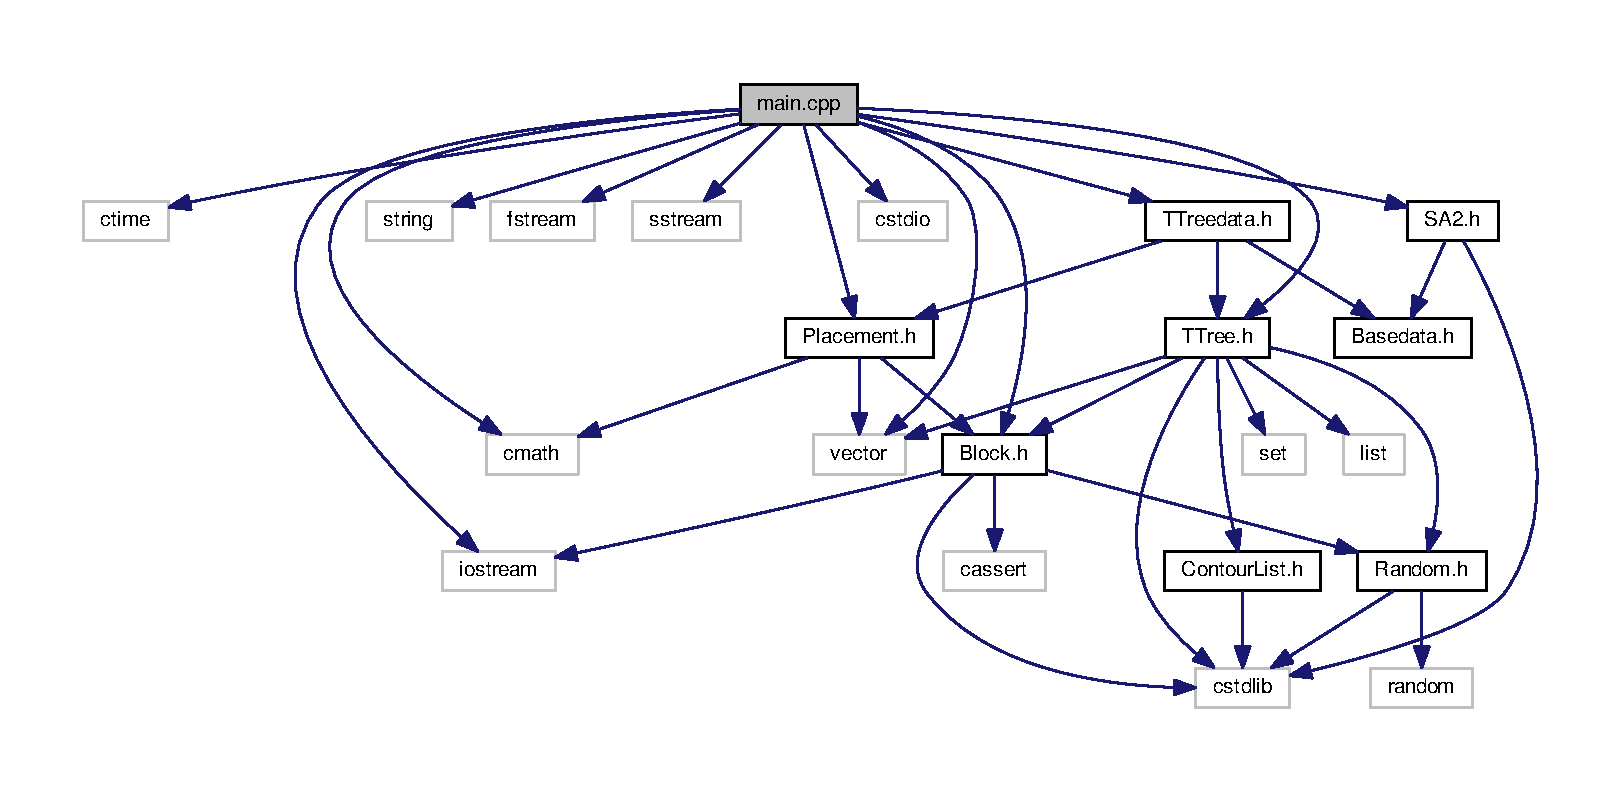
\includegraphics[width=350pt]{main_8cpp__incl}
\end{center}
\end{figure}
\subsection*{Functions}
\begin{DoxyCompactItemize}
\item 
void \hyperlink{main_8cpp_a897c0a0b24c1fa9b288631d3e1b1e469}{callback} (int step, double temperature, double accept\+Wasted\+Rate, double min\+Wasted\+Rate)
\begin{DoxyCompactList}\small\item\em Report every several steps. \end{DoxyCompactList}\item 
std\+::vector$<$ \hyperlink{structBlock}{Block} $>$ \hyperlink{main_8cpp_a19d3891e843c71c76daaddfa2563ed05}{load\+Blocks} (std\+::istream \&is)
\item 
\hyperlink{classSA}{S\+A} \hyperlink{main_8cpp_a3fa93a88f4ab7cdfa23dd68ce5c127b1}{load\+S\+A} (std\+::istream \&is, \hyperlink{classTTree}{T\+Tree} $\ast$tree)
\item 
int \hyperlink{main_8cpp_a3c04138a5bfe5d72780bb7e82a18e627}{main} (int argc, char $\ast$$\ast$argv)
\end{DoxyCompactItemize}


\subsection{Function Documentation}
\hypertarget{main_8cpp_a897c0a0b24c1fa9b288631d3e1b1e469}{}\index{main.\+cpp@{main.\+cpp}!callback@{callback}}
\index{callback@{callback}!main.\+cpp@{main.\+cpp}}
\subsubsection[{callback}]{\setlength{\rightskip}{0pt plus 5cm}void callback (
\begin{DoxyParamCaption}
\item[{int}]{step, }
\item[{double}]{temperature, }
\item[{double}]{accept\+Wasted\+Rate, }
\item[{double}]{min\+Wasted\+Rate}
\end{DoxyParamCaption}
)}\label{main_8cpp_a897c0a0b24c1fa9b288631d3e1b1e469}


Report every several steps. 

\hypertarget{main_8cpp_a19d3891e843c71c76daaddfa2563ed05}{}\index{main.\+cpp@{main.\+cpp}!load\+Blocks@{load\+Blocks}}
\index{load\+Blocks@{load\+Blocks}!main.\+cpp@{main.\+cpp}}
\subsubsection[{load\+Blocks}]{\setlength{\rightskip}{0pt plus 5cm}std\+::vector$<${\bf Block}$>$ load\+Blocks (
\begin{DoxyParamCaption}
\item[{std\+::istream \&}]{is}
\end{DoxyParamCaption}
)}\label{main_8cpp_a19d3891e843c71c76daaddfa2563ed05}
\hypertarget{main_8cpp_a3fa93a88f4ab7cdfa23dd68ce5c127b1}{}\index{main.\+cpp@{main.\+cpp}!load\+S\+A@{load\+S\+A}}
\index{load\+S\+A@{load\+S\+A}!main.\+cpp@{main.\+cpp}}
\subsubsection[{load\+S\+A}]{\setlength{\rightskip}{0pt plus 5cm}{\bf S\+A} load\+S\+A (
\begin{DoxyParamCaption}
\item[{std\+::istream \&}]{is, }
\item[{{\bf T\+Tree} $\ast$}]{tree}
\end{DoxyParamCaption}
)}\label{main_8cpp_a3fa93a88f4ab7cdfa23dd68ce5c127b1}
\hypertarget{main_8cpp_a3c04138a5bfe5d72780bb7e82a18e627}{}\index{main.\+cpp@{main.\+cpp}!main@{main}}
\index{main@{main}!main.\+cpp@{main.\+cpp}}
\subsubsection[{main}]{\setlength{\rightskip}{0pt plus 5cm}int main (
\begin{DoxyParamCaption}
\item[{int}]{argc, }
\item[{char $\ast$$\ast$}]{argv}
\end{DoxyParamCaption}
)}\label{main_8cpp_a3c04138a5bfe5d72780bb7e82a18e627}

\hypertarget{Placement_8cpp}{}\section{Placement.\+cpp File Reference}
\label{Placement_8cpp}\index{Placement.\+cpp@{Placement.\+cpp}}
{\ttfamily \#include $<$algorithm$>$}\\*
{\ttfamily \#include \char`\"{}Placement.\+h\char`\"{}}\\*
Include dependency graph for Placement.\+cpp\+:\nopagebreak
\begin{figure}[H]
\begin{center}
\leavevmode
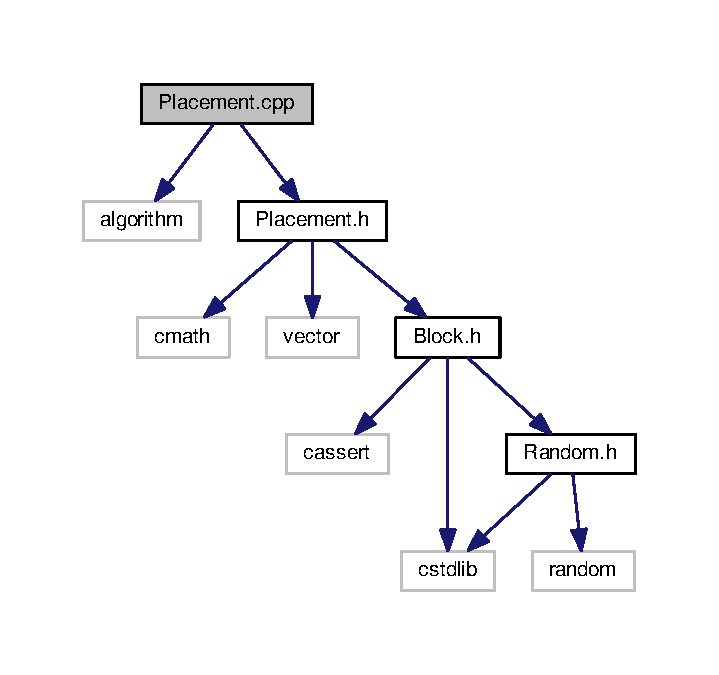
\includegraphics[width=345pt]{Placement_8cpp__incl}
\end{center}
\end{figure}

\hypertarget{Placement_8h}{}\section{Placement.\+h File Reference}
\label{Placement_8h}\index{Placement.\+h@{Placement.\+h}}
{\ttfamily \#include $<$cmath$>$}\\*
{\ttfamily \#include $<$vector$>$}\\*
{\ttfamily \#include \char`\"{}Block.\+h\char`\"{}}\\*
Include dependency graph for Placement.\+h\+:
\nopagebreak
\begin{figure}[H]
\begin{center}
\leavevmode
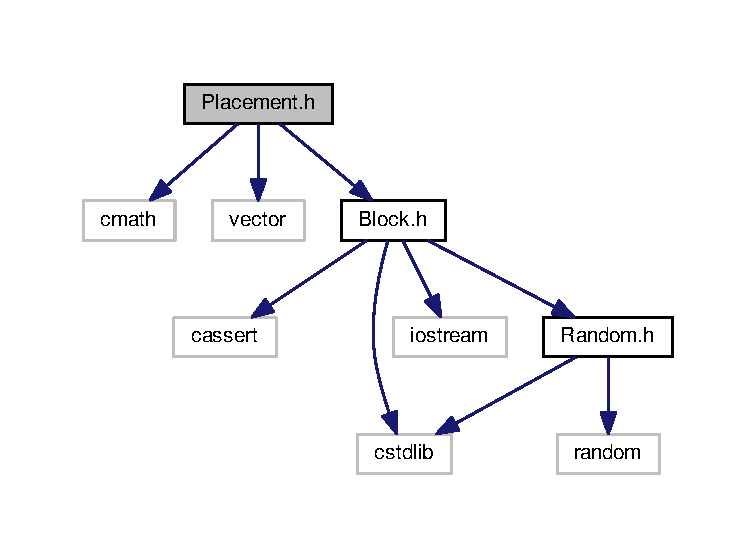
\includegraphics[width=319pt]{Placement_8h__incl}
\end{center}
\end{figure}
This graph shows which files directly or indirectly include this file\+:
\nopagebreak
\begin{figure}[H]
\begin{center}
\leavevmode
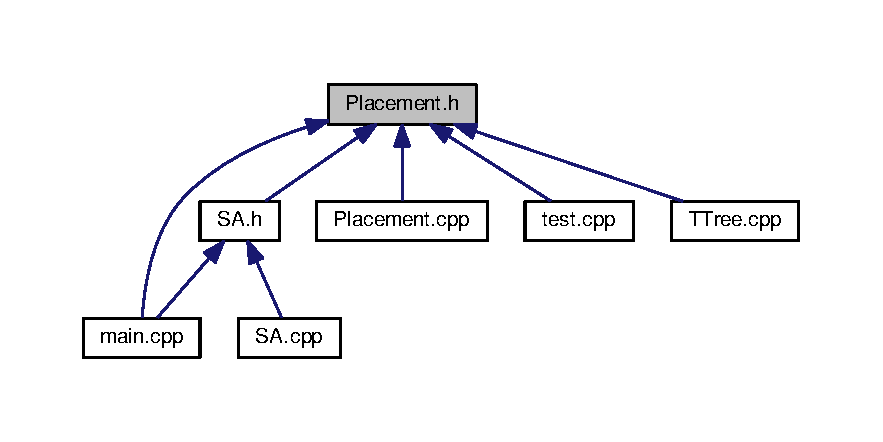
\includegraphics[width=312pt]{Placement_8h__dep__incl}
\end{center}
\end{figure}
\subsection*{Classes}
\begin{DoxyCompactItemize}
\item 
class \hyperlink{classPlacement}{Placement}
\begin{DoxyCompactList}\small\item\em A compact placement of blocks. \end{DoxyCompactList}\item 
struct \hyperlink{structPlacement_1_1BlockWithPos}{Placement\+::\+Block\+With\+Pos}
\end{DoxyCompactItemize}

\hypertarget{Random_8cpp}{}\section{Random.\+cpp File Reference}
\label{Random_8cpp}\index{Random.\+cpp@{Random.\+cpp}}
{\ttfamily \#include $<$ctime$>$}\\*
{\ttfamily \#include \char`\"{}Random.\+h\char`\"{}}\\*
Include dependency graph for Random.\+cpp\+:
\nopagebreak
\begin{figure}[H]
\begin{center}
\leavevmode
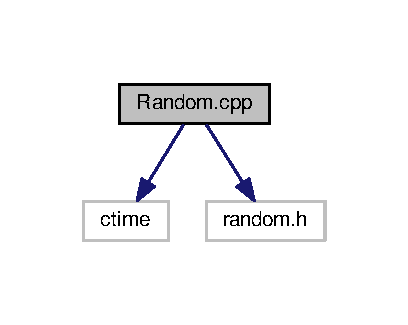
\includegraphics[width=227pt]{Random_8cpp__incl}
\end{center}
\end{figure}
\subsection*{Macros}
\begin{DoxyCompactItemize}
\item 
\#define \hyperlink{Random_8cpp_ad350bae49f72ba58d73027f1316e38b8}{S\+E\+E\+D}~0
\end{DoxyCompactItemize}


\subsection{Macro Definition Documentation}
\hypertarget{Random_8cpp_ad350bae49f72ba58d73027f1316e38b8}{}\index{Random.\+cpp@{Random.\+cpp}!S\+E\+E\+D@{S\+E\+E\+D}}
\index{S\+E\+E\+D@{S\+E\+E\+D}!Random.\+cpp@{Random.\+cpp}}
\subsubsection[{S\+E\+E\+D}]{\setlength{\rightskip}{0pt plus 5cm}\#define S\+E\+E\+D~0}\label{Random_8cpp_ad350bae49f72ba58d73027f1316e38b8}

\hypertarget{Random_8h}{}\section{Random.\+h File Reference}
\label{Random_8h}\index{Random.\+h@{Random.\+h}}
{\ttfamily \#include $<$cstdlib$>$}\\*
{\ttfamily \#include $<$random$>$}\\*
Include dependency graph for Random.\+h\+:\nopagebreak
\begin{figure}[H]
\begin{center}
\leavevmode
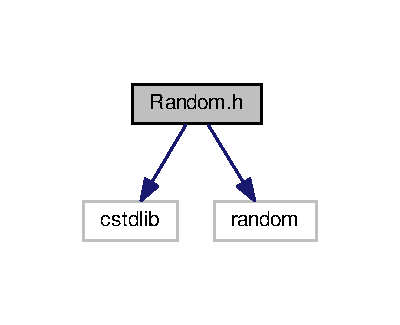
\includegraphics[width=192pt]{Random_8h__incl}
\end{center}
\end{figure}
This graph shows which files directly or indirectly include this file\+:\nopagebreak
\begin{figure}[H]
\begin{center}
\leavevmode
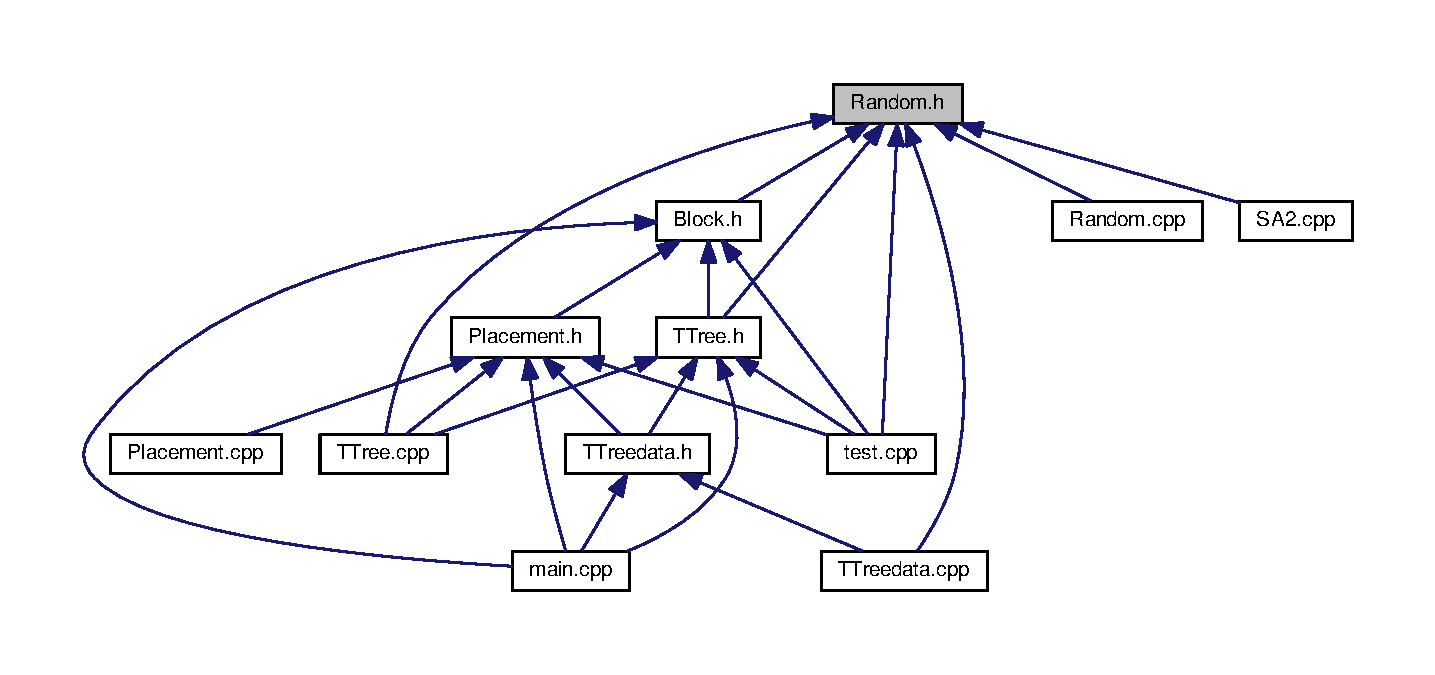
\includegraphics[width=312pt]{Random_8h__dep__incl}
\end{center}
\end{figure}
\subsection*{Classes}
\begin{DoxyCompactItemize}
\item 
class \hyperlink{classRandom}{Random}
\begin{DoxyCompactList}\small\item\em Please to this file instead of generate random numbers by yourself. It provide a consistent control of the seed. \end{DoxyCompactList}\end{DoxyCompactItemize}

\hypertarget{README_8md}{}\section{R\+E\+A\+D\+M\+E.\+md File Reference}
\label{README_8md}\index{R\+E\+A\+D\+M\+E.\+md@{R\+E\+A\+D\+M\+E.\+md}}

\hypertarget{SA2_8cpp}{}\section{S\+A2.\+cpp File Reference}
\label{SA2_8cpp}\index{S\+A2.\+cpp@{S\+A2.\+cpp}}
{\ttfamily \#include $<$cmath$>$}\\*
{\ttfamily \#include $<$cassert$>$}\\*
{\ttfamily \#include $<$iostream$>$}\\*
{\ttfamily \#include $<$cstdio$>$}\\*
{\ttfamily \#include \char`\"{}S\+A2.\+h\char`\"{}}\\*
{\ttfamily \#include \char`\"{}Random.\+h\char`\"{}}\\*
Include dependency graph for S\+A2.\+cpp\+:
\nopagebreak
\begin{figure}[H]
\begin{center}
\leavevmode
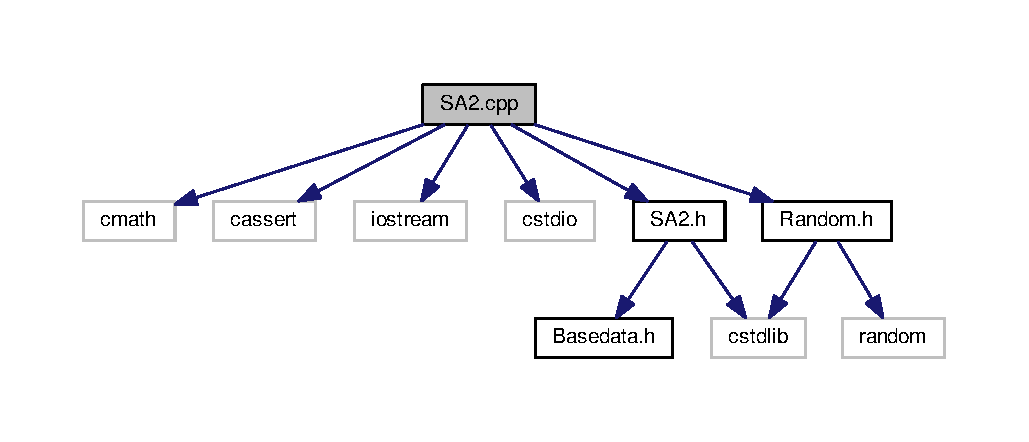
\includegraphics[width=350pt]{SA2_8cpp__incl}
\end{center}
\end{figure}

\hypertarget{SA2_8h}{}\section{S\+A2.\+h File Reference}
\label{SA2_8h}\index{S\+A2.\+h@{S\+A2.\+h}}
{\ttfamily \#include $<$cstdlib$>$}\\*
{\ttfamily \#include \char`\"{}Basedata.\+h\char`\"{}}\\*
Include dependency graph for S\+A2.\+h\+:
\nopagebreak
\begin{figure}[H]
\begin{center}
\leavevmode
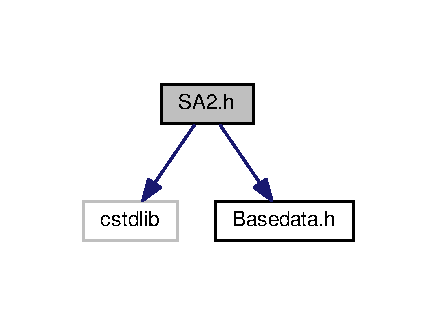
\includegraphics[width=210pt]{SA2_8h__incl}
\end{center}
\end{figure}
This graph shows which files directly or indirectly include this file\+:
\nopagebreak
\begin{figure}[H]
\begin{center}
\leavevmode
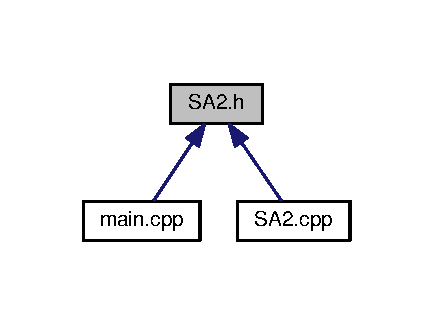
\includegraphics[width=208pt]{SA2_8h__dep__incl}
\end{center}
\end{figure}
\subsection*{Classes}
\begin{DoxyCompactItemize}
\item 
class \hyperlink{classSA__2}{S\+A\+\_\+2}
\begin{DoxyCompactList}\small\item\em Simulated Annealing. \end{DoxyCompactList}\end{DoxyCompactItemize}

\hypertarget{test_8cpp}{}\section{test.\+cpp File Reference}
\label{test_8cpp}\index{test.\+cpp@{test.\+cpp}}
{\ttfamily \#include $<$cassert$>$}\\*
{\ttfamily \#include $<$iostream$>$}\\*
{\ttfamily \#include \char`\"{}Block.\+h\char`\"{}}\\*
{\ttfamily \#include \char`\"{}T\+Tree.\+h\char`\"{}}\\*
{\ttfamily \#include \char`\"{}Random.\+h\char`\"{}}\\*
{\ttfamily \#include \char`\"{}Placement.\+h\char`\"{}}\\*
Include dependency graph for test.\+cpp\+:
\nopagebreak
\begin{figure}[H]
\begin{center}
\leavevmode
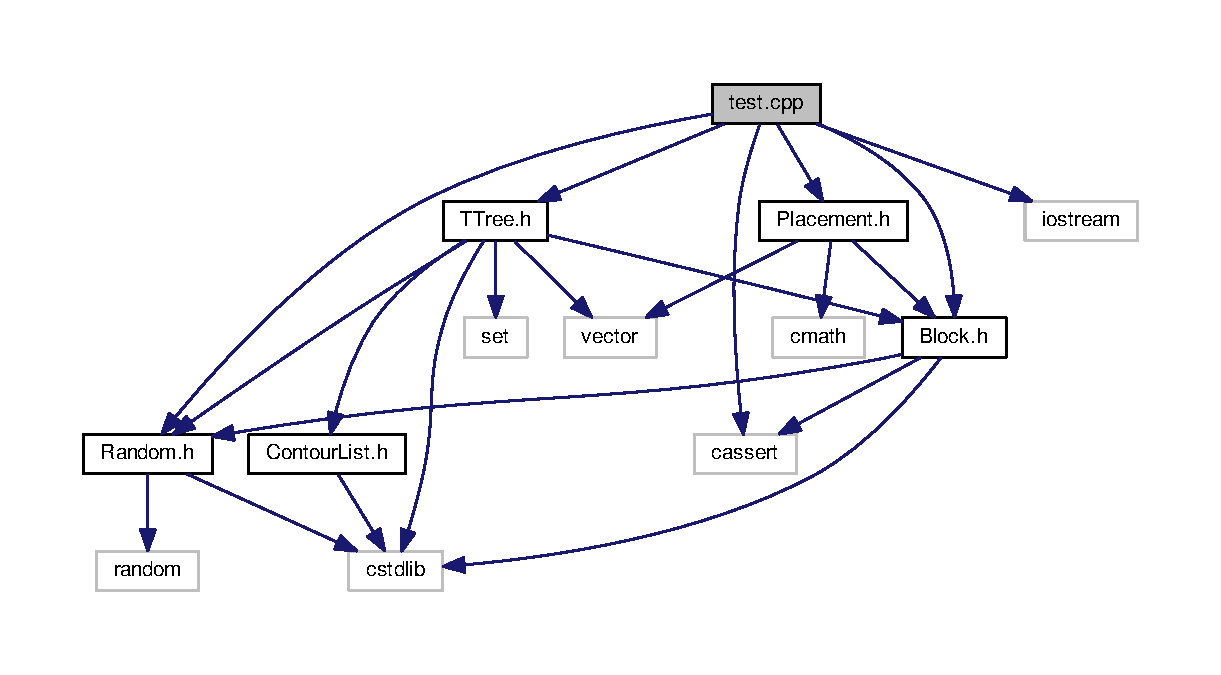
\includegraphics[width=350pt]{test_8cpp__incl}
\end{center}
\end{figure}
\subsection*{Functions}
\begin{DoxyCompactItemize}
\item 
int \hyperlink{test_8cpp_ae66f6b31b5ad750f1fe042a706a4e3d4}{main} ()
\end{DoxyCompactItemize}
\subsection*{Variables}
\begin{DoxyCompactItemize}
\item 
const int \hyperlink{test_8cpp_a39add79319612ddcf2cb59b2ed809ced}{block\+Num} = 500
\begin{DoxyCompactList}\small\item\em Compile with this file but without \hyperlink{main_8cpp}{main.\+cpp} to perform a test. \end{DoxyCompactList}\item 
const int \hyperlink{test_8cpp_aba7b88e0401b2719b8bd6e356d1c33dd}{test\+Num} = 100
\item 
const int \hyperlink{test_8cpp_af0d3619b7e5c98e05e6940cd5b1a760c}{perturb\+Num} = 100
\item 
const double \hyperlink{test_8cpp_a6405e942744ed21d4678c62f912ca748}{max\+Block\+Size} = 10
\end{DoxyCompactItemize}


\subsection{Function Documentation}
\hypertarget{test_8cpp_ae66f6b31b5ad750f1fe042a706a4e3d4}{}\index{test.\+cpp@{test.\+cpp}!main@{main}}
\index{main@{main}!test.\+cpp@{test.\+cpp}}
\subsubsection[{main}]{\setlength{\rightskip}{0pt plus 5cm}int main (
\begin{DoxyParamCaption}
{}
\end{DoxyParamCaption}
)}\label{test_8cpp_ae66f6b31b5ad750f1fe042a706a4e3d4}


\subsection{Variable Documentation}
\hypertarget{test_8cpp_a39add79319612ddcf2cb59b2ed809ced}{}\index{test.\+cpp@{test.\+cpp}!block\+Num@{block\+Num}}
\index{block\+Num@{block\+Num}!test.\+cpp@{test.\+cpp}}
\subsubsection[{block\+Num}]{\setlength{\rightskip}{0pt plus 5cm}const int block\+Num = 500}\label{test_8cpp_a39add79319612ddcf2cb59b2ed809ced}


Compile with this file but without \hyperlink{main_8cpp}{main.\+cpp} to perform a test. 

\hypertarget{test_8cpp_a6405e942744ed21d4678c62f912ca748}{}\index{test.\+cpp@{test.\+cpp}!max\+Block\+Size@{max\+Block\+Size}}
\index{max\+Block\+Size@{max\+Block\+Size}!test.\+cpp@{test.\+cpp}}
\subsubsection[{max\+Block\+Size}]{\setlength{\rightskip}{0pt plus 5cm}const double max\+Block\+Size = 10}\label{test_8cpp_a6405e942744ed21d4678c62f912ca748}
\hypertarget{test_8cpp_af0d3619b7e5c98e05e6940cd5b1a760c}{}\index{test.\+cpp@{test.\+cpp}!perturb\+Num@{perturb\+Num}}
\index{perturb\+Num@{perturb\+Num}!test.\+cpp@{test.\+cpp}}
\subsubsection[{perturb\+Num}]{\setlength{\rightskip}{0pt plus 5cm}const int perturb\+Num = 100}\label{test_8cpp_af0d3619b7e5c98e05e6940cd5b1a760c}
\hypertarget{test_8cpp_aba7b88e0401b2719b8bd6e356d1c33dd}{}\index{test.\+cpp@{test.\+cpp}!test\+Num@{test\+Num}}
\index{test\+Num@{test\+Num}!test.\+cpp@{test.\+cpp}}
\subsubsection[{test\+Num}]{\setlength{\rightskip}{0pt plus 5cm}const int test\+Num = 100}\label{test_8cpp_aba7b88e0401b2719b8bd6e356d1c33dd}

\hypertarget{TTree_8cpp}{}\section{T\+Tree.\+cpp File Reference}
\label{TTree_8cpp}\index{T\+Tree.\+cpp@{T\+Tree.\+cpp}}
{\ttfamily \#include $<$cmath$>$}\\*
{\ttfamily \#include $<$cassert$>$}\\*
{\ttfamily \#include $<$algorithm$>$}\\*
{\ttfamily \#include \char`\"{}T\+Tree.\+h\char`\"{}}\\*
{\ttfamily \#include \char`\"{}Random.\+h\char`\"{}}\\*
{\ttfamily \#include \char`\"{}Placement.\+h\char`\"{}}\\*
Include dependency graph for T\+Tree.\+cpp\+:\nopagebreak
\begin{figure}[H]
\begin{center}
\leavevmode
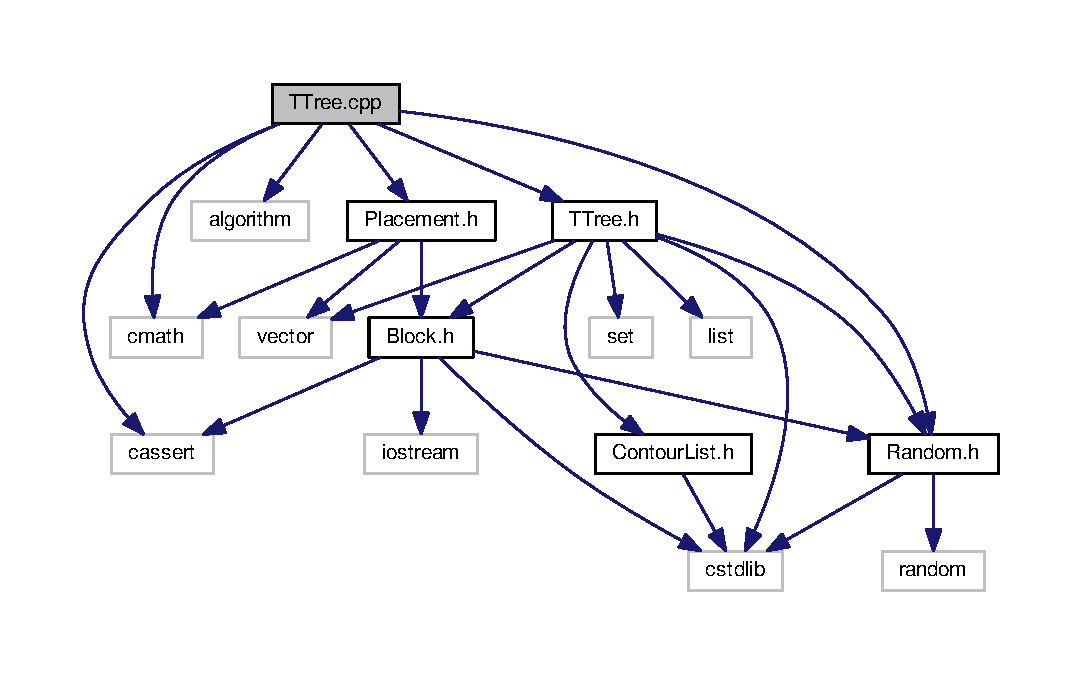
\includegraphics[width=350pt]{TTree_8cpp__incl}
\end{center}
\end{figure}

\hypertarget{TTree_8h}{}\section{T\+Tree.\+h File Reference}
\label{TTree_8h}\index{T\+Tree.\+h@{T\+Tree.\+h}}
{\ttfamily \#include $<$cstdlib$>$}\\*
{\ttfamily \#include $<$set$>$}\\*
{\ttfamily \#include $<$vector$>$}\\*
{\ttfamily \#include \char`\"{}Block.\+h\char`\"{}}\\*
{\ttfamily \#include \char`\"{}Random.\+h\char`\"{}}\\*
{\ttfamily \#include \char`\"{}Contour\+List.\+h\char`\"{}}\\*
Include dependency graph for T\+Tree.\+h\+:\nopagebreak
\begin{figure}[H]
\begin{center}
\leavevmode
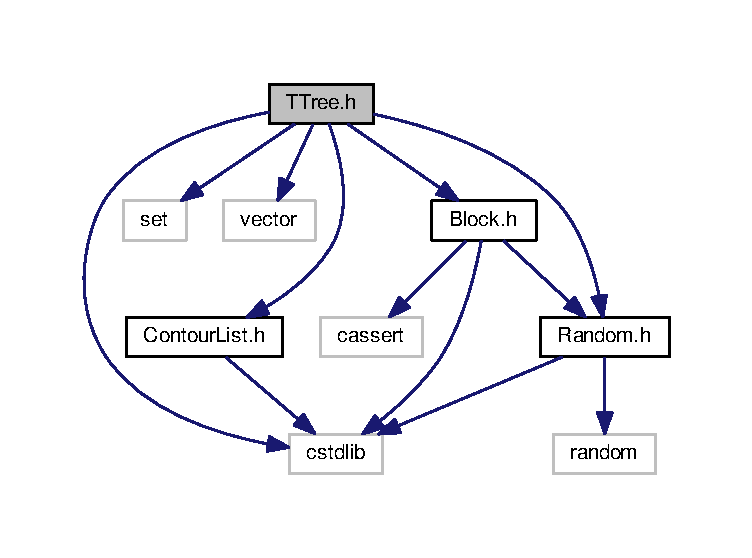
\includegraphics[width=350pt]{TTree_8h__incl}
\end{center}
\end{figure}
This graph shows which files directly or indirectly include this file\+:\nopagebreak
\begin{figure}[H]
\begin{center}
\leavevmode
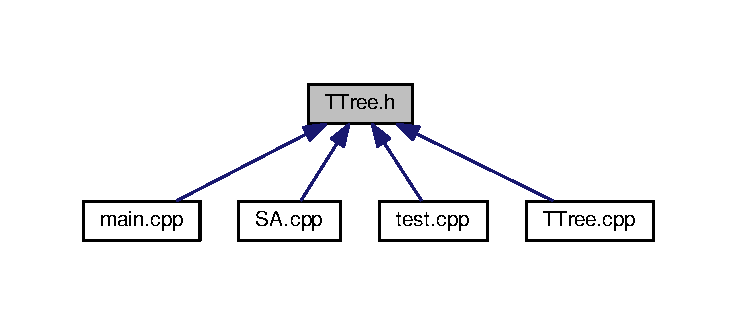
\includegraphics[width=212pt]{TTree_8h__dep__incl}
\end{center}
\end{figure}
\subsection*{Classes}
\begin{DoxyCompactItemize}
\item 
class \hyperlink{classTTree}{T\+Tree}
\item 
struct \hyperlink{structTTree_1_1Node}{T\+Tree\+::\+Node}
\begin{DoxyCompactList}\small\item\em Internal class. A node of T Tree. \end{DoxyCompactList}\end{DoxyCompactItemize}

\hypertarget{TTreedata_8cpp}{}\section{T\+Treedata.\+cpp File Reference}
\label{TTreedata_8cpp}\index{T\+Treedata.\+cpp@{T\+Treedata.\+cpp}}
{\ttfamily \#include \char`\"{}T\+Treedata.\+h\char`\"{}}\\*
{\ttfamily \#include \char`\"{}Random.\+h\char`\"{}}\\*
Include dependency graph for T\+Treedata.\+cpp\+:
\nopagebreak
\begin{figure}[H]
\begin{center}
\leavevmode
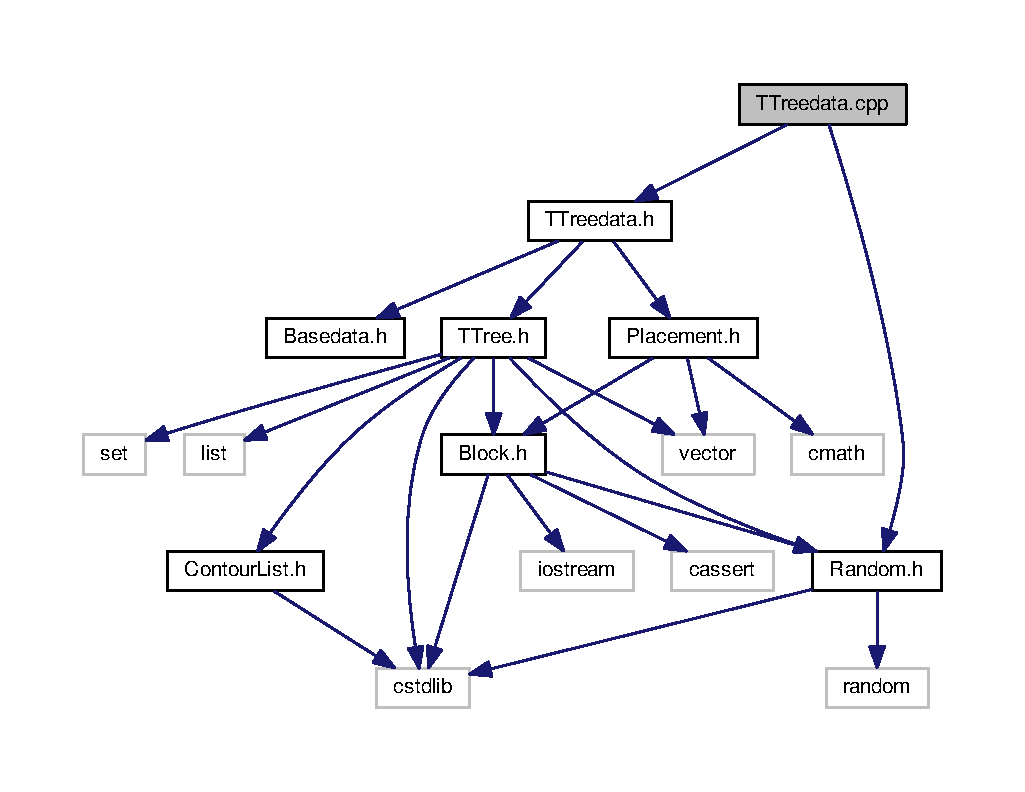
\includegraphics[width=350pt]{TTreedata_8cpp__incl}
\end{center}
\end{figure}

\hypertarget{TTreedata_8h}{}\section{T\+Treedata.\+h File Reference}
\label{TTreedata_8h}\index{T\+Treedata.\+h@{T\+Treedata.\+h}}
{\ttfamily \#include \char`\"{}Basedata.\+h\char`\"{}}\\*
{\ttfamily \#include \char`\"{}T\+Tree.\+h\char`\"{}}\\*
{\ttfamily \#include \char`\"{}Placement.\+h\char`\"{}}\\*
Include dependency graph for T\+Treedata.\+h\+:
\nopagebreak
\begin{figure}[H]
\begin{center}
\leavevmode
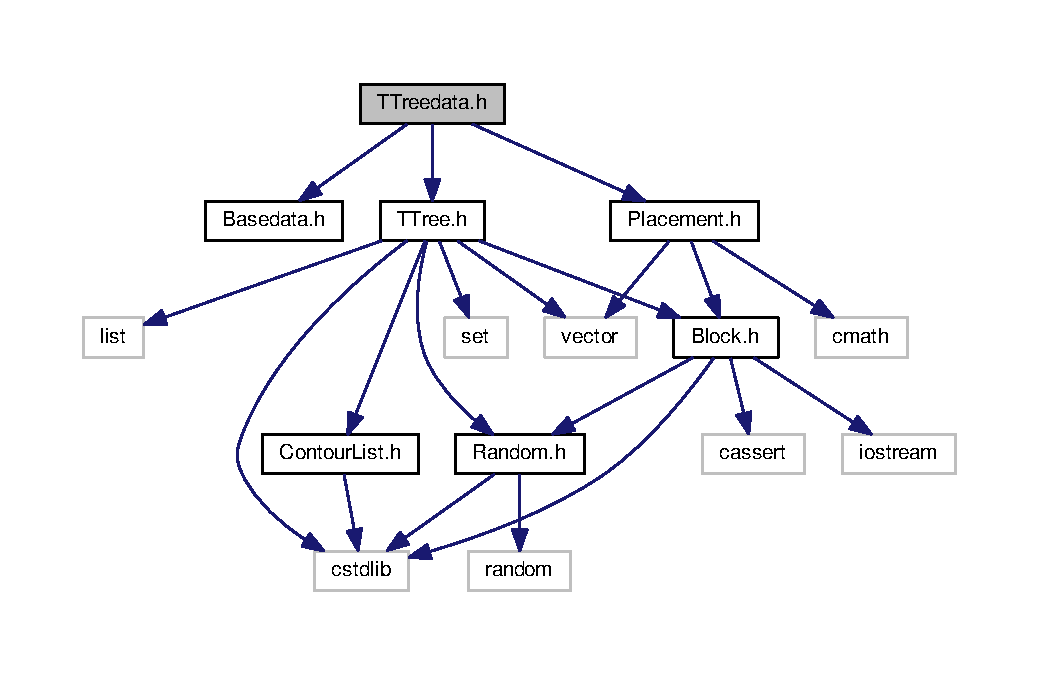
\includegraphics[width=350pt]{TTreedata_8h__incl}
\end{center}
\end{figure}
This graph shows which files directly or indirectly include this file\+:
\nopagebreak
\begin{figure}[H]
\begin{center}
\leavevmode
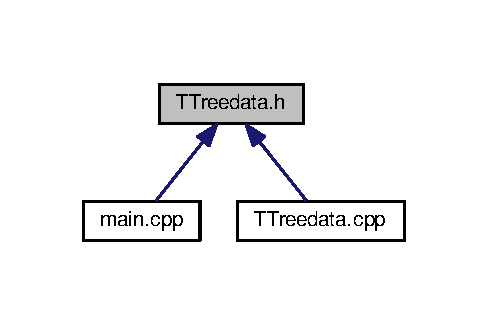
\includegraphics[width=234pt]{TTreedata_8h__dep__incl}
\end{center}
\end{figure}
\subsection*{Classes}
\begin{DoxyCompactItemize}
\item 
class \hyperlink{classTTree__data}{T\+Tree\+\_\+data}
\end{DoxyCompactItemize}

%--- End generated contents ---

% Index
\backmatter
\newpage
\phantomsection
\clearemptydoublepage
\addcontentsline{toc}{chapter}{Index}
\printindex

\end{document}
